\documentclass[10pt,openright,twoside,a4paper]{book}
%\linespread{1.1}

%Packages
\usepackage[vcentering,dvips]{geometry}                 % for making it 170 x 240 mm
\geometry{papersize={170mm,240mm},total={130mm,185mm}}  % I changed 195 to 185 because I have subscript areas The area of text of Marco is 130 x 195mm
\addtolength{\evensidemargin}{-0.85cm} \addtolength{\oddsidemargin}{0.85cm}% slightly unbalance the left and right pages
\usepackage{graphicx}		% include graphics
\usepackage{dcolumn}
\usepackage{bm}
\usepackage[toc,page,title,titletoc]{appendix}
\usepackage[caption=false]{subfig}
\usepackage{fancyhdr}		% fancy header and footer
\usepackage[T1]{fontenc}
\usepackage{ae,aecompl}             % computer modern in T1 encoding.
\usepackage{amssymb,amsmath}
\usepackage{afterpage}
\usepackage[normal,small,bf,up]{caption}
\usepackage{wrapfig}
%\usepackage[normal,footnotesize,bf,up]{caption}
%\usepackage[english]{babel}
\usepackage[active]{srcltx}  %SRC Specials for DVI search
\usepackage{url} %clickable urls
%\selectlanguage{english}
\newenvironment{abstract}{\rightskip1in\itshape}{}	%to allow abstract in every chapter
\renewcommand{\thefootnote}{\fnsymbol{footnote}}
\hfuzz2pt % Don't bother to report over-full boxes if over-edge is < 2pt
\pagestyle{headings}

%\usepackage{epsfig}
%\usepackage{hyperref}	% make a pdf with links
%\usepackage{float}
%\usepackage{sectsty}                % for customizing section headings.
%\usepackage{textcomp}               % for the trademark symbol.
%\usepackage{varioref}               % nice references.
%\usepackage{placeins}
%\usepackage{booktabs}
%\usepackage[square,sort&compress,numbers]{natbib}

%-------------------------------------
%% BIBLIOGRAPHY:
\usepackage[sectionbib]{chapterbib} %bib in every chapter
%\usepackage[sectionbib]{natbib}%does this work to get a sorted reference list?
%\citestyle{nature}
\renewcommand{\bibname}{References} %  will print "REFERENCES" instead of "BIBLIOGRAPHY"

% to have the chapter title in the center with an horizontal line on the name...
\makeatletter %from http://zoonek.free.fr/LaTeX/LaTeX_samples_chapter/0.html
\def\thickhrulefill{\leavevmode \leaders \hrule height 1ex \hfill \kern \z@}
\def\@makechapterhead#1{%
  \vspace*{10\p@}%
  {\parindent \z@ \centering \reset@font
        {\Huge\bfseries \thechapter }
        \par\nobreak
        \vspace*{10\p@}%
        \interlinepenalty\@M
        \hrule
        \vspace*{10\p@}%
        \Huge \bfseries #1\par\nobreak
        \par
        \vspace*{10\p@}%
    \vskip 100\p@
  }}
\def\@makeschapterhead#1{%
  \vspace*{10\p@}%
  {\parindent \z@ \centering \reset@font
        {\Huge\bfseries \vphantom{\thechapter} }
        \par\nobreak
        \vspace*{10\p@}%
        \interlinepenalty\@M
        \hrule
        \vspace*{10\p@}%
        \Huge \bfseries #1\par\nobreak
        \par
        \vspace*{10\p@}%
    \vskip 100\p@
  }}

%%% Fancy Header %%%%%%%%%%%%%%%%%%%%%%%%%%%%%%%%%%%%%%%%%%%%%%%%%%%%%%%%%%%%%%%%%%
% Fancy Header Style Options
\pagestyle{fancy}                       % Sets fancy header and footer
\fancyhf{} % clear all header and footer fields

% left page footer
%\fancyfoot[LE,RO]{\sffamily\footnotesize UltraCold Ion Beam Source}

% right page footer
%\fancyfoot[C]{\sffamily\footnotesize -- Confidential --}
\fancyfoot[CO]{\sffamily\footnotesize Nicola Debernardi}
\fancyfoot[CE]{\sffamily\footnotesize Eindhoven University of Technology}

\renewcommand{\chaptermark}[1]{\markboth{\chaptername\ \thechapter.\ #1}{}} % Lower Case Chapter marker style
\renewcommand{\sectionmark}[1]{\markright{\thesection.\ #1}}         % Lower case Section marker style
\fancyhead[LE,RO]{\bfseries\thepage}    % Page number (boldface) in left on even
                                        % pages and right on odd pages
\fancyhead[RE]{\bfseries\leftmark}      % Chapter in the right on even pages
\fancyhead[LO]{\bfseries\rightmark}     % Section in the left on odd pages
\renewcommand{\headrulewidth}{0.3pt}    % Width of head rule
\renewcommand{\footrulewidth}{0.3pt}    % Width of foot rule
%\renewcommand{\footskip}{3pt}              % Distance of foot rule from text body

%%% Clear Header %%%%%%%%%%%%%%%%%%%%%%%%%%%%%%%%%%%%%%%%%%%%%%%%%%%%%%%%%%%%%%%%%%
% Clear Header Style on the Last Empty Odd pages
\makeatletter
\def\cleardoublepage{\clearpage\if@twoside \ifodd\c@page\else%
    \hbox{}%
    \thispagestyle{empty}%              % Empty header styles
    \newpage%
    \if@twocolumn\hbox{}\newpage\fi\fi\fi}
\makeatother

\makeatletter \DeclareRobustCommand\onlinecite{\@onlinecite}
\def\@onlinecite#1{\begingroup\let\@cite\NAT@citenum\citealp{#1}\endgroup}
\makeatother
%%%%%%%%%%%%%%%%%%%%%%%%%%%%%%%%%%%%%%%%%%%%%%%%%%%%%%%%%%%%%%%%%%%%%%%%%%%%%%%%%%%%

\begin{document}

\pagenumbering{Roman}

\date{\today}
\frontmatter
\thispagestyle{empty} \vspace*{10mm}
\begin{center}
\Huge{\bfseries UltraCold}\\
\Huge{\bfseries Ion Beam}\\
\Huge{\bfseries Source}\\[2cm]


\LARGE PROEFSCHRIFT\\[2cm]\fontsize{14}{14}\selectfont
ter verkrijging van de graad van doctor aan de

Technische Universiteit Eindhoven, op gezag van de

rector magnificus, prof.dr.ir. C.J. van Duijn, voor een

commissie aangewezen door het College voor

Promoties in het openbaar te verdedigen

op woensdag 9 mei 2012 om 16.00 uur\\[1.5cm]
door\\[1.5cm]
Nicola Debernardi\\[1.5cm]
geboren te Biella, Itali\"{e}

\end{center}
\newpage
\thispagestyle{empty} \vspace*{-3mm}
\vspace*{-34pt}\fontsize{10}{50}
%\selectfont\noindent
\normalsize\noindent
Dit proefschrift is goedgekeurd door de promotor:\\%[-14mm]

%\normalsize
\noindent
prof.dr.ir. O.J. Luiten\\[0.5cm]

\noindent Copromotoren:\\
dr.ir. P.H.A. Mutsaers\\
en\\
dr.ir. E.J.D. Vredenbregt\\[5.5cm]

\noindent
Printed by Universiteitsdrukkerij Technische Universiteit Eindhoven.\\[10mm]
Cover designed by N. Debernardi (www.dobermaniprod.biz) using parts of figure \ref{fig:focusing_img}. Note that the contrast has been increased with respect to the original and the spiral has simply a graphical purpose, to better illustrate the focusing effect. \\%[10mm]
\hspace*{1mm}\\

\noindent
A catalogue record is available from the Eindhoven University of Technology Library\\
ISBN: 978-90-386-3138-7\\
NUR 926\\

\noindent
The work described in this thesis has been carried out at the group Coherence and Quantum Technology at the Eindhoven University of Technology, Department of Applied Physics, Den Dolech 2, 5612 AZ Eindhoven, the Netherlands.

\begin{figure}[h]
\includegraphics[height=1.0cm]{pics/stw.eps}   %[height=0.15\textwidth]
\end{figure}
\vspace*{-0.5cm}\noindent
This research is supported by the Dutch Technology Foundation STW, which is part of the Netherlands Organisation for Scientific Research (NWO) and partly funded by the Ministry of Economic Affairs, Agriculture and Innovation (ETF 07728).\\

\noindent Copyright \copyright~2012, N. Debernardi

\newpage

  
%if you want to dedicate the thesis to someone:
\newpage
\pagestyle{empty} \mbox{} \vfill
\begin{flushright}
\sl
\Large{Alla mia famiglia}\\
\Large{e ai miei amici.}\\
\end{flushright}
\cleardoublepage

\pagestyle{fancy}
\markboth{Contents}{} % toegevoegd in een poging de capitals te onderdrukken
  \setcounter{page}{1}
  \tableofcontents

\vspace{5 cm}
This thesis is partially based on the following publications:
\begin{itemize}
  \item Chapter \ref{ch:tempmea}:\\
  \underline{N. Debernardi}, M.P. Reijnders, W.J. Engelen, T.T.J. Clevis, P.H.A. Mutsaers, O.J. Luiten, and E.J.D. Vredenbregt, \textit{Measurement of the temperature of an ultracold ion source using time-dependent electric fields}, published in J. Appl. Phys. \textbf{110}, 024501 (2011).
 \item Chapter \ref{ch:currentmea}:\\
  \underline{N. Debernardi}, R.W.L. van Vliembergen, W.J. Engelen, K.H.M. Hermans, M.P. Reijnders, S.B. van der Geer, P.H.A. Mutsaers, O.J. Luiten, and E.J.D. Vredenbregt, \textit{Optimization of the current extracted from an ultracold ion source}, submitted to New J. Phys.
 \item Chapter \ref{ch:newsource}:\\
  \underline{N. Debernardi}, R.P.M.J.W. Notermans, D.J.N. Kusters, S.B. van der Geer, P.H.A. Mutsaers, O.J. Luiten and E.J.D. Vredenbregt, \textit{High brightness ion beam through magneto-optical compression}, submitted to New J. Phys.
\end{itemize}

\mainmatter
  \pagenumbering{arabic}
 \documentclass[12pt]{iopart}
%\documentclass[12pt,a4paper]{paper}

\usepackage{graphicx}% Include figure files
\usepackage{dcolumn}% Align table columns on decimal point1
\usepackage{bm}% bold math
\usepackage[caption=false]{subfig}

\begin{document}
\title{Introduction}

%\chapter[Introduction]{Introduction\label{ch:intro}}

\begin{abstract}
The work in this thesis covers the research on two kinds of laser-cooled ion sources for focused ion beam (FIB) applications. An ion source is an apparatus capable of providing ions preferably with a high current density. This section summarizes the applications of FIBs and gives an overview over the existing ion sources. The reduced brightness and the emittance are useful figures of merit used to characterize an ion source and a definition is here given. Those definitions are used through the chapters to compare the performances of the sources. Finally, an outline of this thesis is given at the end of this chapter.
\end{abstract}

\section{Overview over focused ion beam applications}
Miniaturization is a central theme in modern fabrication technology and many of the components used in modern products are becoming smaller and smaller \cite{Moore_E_65}. Nanotechnology tools have to keep up with this trend by improving minimum achievable resolution. FIB systems have in common high-brightness ion sources capable of producing high current density beams \cite{Orloff_RoSI_93, Orloff_Book_03}. Those machines can create structures with few nanometer precision, remove or add material through ion bombardment or beam-induced chemistry. Imaging is also possible, although damages are dominant at the smallest scales. Figure \ref{fig:applications}, shows three examples of the most common applications of FIBs. 
\begin{figure}[tbh!]
    \centering
    \subfloat[Imaging]{
        \label{a1}
        \includegraphics[width=0.3\linewidth]{appl1}}
    \hspace{.1in}
    \subfloat[Milling]{
        \label{a2}
        \includegraphics[width=0.3\linewidth]{appl2}}
    \hspace{.1in}
    \subfloat[Deposition]{
        \label{a3}
        \includegraphics[width=0.3\linewidth]{appl3}}
    \caption{Three examples of application of FIBs. The figure is taken from \cite{Reyntjens2001}.}
    \label{fig:applications}
\end{figure}

A focused ion beam microscope operates along the same principle as the scanning electron microscope (SEM), in that a beam of charged particles is scanned across a specimen, and the resultant signals at each raster position are plotted to form an image. The signal comes from a multichannel plate detector (MCP), see figure \ref{a1}. However, in FIBs the charged particle beam consists not of electrons, but rather of ions, which are typically positively charged. Because of the short De Broglie wavelength of the ions, FIBs have achieved spatial resolution rivaling that of the standard scanning electron microscope. Today's state-of-the-art FIBs are capable of imaging with a few nm spatial resolution, using secondary electrons or ions, i.e. secondary ion mass spectrometry (SIMS). Figure \ref{fig:FIBschem} shows a typical schematic of a FIB ion column.
\begin{figure}[tbh!]
    \centering
        \includegraphics[width=0.5\linewidth]{FIBschem}
    \caption{Schematic drawing of a FIB column \cite{Reyntjens2001}.}
    \label{fig:FIBschem}
\end{figure}
The ion are produced by the source on the top of the column. After a first refinement through the spray aperture, the ion beam is condensed in the first electrostatic lens and the spherical aberration is reduced with an octopole. The variable aperture is used to skim the beam to the desirable current. Blanking of the beam is accomplished by the blanking
deflector and aperture, while the lower octopole is used for raster scanning the beam over the sample in a user-defined pattern. In the second electrostatic lens, the beam is focused to a fine spot. The multichannel plate (MCP) is used to detect secondary particles for imaging.

The use of FIBs as precision sectioning tools down to sub-micron scale, creating a precise cut or cross-section from a few tens of nm with positional placement accuracy on the order of 20~nm is well exploited in the industry, see figure \ref{a2}. FIB has recently become a popular tool in making high-quality microdevices or high-precision microstructures \cite{Tseng2004}. Also, their ability to deposit metals and insulators on a micron scale is of large importance, introducing several different gases into the vacuum chamber to either deposit a range of materials up to tens of micrometers thickness over areas ranging from the sub-micrometers to tens of thousands of square micrometers or selectively etch one material rapidly, see figure \ref{a3}. 

Moreover, FIB have been adopted into the product cycle of semiconductor manufacturers in the late 1980s. In 1986, the number of FIB fabrication systems totaled about 35; in 1998, the number has increased 15-25 times \cite{Phaneuf1999}. FIBs are highly exploited in device modification, mask repair, process control and failure analysis \cite{Glanville1989, Ward1988, Stewart1995}. 
Even more, the preparation of specimens for transmission electron microscopy (TEM) is an important application \cite{Walker1995}.


\section{Overview of the existing ion sources for FIBs}
In the past few years, the interest on focused ion beams has seen another significant increase also because of the development of few distinct ion sources, which can expand the capabilities of these instruments. FIB system based on high-brightness \cite{Hagen_J_08} gallium liquid-metal ion sources (LMIS) became commercially available in the late 1980s. The LMIS \cite{Orloff_Book_03} is still currently the most used source in commercial instruments. The current is extracted from an extremely sharp tip (of the diameter of several nanometers) by applying high electric fields. Gallium is the most used element in the LMIS and this is also an important limitation for these sources. Expanding the choice of atomic species beyond gallium opens up FIBs to new applications on the market. Also, the resolution of LMIS is chromatic aberration limited to a few nanometers due to the energy spread of the source. The resolution of the LMIS will not be enough in the near future. The gas field ionization source (GFIS) \cite{Ward_JVSTB_06} replaces the heavy Ga$^+$ ions with much lighter He$^+$ (Ne$^+$) ions, enabling a very high resolution imaging. Long lifetime (this only applies to the Helium source, for Neon the lifetime is up to ten hours \cite{Notte2010}) and high brightness operation are its most important features. The resolution obtained with an ion microscope based on GFIS is probably unbeatable, but the milling capacities are quite poor. Especially due to the high penetration in the sample, the sputter yield is very low, almost neglecting the advantage of having a really high brightness \cite{Tan2010}. In order to improve the milling application, an inductive-coupled plasma source is being developed \cite{Smith2006}. This source uses Ar$^+$ and Xe$^+$ ion beams that can remove material almost contamination-free.

Laser-cooled ion sources as the ultracold ion source (UCIS) \cite{Claessens2005} and the magneto-optical trap ion source (MOTIS) \cite{Hanssen_PRA_06}, promises to expand the choice of ions available for FIB applications and aim to improve the milling and circuit editing capability for FIBs. Those sources can in principle be configured to produce ions of over twenty different elements \cite{Steele_JVSTB_10}. Both of the sources use the principle of laser-cooling and trapping of neutral atoms \cite{Metcalf_Book_99}, which are photo-ionized and accelerated to form a ion beam or ion bunches. Those sources aim to achieve high brightness, comparable to the one of the LMIS, by a very low transversal temperature (a few hundreds of microkelvin) of the ions, rather than extracting the ions from a ``point source''. Having an extended source is advantageous for the energy spread because space charge density is reduced and the probe is less sensitive to vibrations and instabilities, as one typically experiences with point sources. Because of these characteristic of the source, sub-micrometer focus-ability has been demonstrated \cite{Steele_JVSTB_10}. The energy spread has been measured down to 20 meV \cite{Reijnders_PRL_09}. Time-dependent manipulation of ion bunches has been shown in references \cite{Reijnders_PRL_10, Reijnders_JAP_11} and is successfully used for the measurement presented in chapter 3.

%To avoid disorder-induced heating of the UCIS \cite{Geer_JAP_07} and the MOTIS \cite{Steele_JAP_11}, another laser-cooled source with a much higher particle flux is proposed in chapter 6. 

Finally, laser-cooled sources have been successful in the production of bright electron beams for ultrafast electron diffraction \cite{Taban_EPL_10, Mcculloch2011}. 

\section{Source characterization: useful figures of merit}
When characterizing an ion source, only two figures of merit are of most importance: the brightness and the longitudinal energy spread.

%The reduced (transversal) brightness $B_r$ \cite{Luiten2007} is the current density per unit of solid angle and beam energy and is a in Lorentz-invariant. In units of [A/m$^2$~sr~eV], the reduced brightness is defined as
%\begin{equation}
%	B_r = \frac{2 I}{4 \pi^2 m c^2 \epsilon_n^x \epsilon_n^y},
%	\label{eq:red_brightness_intro}
%\end{equation}
%where $I$ is the current and $\epsilon_n^x$ and $\epsilon_n^y$ are the normalized \textit{rms}-emittance of the beam in the $x$ and $y$ direction (in this thesis, the ions always propagate along the $z$-axis). In the previous equation, a factor $e$ (the elementary charge) is removed in order to express the unit of brightness in $eV$ instead of $V$. The normalized \textit{rms}-emittance $\epsilon_n^x$ is defined as
%\begin{equation}
%	\epsilon_n^x = \frac{1}{m c} \sqrt{\langle x^2 \rangle \langle p_x^2 \rangle - \langle x p_x \rangle^2} = \frac{1}{c} \sqrt{\langle x^2 \rangle \langle v_x^2 \rangle - \langle x v_x \rangle^2}.
%	\label{eq:norm_emittance_intro}
%\end{equation}
%where $c$ is the speed of light, $x$ is the position of a particle and the notation $\langle~\rangle$ implies an average over a set of particles. In the previous equation, the substitution of the non-relativistic momentum $p_x = m v_x$ is used (ions at energies up to 15~keV are non-relativistic). The normalized \textit{rms} emittance $\epsilon_y^n$ is defined similarly. Filling equation (\ref{eq:norm_emittance_intro}) in equation (\ref{eq:red_brightness_intro}), the reduced brightness can be rewritten as
The reduced (transversal) brightness $B_r$ \cite{Luiten2007} is the current density per unit of solid angle. In units of [A/m$^2$~sr~eV] is given by
\begin{equation}
	B_r = \frac{I}{4 \pi^2 \epsilon_r^x \epsilon_r^y},
	\label{eq:red_brightness2_intro}
\end{equation}
where the reduced emittance in the $x$-direction $\epsilon_r^x$ is
\begin{equation}
	\epsilon_r^x = \sqrt{\frac{m}{2}} \sqrt{\langle x^2 \rangle \langle v_x^2 \rangle - \langle x v_x \rangle^2}.
	\label{eq:red_emittance_intro}
\end{equation}
Equation (\ref{eq:red_emittance_intro}) can be derived from the usual definition of reduced emittance $\epsilon_r^x=\sigma_x \sigma_{x'} \sqrt{U}$ that can be found in literature. A similar equation holds for the quantity $\epsilon_r^y$. In this thesis, the ions always propagate along the $z$-axis.\\

The \textit{rms} energy spread $\sigma_U$ of an UCIS is an intrinsic property of the source. It is proportional to the accelerating field $E_0$ and the ionization laser \textit{rms} radius $\sigma_i$ as
\begin{equation}
	\sigma_U = e E_0 \sigma_i.
	\label{eq:en_spread}
\end{equation}

The attainable spot size $d$ in a FIB \cite{Kruit1997}, for a chromatic aberration limited source, is connected to the energy spread and the brightness as
\begin{equation}
	d=\left(\frac{I~C_C^2~\sigma_U^2}{B_r~V_p^3}\right)^{1/4},
	\label{eq:minspot}
\end{equation}
where $C_C$ is the chromatic aberration coefficient of the focusing system, $I$ is the ion beam current and $V_p$ is the voltage applied to accelerate the ions. Typically, $C_C=20$~mm and $V_p=30$~kV for FIB columns \cite{Geer_JAP_07}.

%\begin{table}[tbh!]
% \caption{Summary of the characteristics of the ion sources for FIBs.}
%\begin{tabular}{}
%
%    \label{tab:sources}
%                                          & \textbf{UCIS}                       & \textbf{LMIS}                         & \textbf{FES} \\
%                                          & Ultra Cold                          & Liquid Metal                          & Field Emission        \\
%                                          & Ion Source                          &       Ion Source                      &   Source \\
%
%    \textbf{Properties}\\
%                \hspace{10mm}Current $I$  & $0-100\rm~pA$                       & $0-10\rm~nA$                          & $0-100\rm~pA$\\
%                \\
%                \hspace{10mm}Ion species  & Alkali metals                       & Ga                                    & He\\
%                                          & (e.g. Li, Cs), \\
%                                          & Alkaline earth metals,\\
%                                          & Cr, Yb, \\
%                                          & Nobel gasses, ...\\
%
%    \textbf{Beam quality (1 pA)}  \\
%    \hspace{10mm}Brightness $B_r$         & $3 \times 10^5$                     & $1 \times 10^6$                       & $5 \times 10^8$\\
%                                          & \small{A/(m$^{2}$ sr V)}            & \small{A/(m$^{2}$ sr V)}              & \small{A/(m$^{2}$ sr V)}\\
%    \\
%    \hspace{10mm}Energy spread $\Delta U$ & $0.2~\rm eV$                        & $4.5~\rm eV$ \cite{LMIS-energyspread}  & $<1.0~\rm eV$ \cite{He-microscope2}\\
%    \\
%    \hspace{10mm} Source radius $R$       & $4.5\rm~\mu m$                      & $25~\rm nm$ \cite{LMIS-brightness1}    & $\sim 0.3~\rm nm$ \cite{He-microscope2}\\
%    \hspace{10mm} (effective)\\
%    \\
%    \hspace{10mm}Temperature $T$          & $150\rm~\mu K$                      &                                       & \\
%
%\end{tabular}
%\end{table}


\section{This thesis}
This thesis is mainly made up as a collection of three scientific papers, already published or submitted for publication (chapters 3, 4 and 5). In chapter 2, the experimental setup is presented, focusing on some details that were not covered in the publications. Chapter 3 and 4 are based on experimental measurements of the UCIS. Chapter 3 deals with the measurement of the source temperature. An upper limit of the emittance is there obtained and this chapter introduces a new technique used to focus an ion beam with the use of time-dependent electric fields. In chapter 4, a model of the source is presented and validated with measurements. Then, the current of the UCIS is measured and finally simulations of disorder-induced heating are presented. The general conclusion is that the UCIS can not increase the brightness and at the same time decrease the longitudinal energy spread beyond that of the LMIS: one of the two quantities needs to be sacrificed with respect to the other one. To overcome this problem, chapter 5 presents a new kind of source, also based on laser-cooling, and summarize a series of simulations where it is shown that even with taking into account the disorder induced heating, the source performs better than the LMIS. Finally, chapter 6 summarizes the main conclusions of the thesis and gives an outlook for the future of laser-cooled ion sources for FIBs.\\

\bibliographystyle{unsrt}
%\bibliography{biblio}

\begin{thebibliography}{10}

\bibitem{Moore_E_65}
G.~E.~Moore.
\newblock {C}ramming more components onto integrated circuits.
\newblock {\em Electronics}, 38/8, 1965.

\bibitem{Orloff_RoSI_93}
J.~Orloff.
\newblock {H}igh-resolution focused ion beams.
\newblock {\em Rev. Sci. Instrum.}, 64(5):1105--1130, 1993.

\bibitem{Orloff_Book_03}
J.~Orloff, M.~Utlaut, and Swanson L.
\newblock {\em {H}igh {R}esolution {F}ocused {I}on {B}eams: {FIB} and {I}ts
  {A}pplications}.
\newblock Kluwer Academic, 2003.

\bibitem{Reyntjens2001}
S.~Reyntjens and R.~Puers.
\newblock A review of focused ion beam applications in microsystem technology.
\newblock {\em J. Micromech. Microeng.}, 11:287--300, 2001.

\bibitem{Phaneuf1999}
M.~W. Phaneuf.
\newblock Applications of focused ion beam mcroscopy to material scence
  specimens.
\newblock {\em Micron}, 30:277--288, 1999.

\bibitem{Glanville1989}
J.~Glanville.
\newblock Focused ion beam technology for integrated circuit modification.
\newblock {\em Solid State Technol.}, 32:270, 1989.

\bibitem{Ward1988}
B.~W. Ward, N.~P. Economou, D.~C. Shaver, J.~E. Ivory, M.~L. Ward, and L.~A.
  Stern.
\newblock Microcircuit modification using focused ion beams.
\newblock In {\em Proc. SPIE}, page~92, 1988.

\bibitem{Stewart1995}
D.~K. Stewart, A.~F. Doyle, and Casey J.~D. Jr.
\newblock Focused ion beam deposition of new materials: dielectric films for
  device modification and mask repair, and ta films for x-ray mask repair.
\newblock In {\em Proc. SPIE}, page 276, 1995.

\bibitem{Walker1995}
J.~F. Walker, J.~C. Reiner, and C.~Solenthaler.
\newblock Focused ion beam sample preparation for tem.
\newblock In {\em Proc. Microsc. Semicond. Mater. Conf.}, page 629, 1995.

\bibitem{Tseng2004}
A.~A. Tseng.
\newblock Recent developments on micromilling using focused ion beam
  technology.
\newblock {\em J. Micromech. Microeng}, 14:R15--R34, 2004.

\bibitem{Hagen_J_08}
C.~W. Hagen, E.~Fokkema, and P.~Kruit.
\newblock {B}rightness measurements of a gallium liquid metal ion source.
\newblock {\em J Vac Sci Technol B}, 26(6):2091--2096, 2008.

\bibitem{Ward_JVSTB_06}
B.W. Ward, J.A. Notte, and N.P. Economou.
\newblock {H}elium ion microscope: {A} new tool for nanoscale microscopy and
  metrology.
\newblock {\em J. Vac. Sci. Technol. B}, 24/6:2871--2874, 2006.

\bibitem{Tan2010}
S.Tan, R. Livengood, D. Shima, J. Notte, and S. McVey.
\newblock 54th international conference on electron, ion and photon beam technology and nanofabrication / Focused Ion Beams.
\newblock In {\em Gas field ion source and liquid metal ion source charged particle material interaction study for semiconductor nanomachining applications}. J. Vac. Sci. Technol. B 28, C6F15, 2010.

\bibitem{Notte2010}
J. Notte, F. Rahman, S. McVey, S. Tan, and R. H. Livengood
\newblock Neon Gas Field Ion Source � Stability and Lifetime.
\newblock {\em Microsc. and Microanal.}, 16(2), 2010.

\bibitem{Smith2006}
N.~S. Smith, W.~P. Skoczylas, S.~M. Kellogg, D.~E. Kinion, P.~P. Tesch,
  O.~Sutherland, A.~Aanesland, and R.~W. Boswell.
\newblock High brightness inductively coupled plasma source for high current
  focused ion beam applications.
\newblock {\em J. Vac. Sci. Technol. B}, 24(6):2902--2906, 2006.

\bibitem{Claessens2005}
B.~J. Claessens, S.~B. van~der Geer, G.~Taban, E.~J.~D. Vredenbregt, and O.~J.
  Luiten.
\newblock {U}ltracold {E}lectron {S}ource.
\newblock {\em Phys. Rev. Lett.}, 95(16):164801, 2005.

\bibitem{Hanssen_PRA_06}
J.~L. Hanssen, J.~J. McClelland, E.~A. Dakin, and M.~Jacka.
\newblock {L}aser-cooled atoms as a focused ion-beam source.
\newblock {\em Phys. Rev. A: At. Mol. Opt. Phys.}, 74(6):063416, 2006.

\bibitem{Steele_JVSTB_10}
A.~V. Steele, B.~Knuffman, J.~J. McClelland, and J.~Orloff.
\newblock {F}ocused chromium ion beam.
\newblock {\em J Vac Sci Technol B}, 28(6):C6F1--C6F5, 2010.

\bibitem{Metcalf_Book_99}
H.J. Metcalf and P.~van~der Straten.
\newblock {\em {L}aser {C}ooling and {T}rapping}.
\newblock Springer, 1999.

\bibitem{Reijnders_PRL_09}
M.~P. Reijnders, P.~A. van Kruisbergen, G.~Taban, S.~B. van~der Geer, P.~H.~A.
  Mutsaers, E.~J.~D. Vredenbregt, and O.~J. Luiten.
\newblock {L}ow-{E}nergy-{S}pread {I}on {B}unches from a {T}rapped {A}tomic
  {G}as.
\newblock {\em Phys. Rev. Lett.}, 102(3):034802, 2009.

\bibitem{Reijnders_PRL_10}
M.~P. Reijnders, N.~Debernardi, S.~B. van~der Geer, P.~H.~A. Mutsaers, E.~J.~D.
  Vredenbregt, and O.~J. Luiten.
\newblock {P}hase-{S}pace {M}anipulation of {U}ltracold {I}on {B}unches with
  {T}ime-{D}ependent {F}ields.
\newblock {\em Phys. Rev. Lett.}, 105(3):034802, 2010.

\bibitem{Reijnders_JAP_11}
M.~P Reijnders, N.~Debernardi, S.B. van~der Geer, P.H.A. Mutsaers, E.J.D.
  Vredenbregt, and O.J. Luiten.
\newblock {T}ime-dependent manipulation of ultracold ion bunches.
\newblock {\em J. Appl. Phys.}, 109:033302, 2011.

\bibitem{Geer_JAP_07}
S.~B. van~der Geer, M.~P. Reijnders, M.~J. de~Loos, E.~J.~D. Vredenbregt,
  P.~H.~A. Mutsaers, and O.~J. Luiten.
\newblock {S}imulated performance of an ultracold ion source.
\newblock {\em J. Appl. Phys.}, 102(9):094312, 2007.

\bibitem{Steele_JAP_11}
A.~V. Steele, B.~Knuffman, and J.~J. McClelland.
\newblock {I}nter-ion coulomb interactions in a magneto-optical trap ion
  source.
\newblock {\em J. Appl. Phys.}, 109(10):104308, 2011.

\bibitem{Taban_EPL_10}
G.~Taban, M.~P. Reijnders, B.~Fleskens, S.~B. van~der Geer, O.~J. Luiten, and
  E.~J.~D. Vredenbregt.
\newblock {U}ltracold electron source for single-shot diffraction studies.
\newblock {\em EPL (Europhysics Letters)}, 91(4):46004, 2010.

\bibitem{Mcculloch2011}
A.~J. Mcculloch, D.~V. Sheludko, M.~Junker, S.~C. Bell, S.~D. Saliba, K.~A.
  Nugent, and R.~E. Scholten.
\newblock Arbitrary shaped high-coherence electron bunches from ultracold
  plasma.
\newblock {\em Nature Physics}, 7:785--788, 2011.

\bibitem{Luiten2007}
O.~J. Luiten, B.~J. Claessens, S.~B. van~der Geer, M.~P. Reijnders, G.~Taban,
  and E.~J.~D. Vredenbregt.
\newblock Proceedings of the 46th workshop of the infn eloisatron project.
\newblock In {\em The physics and applications of high brightness electron
  beams}. World Scientific Publishing Co. Pte. Ltd., 2007.
  
\bibitem{Kruit1997}
P.~Kruit, and H.~Jansen.
\newblock {\em Space charge and statistical Coulomb effects}.
\newblock in {\em Handbook of charged particle optics}.
\newblock Ed. Jon Orloff, CRC Press, New York, 1997.
  
\end{thebibliography}

\end{document}
 \documentclass[12pt]{iopart}
%\documentclass[12pt]{article}

\usepackage{graphicx}% Include figure files
\usepackage{dcolumn}% Align table columns on decimal point1
\usepackage{bm}% bold math
\usepackage[caption=false]{subfig}

\begin{document}
\title{Experimental setup}

%\chapter[Experimental setup]{Experimental setup\label{ch:setup}}vdHeijden11\cite


\begin{abstract}
Chapters 3 and 4 already describe the experimental setup, not in much detail. This section is meant to cover what was left out in those two articles. The setup has been already extensively described in the PhD dissertations of Reijnders \cite{Reijnders2010} and Taban \cite{Taban2009}. The beam line and the MOT chamber are described in the first two sections. The laser setup is shown in section 3. Information about the calibration and the resolution of the MCP detector, playing an important role in the measurement of chapters 3 and 4, are given in section 4 and 5.
\end{abstract}


\section{Beam line}
The experimental setup is schematically drawn in figure \ref{fig:beamline}.
\begin{figure}[tbh!]
	\centering
		\includegraphics[width=1\linewidth]{beamline}
	\caption{Schematic drawing of the beam line used to measure the properties of the UCIS. The $y$-direction is pointing toward the reader. \label{fig:beamline}}
\end{figure}
The ions are created in the magneto-optical trap (MOT) chamber on the left hand side of the figure at $z=0$ and travel about 1.5~m in the beam line until the detector, shown on the right hand side. The MOT is located in a vacuum chamber, where the typical pressure is kept below $10^{-8}$~mbar by a pumping system (two ion gatter pumps), not shown in figure \ref{fig:beamline}.  The MOT chamber is discussed in section \ref{MOTchamber}. The first valve is meant to keep the MOT chamber independent from the beam line, in case that is not under vacuum. A pair of deflector plates are used to steer the beam in the $x$ and $y$-directions. An articulated feature, right after the deflectors, permits to move the beam line up to the the detector within an angle of about $5\,^{\circ}$. A retractable Faraday cup can be inserted in the beam line and with the use of an electrometer, it can measure the charge of ion bunches and eventually the current of an ion beam. The detector setup and the required calibration are discussed in section \ref{sec:calibrationMCP}. The detector is kept at a low pressure with an ion gatter pump, when the second valve is closed. The same ion pump is used to keep the pressure in the beam line at about $10^{-7}$~mbar, when the second valve is open. The turbo pump, connected with the beam line through the third valve, is used to pre-pump the beam line. During the experiment, the third valve third valve is kept closed and the turbo pump is not running. 


\section{Magneto optical trap chamber} \label{MOTchamber}
The UCIS setup uses a standard $^{85}$Rb magneto-optical trap configuration \cite{Metcalf_Book_99}. Atoms are cooled with three orthogonal pairs of counter propagating circularly polarized laser beams (trapping lasers) and are trapped by a quadrupole magnetic field. The magnetic field gradient of about 1~G/mm is generated by two coils placed in an anti-Helmholtz configuration. The trapping beams together with the magnetic field gradient slow down and trap the atoms in the center of the MOT. The MOT contains about $2 \times 10^8$ $^{85}$Rb$^+$ atoms in a \textit{rms}-radius of about 1~mm. 

The relevant hyperfine energy levels of $^{85}$Rb are plotted in figure \ref{fig:RbLevels}, where the used laser transitions are also presented. Details about the laser setup are given in section \ref{sec:lasers}.
\begin{figure}[tbh!]
	\centering
	\includegraphics[width=0.5\textwidth]{leveldiagram}
	\caption{The relevant hyperfine energy levels of $^{85}$Rb and the used laser transitions (see next section). The continuum marked by $\infty$ is the ionized state. The figure is edited from reference \cite{Claessens06}. \label{fig:RbLevels}}
\end{figure}
The atoms that are trapped in the MOT, are continuously excited by the trapping laser to the 5P$_{3/2}$,F=4 state, and then decay back to the 5S$_{1/2}$,F=3 ground state. However, since the hyperfine levels are not that far apart, some of the trapping laser power will actually excite the transition to the 5P$_{3/2}$,F=3 state. These atoms can than decay to the ``wrong'' ground state 5S$_{1/2}$,F=2. In order to make sure that these atoms do not get pumped to that state, a repump laser is needed. This pumps the atoms back to the 5P$_{3/2}$,F=3 state, from where they can also decay to the ``right'' ground state, 5S$_{1/2}$,F=3. The repump laser is left on all time. 

A schematic representation of the vacuum chamber can be found in figure \ref{fig:setup_MOT}.
\begin{figure}[tbh!]
	\centering
		\includegraphics[width=0.7\linewidth]{setup_MOT}
	\caption{Schematic overview of the vacuum chamber that contains the MOT and accelerator structure \cite{Taban2009}. One of the trapping laser beam pairs is shown, namely the horizontal beam pair. This pair consists of two separate laser beams, which are reflected by mirrors before they reach the MOT. It is not exactly horizontal, because in that case the mirror on the right would block the outcoming ion beam. The other pairs are diagonal beams in the $(x,y)$-plane, which are back-reflected. The coils that create the magnetic field gradient are also indicated in the figure. Finally, there are two cameras observing the fluorescence of the MOT, only the top one is shown. The side camera is behind the setup, looking toward the reader. \label{fig:setup_MOT}}
\end{figure}
The electric field strength at the starting point $z=0$ is 0.37 kV/cm per kV input voltage $V_a$ and $U = e V_a/2.05$, where $e$ is the elementary charge. The accelerator is rotationally symmetric and designed for voltages up to 30~kV. With a DC accelerating field, the exit of the accelerator forms an aperture lens with a negative focal length $f_0$ of 33 mm (``exit kick'' effect), which is independent of the acceleration voltage. For more details of the accelerator structure see \cite{Taban2009}. 

As the trapping lasers continuously excite the trapped atoms, they send out spontaneously emitted photons. Two CCD cameras observe the fluorescence of the MOT, one from the top and one from the side, continuously determining the density and the dimension of the MOT. The number of trapped atoms $N$ is given by
\begin{equation}
	N = \frac{P \lambda}{h \gamma f (\Omega / 4 \pi)},
\end{equation}
where $P$ is the power of the emitted light, $\lambda=780$~nm is the wavelength of the emitted light, $h$ is Planck's constant, $\gamma = 2 \pi \cdot 5.98$~MHz is the decay rate from the excited state, $f \approx 0.5$ is the fraction of excited atoms and finally $\Omega / 4 \pi$ is the solid angle seen by the camera. Details on the geometrical configuration and the calibration of the cameras can be found in \cite{Hermans10}. 


\section{Laser setup} \label{sec:lasers}
Lasers form an important part of the setup. They are needed first to cool down the atoms and also to ionize the cooled atoms. Four different lasers are used in the lab and their properties are summarized in table \ref{tab:lasers}.
\begin{table}[tbh!]
\caption{\label{tab:lasers} Lasers used in the experiments.}
\begin{center}
  \begin{tabular}{ | l | l | l | l | l | }
  \hline
  Laser 				& Used to           & Wavelength & Power / Energy  	& Pulse length					\\ \hline
  Toptica DLX 110 		& trap		& 780 nm 		& 900~mW		& CW		 					\\
  Toptica DL 100 		& repump 		& 780 nm 		& 100~mW 		& CW		  					\\
  Quanta-Ray PDL3 		& ionize		& 479.1 nm 		& 0.1~mJ			& 2.5~ns \textit{rms}	\\
  Toptica TA-SHG 110 	& ionize		& 479.1 nm 		& 250~mW 		& CW							\\ \hline
  \end{tabular}
\end{center}
\end{table}

The trapping and repump laser need to be stabilized to within a few megahertz. For the trapping laser beam, this is achieved with modulation transfer spectroscopy. The repump laser is locked with respect to the trapping laser, separated 3~GHz in frequency away. More details about the laser locking can be found in \cite{Reijnders2010}. 
The difference in frequency between the trapping laser and excitation laser is very small ($\Delta f=-14.5$~MHz), therefore a single laser is used for both transitions. Moreover,  the laser power needed for the excitation laser beam is only a small fraction of that needed for the trapping laser beams since the trapping laser beams are much larger than the excitation laser beam. The trapping laser beams carry 250~mW of laser power in total, while the excitation laser beam uses at most only 10~mW of it. The detuning and intensity of the excitation and trapping laser beams are controlled using acousto-optic modulators (AOMs) which in turn are computer controlled by a programmable pattern generator (PPG). The PPG has an internal clock that operates at 50~MHz, so its resolution is 20~ns. The PPG is used to synchronize and computer control most of the experimental setup.

The ionization transition is that of the excited atoms from any of the 5P$_{3/2}$ states to just above the ionization threshold. Note that atoms can only be ionized if they are first excited. For the experiment presented in this thesis (chapters 3 and 4), the CW ionization laser is used. The pulsed dye laser is used as an ionization laser only in the calibration of the MCP, see section \ref{sec:calibrationMCP}. The continuous ionization laser beam can be switched on and off with an acousto-optical deflector (AOD), which is also computer controlled.

The photo-ionization takes place in the small region of the atom cloud where both the excitation laser and ionization laser are present, the core region. This is schematically represented in figure \ref{fig:coreVolume}.
\begin{figure}[tbh!]
	\centering
		\includegraphics[width=0.4\linewidth]{coreVolume}
	\caption{Schematic representation of the core volume, in gray. The dimension of the core volume is $(\sigma_x,\sigma_y,\sigma_z)=(\sigma_{comb},\sigma_{e,y},\sigma_{i,z})$, see text for more details. The blue in the ($x-z$)-plane is the ionization laser beam and the red one in the ($x-y$)-plane is the excitation laser beam. The dotted line represent the whole MOT. \label{fig:coreVolume}}
\end{figure}
The trapping lasers are turned off during the ionization, in order not to excite the entire atom cloud. The size of the excitation and ionization laser beams determines the volume of this region. The laser beam sizes are measured using two cameras virtually positioned in the center of the MOT and the camera images of the laser beam profile are fitted with a 2D-Gaussian. The quantities $\sigma_{i,x}$ and $\sigma_{i,z}$ are the fitted \textit{rms}-radii of the ionization laser in respectively the $x$ and $z$-direction, $\sigma_{e,x}$ and $\sigma_{e,y}$ are the fitted rms-radii of the excitation laser in respectively the $x$ and $y$-direction. The dimension of the core volume is $(\sigma_x,\sigma_y,\sigma_z)=(\sigma_{comb},\sigma_{e,y},\sigma_{i,z})$, where $\sigma_{comb}$ is obtained combining the sizes of the two laser beams in the $x$-direction as
\begin{equation}
	\sigma_{comb}=\sqrt{\frac{\sigma_{e,x}^2\sigma_{i,x}^2}{\sigma_{e,x}^2+\sigma_{i,x}^2}}.
\end{equation}

 
\section{Calibration of the MCP detector \label{sec:calibrationMCP}}
A scheme of the detector is shown in figure \ref{fig:MCP_scheme}.
\begin{figure}[tbh!]
	\centering
		\includegraphics[width=0.7\linewidth]{MCP_scheme}
	\caption{Schematic illustration of the MCP detector assembly with phosphor screen. A grounded grid is used to shield the electric field of the MCP in the beam line. A trans-impedence amplifier is used to convert the current signal to a voltage signal, readable with an oscilloscope. \label{fig:MCP_scheme}}
\end{figure}
In front of the detector there is a grounded metal grid, used to shield the ions in the beam-line from the field generated by the detector. This grid has a 50\% open area, so only about half of the created ions will reach the detector. This needs to be taken into account in the calibration and in the measurements. The detector is a double micro-channel plate (MCP), manufactured by Photonis, that consists of two 40~mm diameter glass plates. These plates contain millions of glass channels with a radius of $5~\mu$m, distanced $8~\mu$m apart. The channels are placed at a 5 degrees angle with respect to the $z$-axis. Ions colliding with the MCP can create a secondary electron, which gets accelerated by the potential difference over the MCP. Depending on the MCP gain, an avalanche effect occurs, i.e., additional secondary electrons can be emitted, so that the MCP effectively acts as a charge multiplier. The created electrons are accelerated towards a phosphor screen, which emits light at the position where the electron bunch hits it. This light passes through a lens with a magnification of 0.33 and is captured by a CCD camera. The camera images can be analyzed to determine the spatial distribution of the ions. The corresponding electron current is converted to a voltage by a trans-impedance amplifier, schematically contained in the figure \ref{fig:MCP_scheme}. Effectively both inputs of the operational amplifier (opamp) get the same potential, in this case 0~V. The current $I$ runs through the resistor. Therefore the output voltage of the circuit is $V_{ti} = - I \cdot 100$~k$\Omega$. Because electrons flow opposite to the current, a positive voltage is created, which is measured with an oscilloscope.

Before any absolute current measurements can be performed, the micro-channel plate (MCP) needs to be calibrated. This is essential for the measurement presented in chapter 4. This calibration involves determining the ratio between the electron current that arrives at the phosphor screen and the ion current arriving at the MCP. The calibration method consists of several steps: the main idea is to determine the average charge per pulse and the average output signal.  This involves averaging over many ionization cycles to get rid of fluctuations in the signal. Such fluctuations are not only caused by noise, but also by the randomness of the ionization process itself. Also, the actual number of atoms in the ionization volume fluctuates over time. Finally, the power of especially the pulsed dye laser varies quite drastically from pulse to pulse. By averaging, the fluctuations become relatively small, and an accurate calibration can be done. In order to have an idea of the size of the remaining fluctuations, the first two experiments that use the pulsed laser (operating at 10 Hz) are performed twice.

The first step is to determine the amount of charge that arrives at the MCP. In this experiment the MCP is actually used as a Faraday cup, which basically is a charge collector that is placed in the beam. This is achieved by do not apply any voltage on the phosphor screen and the rear end of the MCP, and by applying a small positive voltage of 50~V on the front end of the MCP. This small positive voltage does not significantly affect the incoming ions, which have a much higher energy (between 0.8 and 3~keV), but does make sure that no secondary electrons escape from the MCP. Since the phosphor screen and rear of the MCP are both a floating connection there will be no voltage difference over the MCP, so that no charge amplification takes place. 

Ions are created in 5~ns time frame with the pulse laser and are accelerated towards the MCP using the maximal acceleration voltage, $V_a=6$~kV, so that the ion bunch stays as compact as possible. Nevertheless, it expands to a size larger than the MCP. The advantage of this is that the entire MCP is used, so that the current does not saturate the detector. The obvious disadvantage is that the total charge arriving at the MCP is lower than the ionized one. Hence, the signal obtained by measuring the current through the connector of the front of the MCP, needs to be amplified. This current is amplified with a pre-amplifier and a shaping amplifier. The shaping amplifier is used to generate a bipolar pulse and is used with a gain of 1000 and a shaping time of 10~$\mu$s, which is much longer than the length of the ion pulse. Because of this the peak-to-peak output of the shaping amplifier is a measure for the charge that arrived at the MCP. This combination of pre-amplifier and shaping amplifier has been separately calibrated and gives an amplification factor of 1.23~fC/V for a gain of 1000 \cite{vdHeijden11}. In figure \ref{fig:AsFaradayCupBipolar}, the output of the shaping amplifier is plotted versus time.
\begin{figure}[tbh!]
	\centering
		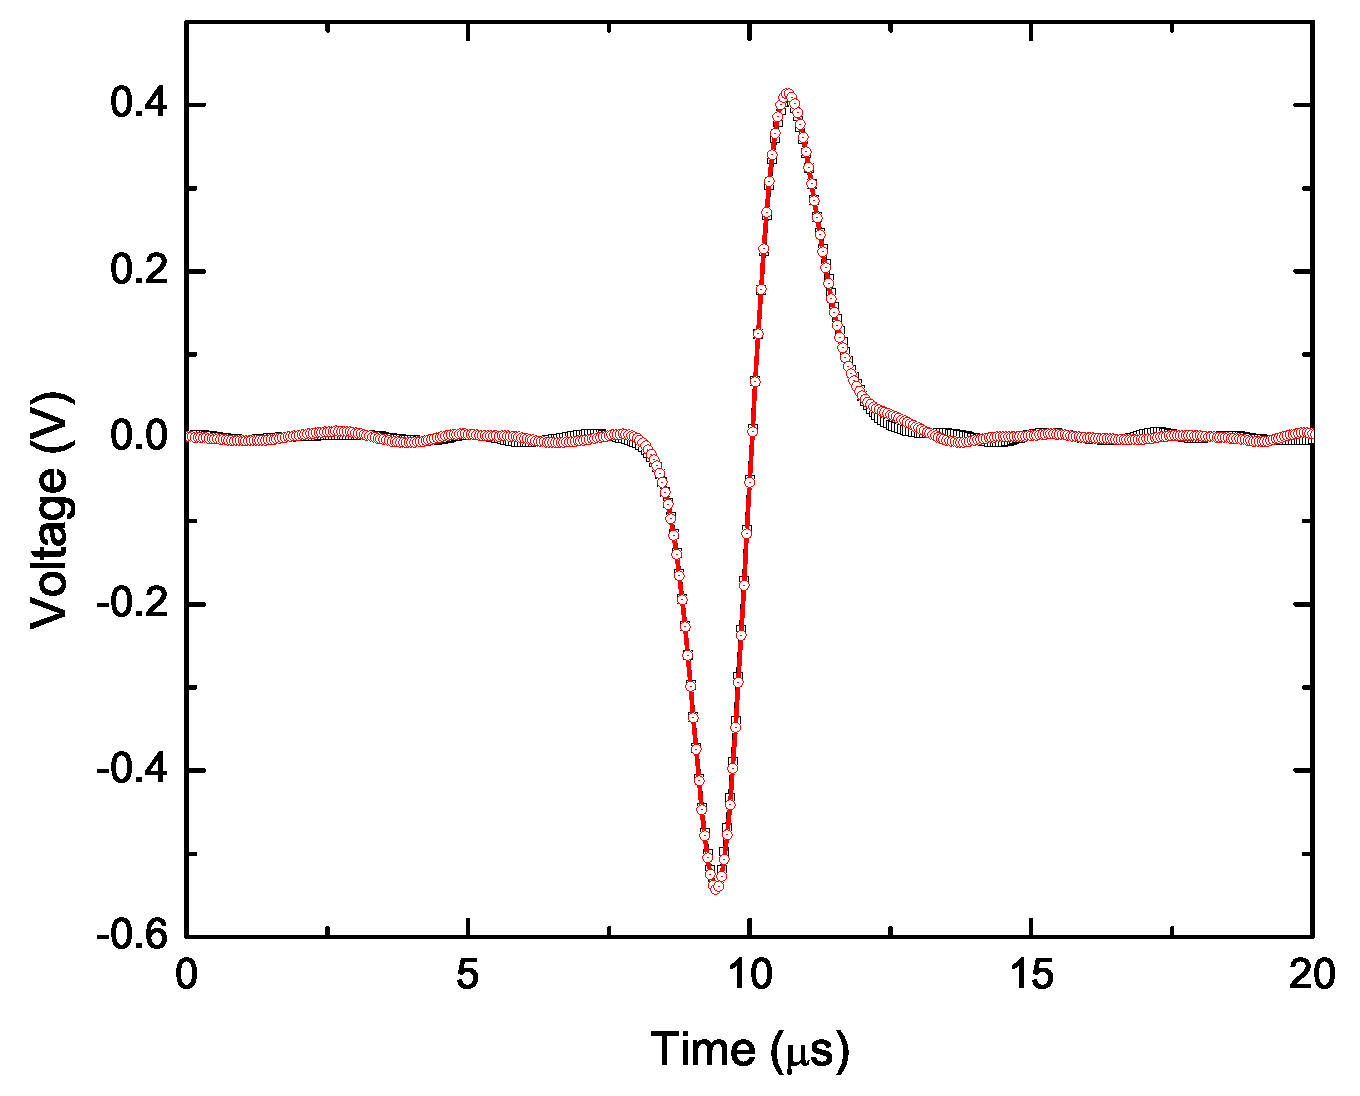
\includegraphics[width=0.7\linewidth]{AsFaradayCupBipolar}
	\caption{Bipolar output of the shaping amplifier. The peak-to-peak voltage is proportional to the total charge in the pulse. Two lines are plotted, both of which are the average of 1024 consecutive ion bunches. The peak-to-peak voltages agree, so the average charge has been determined quite accurately to be $1.17 \pm 0.02$~fC.\label{fig:AsFaradayCupBipolar}}
\end{figure}
Each line corresponds to the average over 1024 consecutive ion bunches. The experiment has been performed twice to get an idea of the reproducibility of the measurement. As it turns out, the two experiments agree very well, so that the charge for this experiment is determined to be $1.17 \pm 0.02$~fC.

Within ten minutes of the charge determination, a voltage difference is applied over the MCP plates, so that it will act as a charge multiplier again. The applied voltage at the front of the MCP is $V_{in}=-1550$~V, while the rear of the MCP is at $V_{out}=0$~V. The phosphor screen is at a positive voltage of $V_{ph}=1000$~V. Now, the  output voltage of the transimpedance amplifier is averaged over 1024 consecutive ion bunches and this measurement is performed twice. The results are plotted in figure \ref{fig:AsMCPslowamp}. 
\begin{figure}[tbh!]
	\centering
		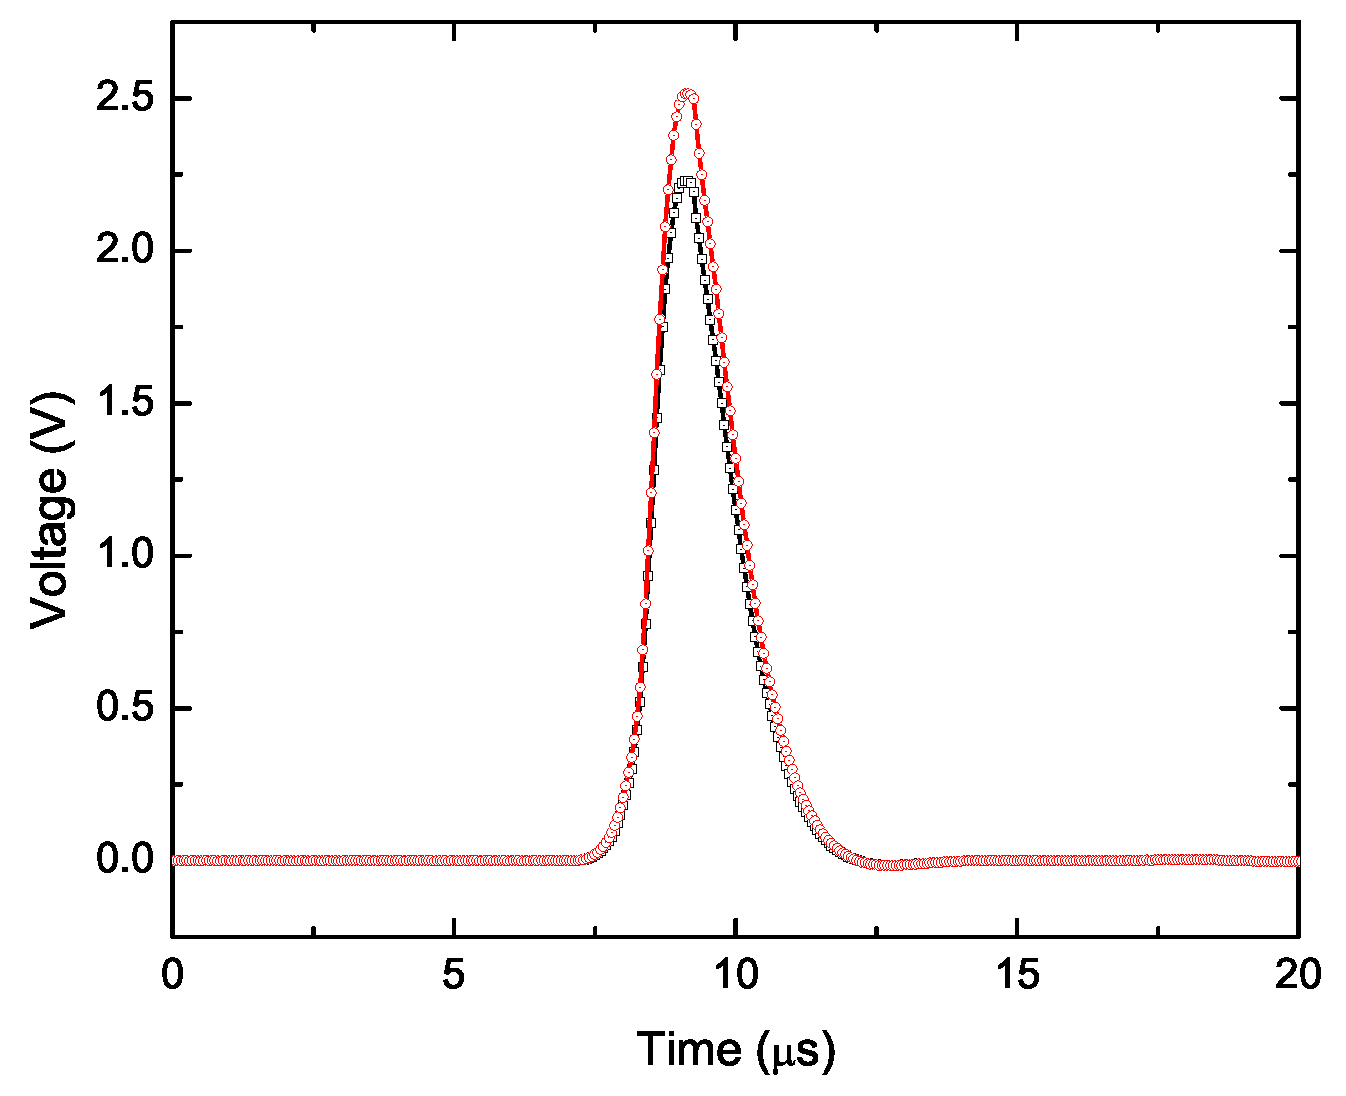
\includegraphics[width=0.7\linewidth]{AsMCPslowamp}
	\caption{The output of the trans-impedance amplifier, during the calibration measurement, where the different colors correspond to two identical series taken after each other. \label{fig:AsMCPslowamp}}
\end{figure}
In this case, there is some disagreement between the two measurements. This can be caused by a relatively small increase of the voltage over the MCP: a difference of only 7~V in terms of $\Delta_{MCP}=V_{out}-V_{in}$ could explain the change. This is in accordance with the voltage-stability of the high voltage supplies used to power the MCP. Hence, the minimal error margin of the current measurements is 10\%.
The signal needs to be integrated over time to get the charge of the bunch, which gives on average $(4.0 \pm 0.2)$~$\mu$V~s. This corresponds to a charge of $40 \pm 2$~pC and hence a MCP gain of $(34 \pm 2) \times 10^3$.

This calibration can be used to relatively calibrate the MCP for other acceleration voltages and MCP potential differences.
%In figures \ref{fig:CalibrationMCP1550Accell6kV} and \ref{fig:CalibrationMCP1550Accell800V}, the voltage on the output of the trans-impedance amplifier is plotted versus the time.
%\begin{figure}[tbh!]
%    \subfloat[$V_a=6$~kV]{
%        \label{fig:CalibrationMCP1550Accell6kV}
%        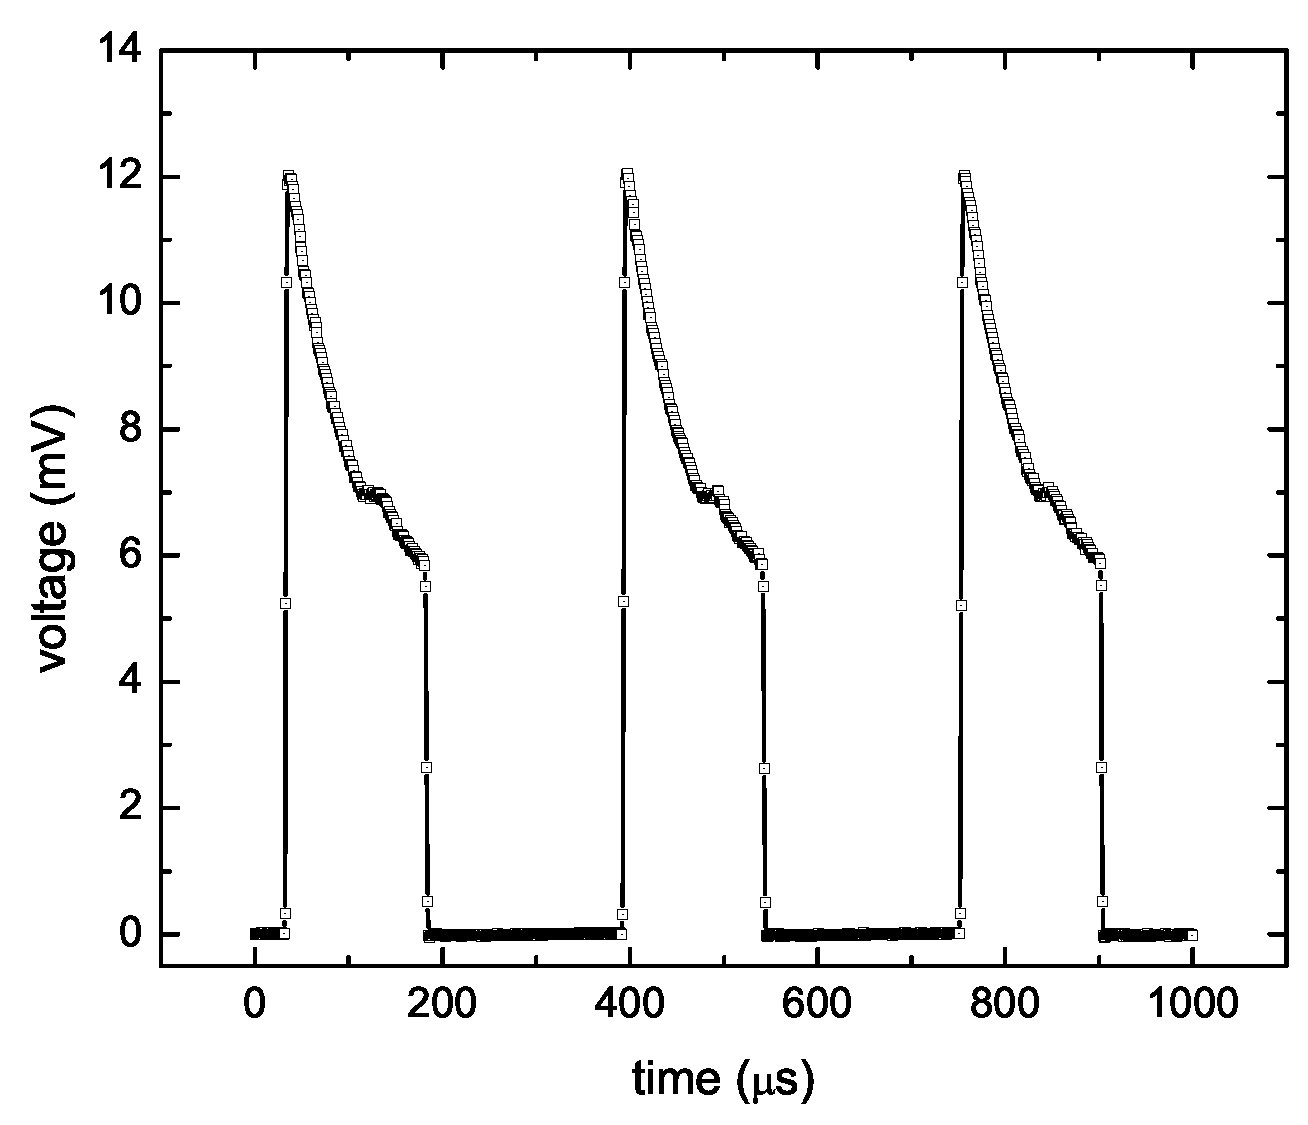
\includegraphics[width=0.48\linewidth]{CalibrationMCP1550Accell6kV}}
%    \hfill
%    \subfloat[$V_a=800$~V]{
%        \label{fig:CalibrationMCP1550Accell800V}
%        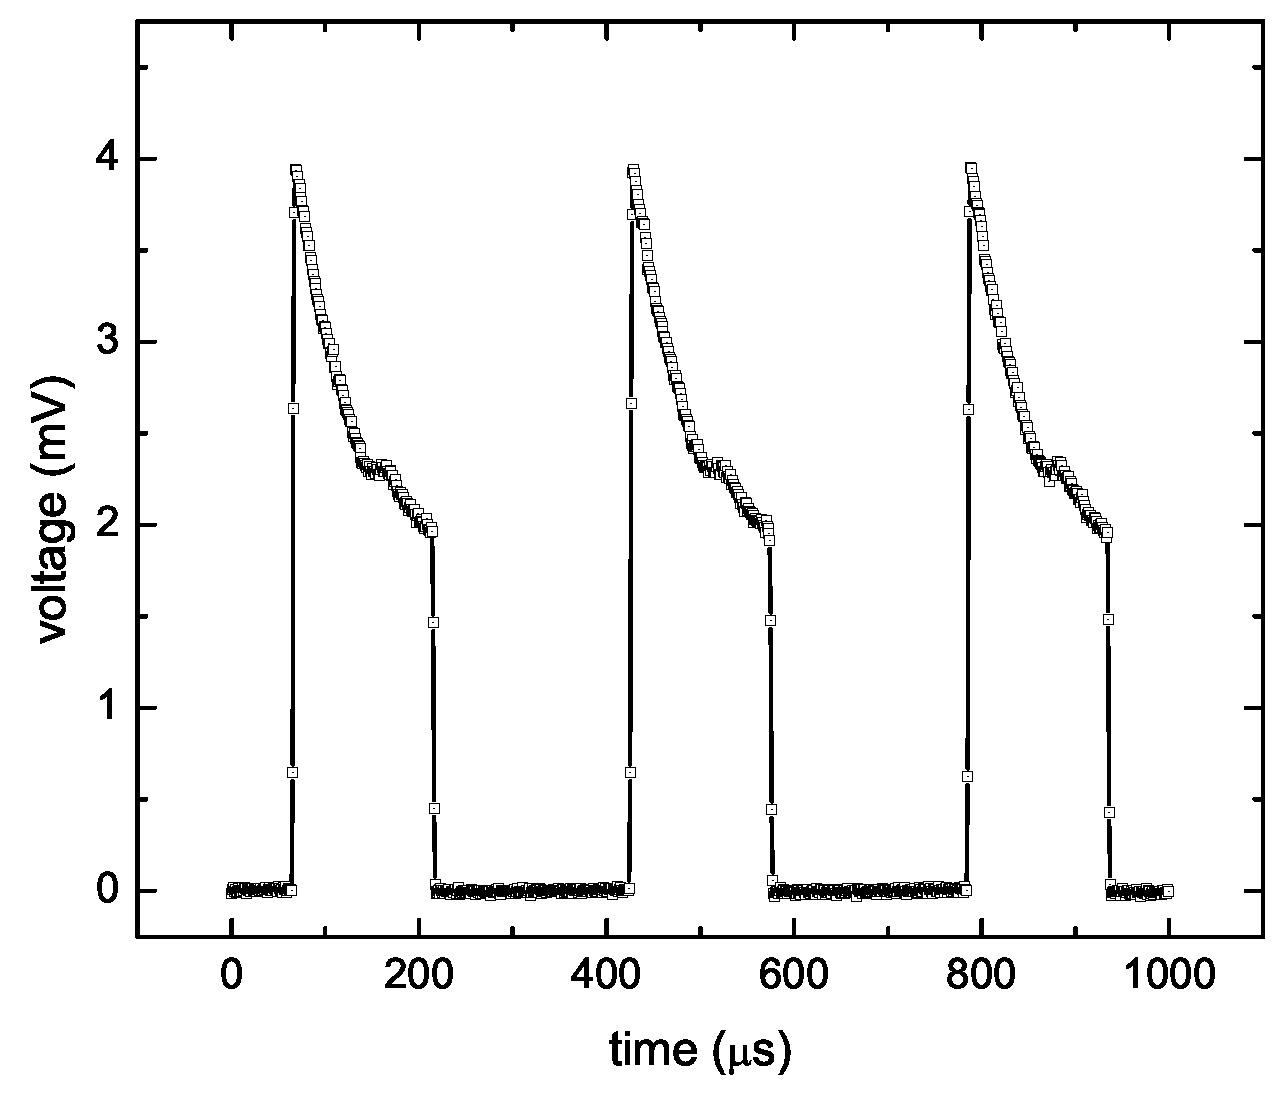
\includegraphics[width=0.48\linewidth]{CalibrationMCP1550Accell800V}}
%    \caption{Calibration experiment at an acceleration voltage of 6~kV and $\Delta_{MCP}=1550$~V, in panel (a). Panel (b) shows a calibration for an acceleration voltage of 800~V. The charge of the incoming ion bunches is determined by the integral of this signal.}
%    \label{fig:CalibrationMCP}
%\end{figure}
%In both figures, the plotted voltage is the average of 16384 ion bunches and they are performed with the same voltage over the MCP, namely $\Delta_{MCP}=1550$~V. The difference is the acceleration voltage, which is respectively 6~kV and 800~V. As can be seen, a lower acceleration voltage makes the time of flight for the ions longer, so that the measured current starts at a later time: the peak voltage is reached $32.5 \pm 0.5~\mu$s later. This is in good agreement with the expected value of $32.0~\mu$s, which can be obtained by assuming that the ions begin their acceleration exactly in the center of the MOT, accelerate for 1~cm to a kinetic energy corresponding to half the acceleration voltage, and travel at constant speed for 1.5~m. Another difference between the two figures is that the measured signal is weaker when a lower acceleration voltage is used. This can be explained by the quantum efficiency of the MCP, the probability that an electron is emitted when an ion hits the surface. If the ions arrive at higher energy, the quantum efficiency is typically higher, so on average more electrons will exit the MCP and hit the phosphor screen.
This is performed with $\Delta_{MCP}$ being 1500~V, 1600~V, 1650~V, 1700~V, 1750~V. The results of these experiments are plotted in figure \ref{fig:MCPcalibrationConstants}, which shows the gain of the MCP, plotted on a logarithmic scale, as a function of the voltage over the MCP, for an acceleration voltage $V_a=800$~V. 
\begin{figure}[tbh!]
	\centering
		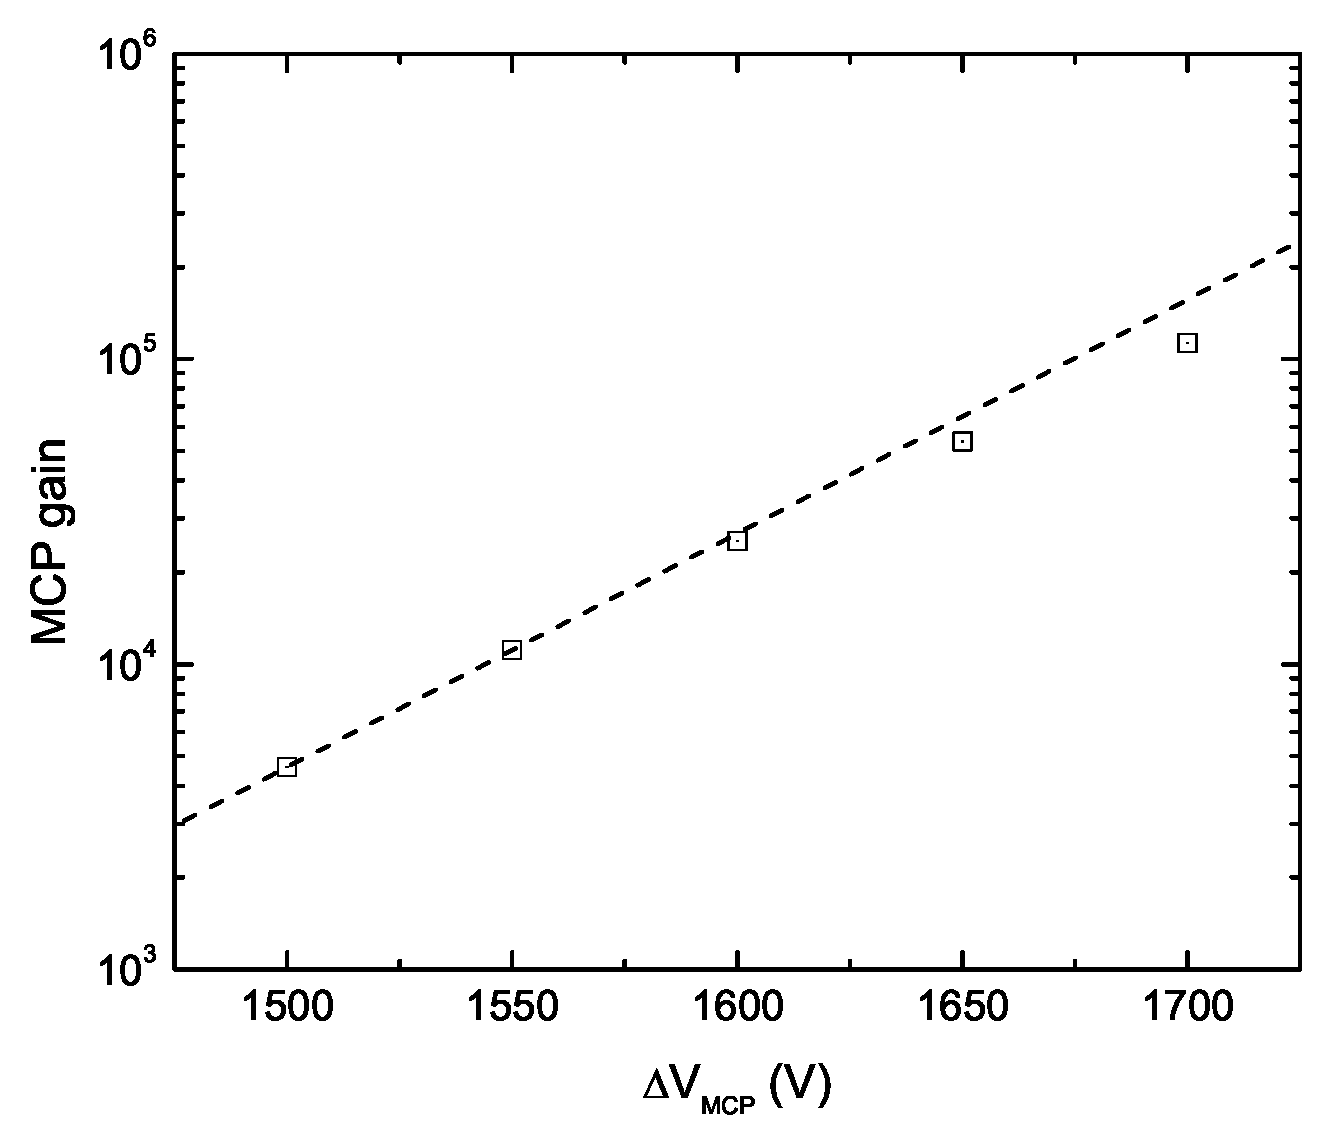
\includegraphics[width=0.7\linewidth]{MCPcalibrationConstants}
	\caption{The gain as determined by the calibration experiments for an acceleration energy $V_a=800$~V which correspond to a beam energy of about 400~eV. All points have a systematic error of about 10\%. The dashed line corresponds to an exponential increase of the gain, fitted through the first two points.\label{fig:MCPcalibrationConstants}}
\end{figure}
As can be seen the gain increases almost exponentially with the voltage. This exponential relationship (fitted through the first two points) has also been plotted as a dashed line. For higher voltages over the MCP a saturation effect occurs.

\section{Resolution of the MCP detector \label{sec:resoMCP}}
The resolution of the detector has been determined experimentally by placing two pinholes, with diameters $2 r_p$ of 25~$\mu$m and 50~$\mu$m, downstream in front of the MCP. This is important for the measurement presented in chapter 3. Ion bunches with $U = 3$ keV passed through one of the two pinholes at a time. The \textit{rms}-radius $\sigma_a$ of an aperture with radius $r_p$ is given by
\begin{equation}
     \sigma_a = \sqrt{\frac{\int dx~x^2\sqrt{r_p^2-x^2}}{\int dx\sqrt{r_p^2-x^2}}}=\frac{r_p}{2},
\end{equation}
The \textit{rms} spot radius $\sigma_{det}$ measured at the detector was substantially larger than $\sigma_a$, independently on the pinhole size used, as a result of the resolution of the detector. Figure \ref{fig:MCPresolution} shows one example obtained with the 25~$\mu$m pinhole, where a profile is fitted with a Gaussian. 
\begin{figure}[tbh!]
	\centering
		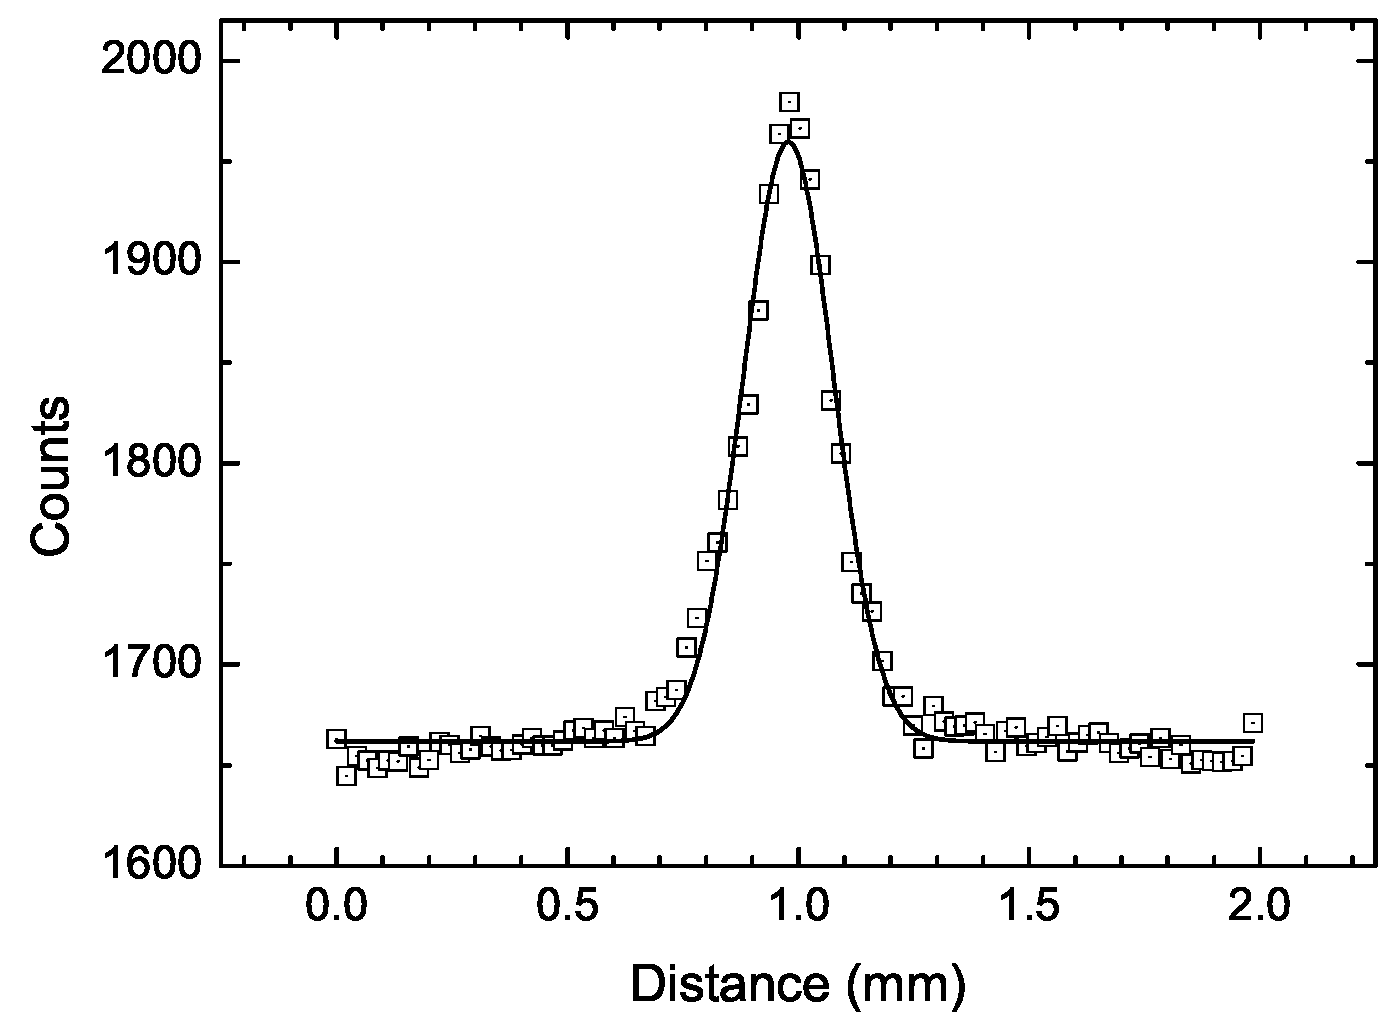
\includegraphics[width=0.7\linewidth]{MCPresolution}
	\caption{Plot profile of the spot size at the detector. The solid line is a Gaussian fit and it results in $\sigma_{det}=98~\mu$m.\label{fig:MCPresolution}}
\end{figure}
In this case, the $\sigma_{det}=98~\mu$m. Multiple experiments, with both the pinholes, have been performed in order to obtain sufficient statistical accuracy. Using
\begin{equation}
     \sigma_{det} = \sqrt{\delta^2 + \sigma_a^2},
\end{equation}
the \textit{rms} resolution of the detector $\delta$ is found to be $(95 \pm 4)$ $\mu$m.
\\


\bibliographystyle{unsrt}

\begin{thebibliography}{10}

\bibitem{Reijnders2010}
M.~P. Reijnders.
\newblock {\em Ion beams from laser-cooled gases}.
\newblock PhD thesis, Eindhoven University of Technology, 2010.

\bibitem{Taban2009}
G~Taban.
\newblock {\em A cold atom electron source}.
\newblock PhD thesis, Eindhoven University of Technology, 2009.

\bibitem{Metcalf_Book_99}
H.J. Metcalf and P.~van~der Straten.
\newblock {\em {L}aser {C}ooling and {T}rapping}.
\newblock Springer, 1999.

\bibitem{Claessens06}
B.~J. Claessens.
\newblock {\em Dynamics and Applications of Excited Cold Atoms}.
\newblock PhD thesis, Eindhoven Technological University, 2006.

\bibitem{Hermans10}
K.H.M. Hermans.
\newblock {\em Measurement and modeling of Ultra Cold Ion current pulses}.
  {Bachelor's thesis, Eindhoven Technological University}, 2010.
  
\bibitem{vdHeijden11}
M.A. van~der Heijden.
\newblock {\em Creation and characterization of ultrashort ultracold electron
  bunches}.
\newblock Master's thesis, Eindhoven Technological University, 2011.
  
\end{thebibliography}

\end{document}
 \chapter[Measurement of the temperature of an UCIS]{Measurement of the temperature of an ultracold ion source using time-dependent electric fields\label{ch:tempmea}}

%%\documentclass [10pt,a4paper] {article}
%\documentclass[aip,jap,twocolumn,reprint,showpacs,floatfix]{revtex4-1}
%%\documentclass[aip,jap,onecolumn,preprint,showpacs,floatfix]{revtex4-1}
%
%\providecommand{\e}[1]{\ensuremath{\times 10^{#1}}}
%\usepackage{graphicx}% Include figure files
%\usepackage{dcolumn}% Align table columns on decimal point1
%\usepackage{bm}% bold math
%\usepackage{subfigure}  % use for side-by-side figures
%
%\begin{document}
%
%%\title{Ultracold ion source temperature measurement with a time-dependent electric field}
%\title{Measurement of the temperature of an ultracold ion source using time-dependent electric fields}
%
%\author{N. Debernardi, M.P. Reijnders, W.J. Engelen, T.T.J. Clevis, P.H.A. Mutsaers, O.J. Luiten and E.J.D. Vredenbregt}
%\email{E.J.D.Vredenbregt@tue.nl}
%\affiliation{Department of Applied Physics, Eindhoven University of Technology, P.O Box 513, 5600 MB Eindhoven, the Netherlands}
%
%
%\date{\today{}}

\begin{abstract}
%The source temperature, $(1 \pm 2)$ mK, and the corresponding transversal reduced emittance, $7.9 \e{-9}$ m rad $\sqrt{eV}$, have been experimentally measured with a new and direct method. The effect of space charge has been studied at low energies (few tens of eV) and at ultra low average charge per bunch (0.02 ions per bunch). A new way to focus ion beams with time-dependent electric fields is presented in this paper.
We report on a measurement of the characteristic temperature of an ultracold rubidium ion source, in which a cloud of laser-cooled atoms is converted to ions by photo-ionization. Extracted ion pulses are focused on a detector with a pulsed-field technique. The resulting experimental spot sizes are compared to particle-tracking simulations, from which an effective source temperature $T = (3 \pm 2)$ mK and the corresponding transversal reduced emittance  $\epsilon_r = 1.4 \times 10^{-8}$ m rad $\sqrt{\rm{eV}}$ are determined. Space charge effects that may affect the measurement are also discussed. %We find that this result is likely limited by space charge forces even though the average number of ions per bunch is 0.022.
\footnote{The work described in this chapter (appendix excluded) is based on the article published by \underline{N. Debernardi}, M.P. Reijnders, W.J. Engelen, T.T.J. Clevis, P.H.A. Mutsaers, O.J. Luiten, and E.J.D. Vredenbregt in J. Appl. Phys. \textbf{110}, 024501 (2011).}
\end{abstract}

%\pacs{29.27.Bd, 32.80.Fb, 41.75.Ak, 67.85.-d}

%\maketitle
\clearpage

\section{Introduction}
Focused Ion Beams (FIBs) are widely utilized in the semiconductor industry and in nanoscience \cite{Orloff_Book_03, Orloff_RoSI_93}. They are used successfully for high precision milling or deposition and on the other hand, similarly to scanning electron microscopy (SEM), for high resolution microscopy \cite{Ward_JVSTB_06}. To keep up with reduction in sizes in the semiconductor industry it is necessary to reduce the smallest focusable spot size \cite{itrs, Moore_E_65}. The properties of the source have a key role in what can be achieved. A typical FIB using the current industry-standard Liquid Metal Ion source (LMIS) can reach a high brightness ($10^6$~A/m$^2$~sr~eV) and can deliver 10 pA current in 10 nm spot size \cite{Orloff_RoSI_93} (note that higher currents can be reached if the beam is less focused). Brightness is the current per unit area and solid angle, normalized by the beam energy and it is a key property for a source. A new kind of ion source, the ultracold ion source (UCIS) has been proposed as an alternative for the LMIS \cite{Hanssen_PRA_06, Geer_JoAP_07, Claessens_PoP_07}. The UCIS is based on creating very cold ion beams by near-threshold photo-ionization of a laser-cooled and trapped atomic gas, with a source temperature $T$ less than 1 mK. The UCIS has the potential of producing ion beams with a brightness of $10^5$~A/m$^2$~sr~eV and a current up to 100 pA, according to simulations \cite{Geer_JoAP_07}. Its major advantage is an energy spread two orders of magnitude lower than the LMIS (down to 10 meV) as demonstrated by Reijnders \textit{et al.} \cite{Reijnders_PRL_09}. Lower energy spread may lead to a smaller achievable spot size by reducing the contribution of chromatic aberration \cite{Geer_JoAP_07}.\\ %When the chromatic aberration is the dominant term, this could result a 0.8 nm spot size, with an usable current of 1 pA \cite{Geer_JoAP_07, Kruit_NL_08}.\\
This work aims to measure the source temperature of a rubidium UCIS, which is an important physical quantity related to the ability to focus the beam. Here we show how an effective source temperature can be extracted from measurements of the minimum spot size achieved in focusing the beam and we demonstrate a new way to focus ion beams. The ultra low temperature of the source permits collimated beams to be created at low energy (down to a few eV \cite{Reijnders_PRL_09}), which allows using time-dependent fields for accelerating and focusing. The duration and the shape of the accelerating electric field pulse can be tuned so that a variable focusing lens is created. An effective source temperature is then extracted from waist scans varying the focal strength of the time-dependent lens.


\section{Principle of the measurement}
\label{sec:prin}
In the experiment, ion bunches, extracted from the source with longitudinal energy $U$, are deposited on a detector with a variable focal length $f$. With a simple first order optical model it is possible to find an upper limit for the source temperature from the final root-mean-square (\textit{rms}) spot radius $\sigma_{x_f}$ (see figure \ref{fig:opt_model} for a schematic drawing), assuming that the emittance is conserved.
\begin{figure}[tbh!]
    \centering
        \includegraphics[width=0.7\linewidth]{pics/tempmea/opt_model3.eps}
    \caption{Principle of the source temperature measurement. Ion bunches are focused on a detector with a time-dependent lens with focal length $f$. The quantity $\sigma_{x'_i}$ is the initial \textit{rms} angular spread, $\sigma_{x_i}$ is the initial \textit{rms} radius of the source and $\sigma_{x_f}$ the \textit{rms} radius of the final spot on the detector.}
    \label{fig:opt_model}
\end{figure}

The size of the ion bunch at the detector position is completely determined by the initial \textit{rms} angular spread $\sigma_{x'_i}$ when the focal distance length of the (thin) lens corresponds to the distance between the lens and the detector,
\begin{equation}
    \sigma_{x_f} = f \sigma_{x'_1}.
    \label{eq:angSpread}
\end{equation}
The \textit{rms} value of the angular spread is related to the source temperature $T$ by
\begin{equation}
    \sigma_{x'_i} = \sqrt{\frac{k_b T}{2U}},
    \label{eq:spread}
\end{equation}
where $k_b$ is Boltzmann`s constant and $U$ is the energy of the bunch. 
Reversing this equation, the source temperature can be defined given a measurement of $\sigma_{x_f}$ as
\begin{equation}
    T = \frac{2}{k_b} U \left(\frac{\sigma_{x_f}}{f}\right)^2.
    \label{eqT}
\end{equation} 
Any emittance growth, e.g., due to distortions in the imaging system, will affect the extracted value of $T$, which thus becomes an effective source temperature.
Knowing $T$ and thus $\sigma_{x'_i}$, we can derive the \textit{rms} normalized emittance $\epsilon_r$ of the source when, in addition, the source radius $\sigma_{x_i}$ is known. The normalized emittance is a measure of the phase space occupied by the beam multiplied by the square root of the beam energy and is given by \cite{Luiten_IJoMPA_07}
\begin{equation}
    \epsilon_r = \sigma_{x_i} \sigma_{x_f} \sqrt{U} = \sigma_{x_i} \sqrt{\frac{k_b T}{2}}.
    \label{eq:emitt2}
\end{equation}
Indeed in equation (\ref{eq:emitt2}) the dependence on the energy $U$ disappears indicating that the normalized emittance is a property of the source.


\section{Experimental Setup}
\label{sec:setup}
The UCIS is based on the technique of laser cooling and trapping of neutral atoms \cite{Metcalf_Book_99, Foot_Book_05}. We start with a magneto-optical trap (MOT) of rubidium atoms. Three orthogonal pairs of counter propagating 780 nm laser beams (trapping laser beams) are used to Doppler cool a $^{85}$Rb atomic cloud and a quadrupole magnetic field is added to trap the atoms. Typically $10^8$ Rb-atoms are trapped in a volume of  16~mm$^3$ \textit{rms} at an expected source temperature of $T_0=~143~\mu$K \cite{Metcalf_Book_99}, which corresponds to 9~neV of average kinetic energy of the atoms. The MOT is surrounded by an accelerator \cite{Taban_PRSAB_08}.\\
The accelerator has a cylindrically symmetric structure and it is placed in a vacuum chamber where the rubidium pressure is $10^{-9}$ mbar. See figure \ref{fig:setup_curr} for a schematic drawing of the experimental setup. The trapping laser beams enter through openings present in the structure. The atomic cloud is trapped in the middle of the accelerator at the intersection of the trapping laser beams, 10 mm away from the accelerator's exit, which consists of a circular hole with a diameter of 20 mm. The electric field strength at the starting point $z_0$ is 0.37 kV/cm per kV input voltage $V_a$ and $U = e V_a/2.05$, where $e$ is the elementary charge. For details of the accelerator structure see \cite{Taban_PRSAB_08}.
\begin{figure}[tbh!]
    \centering
        \includegraphics[width=0.7\linewidth]{pics/tempmea/setup.eps}
    \caption{Schematic view of the experimental setup (not to scale) in the x-z plane. The ionization laser beam and the excitation laser beam select a portion of the Rb atomic cloud trapped inside the accelerator. The bunched ions are accelerated using a time-dependent potential $V_a (t)$ and after a flight distance of 1.51 m they reach a MCP detector with a phosphor screen. The images are captured by a CCD camera.}
    \label{fig:setup_curr}
\end{figure}

The ionization mechanism is a 2-step process. In order to avoid spherical aberration in the focusing process, it is necessary to work with a smaller volume than the total MOT. To achieve this, the trapping laser beams are turned off for 25 $\mu$s (the MOT magnetic field is turned on all time). During this time, a laser beam (excitation laser beam) with the same wavelength (780 nm) is focused horizontally along the z-direction to a \textit{rms} radius $\sigma_{excit} = 54$ $\mu$m. The excitation laser beam excites the Rb cloud to the 5p-level for 2 $\mu$s. Coincidentally, a 479 nm ionization laser beam is sent in vertically along the x-direction for 400 ns. The ionization laser beam also has an \textit{rms} radius $\sigma_{ioniz} = 54$ $\mu$m. Figure \ref{fig:timings} shows an experimental example of the timing sequence used for the ionization of a portion of the Rb atomic cloud trapped in the MOT.
\begin{figure}[tbh!]
    \centering
        \includegraphics[width=0.6\linewidth]{pics/tempmea/timings.eps}
    \caption{Typical example of the timings used in the experiment to ionize a portion of the whole atomic cloud. The trapping laser beams are turned off
for about 25 $\mu$s and during this time the excitation and ionization laser beams are turned on in coincidence. The excitation laser beam is turned on for 2 $\mu$s and the ionization laser beam for 400 ns.}
  \label{fig:timings}
\end{figure}
In this way, only the atoms at the intersection of the 2 laser beams will be ionized. The shape and position of the ionized cloud can be changed by changing the size of the lasers and their position. The position and dimension of the lasers are controlled by 2 CCD cameras, virtually positioned in the center of the MOT, which is at $z_0$ on the beam axis. The initial ionization volume is not spherical: in the x-direction the \textit{rms} radius $\sigma_x$ is determined by the intersection of two laser beams and hence
\begin{equation}
     \frac{1}{\sigma_x} = \sqrt{\frac{1}{{\sigma_{excit}}^2} + \frac{1}{{\sigma_{ioniz}}^2}},
\end{equation}
so that $\sigma_x$ is a factor $\sqrt{2}$ smaller than the size of the two laser beams.\\
The initial ionization volume size has been experimentally and numerically determined as follows. Ion bunches are created in a DC electric field and are consequentially accelerated towards the detector (which is described below). With a DC accelerating field, the exit of the accelerator forms an aperture lens with a negative focal length $f_0$ of 33~mm (``exit kick'' effect), which is independent of the acceleration voltage \cite{Taban_PRSAB_08}. This leads to a magnified image of the source on the detector with a known magnification of 46. From the final spot size, it is therefore possible to determine the source size. The initial angular spread has a negligible influence (less than $1\%$) on the final spot size for $U > 200$ eV and this measurement was performed at $U=3$~keV. The initial volume is assumed to be Gaussian distributed in all 3 directions from the fact that the profile of the lasers is Gaussian as well. Analysis of the recorded detector images give $\sigma_x =$ (38 $\pm$ 2) $\mu$m and $\sigma_y =$ (54 $\pm$ 3) $\mu$m. In the z-direction, $\sigma_z =$ 54 $\mu$m because it equals the \textit{rms} radius of the ionization laser beam $\sigma_{ioniz}$.\\
A double multichannel plate (MPC) detector with phosphor screen is located at 1.51 m from the ion's starting position $z_0$. The diameter of the MCP is 40 mm. A 16 bit, cooled CCD camera is used to image the phosphor screen through a lens placed in between with a magnification of 0.33. The spatial distribution of the ion bunches can be extracted from the CCD images. The resolution of the detector has been determined experimentally by placing two pinholes, with diameters of 25 $\mu$m and 50 $\mu$m, downstream in front of the MCP. Ion bunches with $U = 3$ keV passed through the pinhole. The \textit{rms} radius $\sigma_a$ of an aperture with diameter $D$ is equal to $D/4$. The \textit{rms} spot radius $\sigma_{det}$ measured at the detector was substantially larger than $\sigma_a$, as a result of the resolution of the detector. Multiple experiments, with both the pinholes, have been performed in order to obtain sufficient statistical accuracy. Using
\begin{equation}
     \sigma_{det} = \sqrt{\delta^2 + \sigma_a^2},
\end{equation}
the \textit{rms} resolution of the detector $\delta$ is found to be $(95 \pm 4)$ $\mu$m. In what follows, $\delta$ is quadratically subtracted from the measured spot in order to obtain $\sigma_{x_f} = \sqrt{\sigma_{det}^2 - \delta^2}$.


\section{Focusing with time-dependent electric fields}
Measuring the effective temperature of the source requires focusing the ion bunches onto the detector. In fact, as described in section \ref{sec:prin}, at the beam waist the final spot size is completely determined by the initial angular transverse spread, which depends on the source temperature. To focus the ions, a positive lens is required, while the aperture lens formed by the accelerator is negative. However, the sign can be reversed using time-dependent accelerating fields. Due to the low temperature of the ions, it is possible to form well-collimated ion beams at very low energies, $U \approx 10-50$ eV. Such ions travel for few microseconds in the accelerator before exiting it. For instance, in the case of $U= 30$ eV, the traveling time is in the order of 3 $\mu$s. This time is long enough to switch the accelerating field while the ions are still in the accelerator.\\
When a constant positive voltage is applied to the anode the ions will experience a negative lens effect. The on-axis longitudinal electric field $E_z(z)$ follows approximately a Gaussian centered on $z_0$, see figure \ref{fig:fields}b.
\begin{figure}[tbh!]
    \centering
        \includegraphics[width=0.7\linewidth]{pics/tempmea/fields2.eps}
    \caption{The potential applied to the anode $V_a$, the longitudinal electric field component $E_z$ and the radial electric field component $E_r$ (for $r \neq 0$), in case of a static (left hand side) or bipolar field (right hand side). The quantities $\tau_p$ and $z_s$ are the length respectively in time and space of the positive part of the pulse. In panels (d), (e) and (f), the thin line indicates the static case. The y-axis is in arbitrary unit in all the six
plots.}
    \label{fig:fields}
\end{figure}
Figure \ref{fig:fields} shows the potential applied to the anode $V_a(t)$, the longitudinal electric field component along the beam axis $E_z(z)$ and on-axis radial electric field component $E_r(z)$ for $r \neq 0$, in case of a static (left hand side) or bipolar field (right hand side).
The cylindrical symmetry of the accelerator makes it possible to write the electric field in the accelerator as an expansion of the electric field on the symmetry axis. In a first order approximation, the radial electric field component $E_r(r,z)$ is given by
\begin{equation}
    E_r(r,z) = -\frac{r}{2} \frac{dE_z}{dz},
\end{equation}
where $r$ is the radial position. In the case of a static electric field, the focal strength of the accelerator is described by
\begin{equation}
   \frac{1}{f_0} = - \frac{1}{4} e_z(z_0),
   \label{eq:f_DC}
\end{equation}
where $f_0$ is the time-independent focal length, and the static field  $e_z(z) = E_z(z) / \phi_0$, with the potential given by $\phi_0 = \int_{z_0}^\infty E_z(z') dz'$, as suggested in \cite{Reijnders_JAP_11}. Because the integral of the radial electric field experienced by an ion over time is positive (see figure \ref{fig:fields}c in dark), a defocussing effect results.\\
By turning off the electric field before the ions leave the accelerator one can cancel the exit kick effect. Moreover, with the use of a bipolar pulse, the exit kick effect can be reversed and a focusing lens created, see figure \ref{fig:fields}f. In this case, the net integral of the radial electric field component will then result to be negative. Typically the electric fields can be changed in less than 100 ns. Bipolar pulses are created with a programmable waveform generator and amplified 50 times. An example of a bipolar pulse $V_a(t)$ used in the experiment can be seen in figure \ref{FIG:pulse}.
\begin{figure}[tbh!]
    \centering
        \includegraphics[width=0.7\linewidth]{pics/tempmea/pulse.eps}
    \caption{Example of a typical bipolar anode voltage pulse $V_a$ used in the experiment. Here, $V_{pos} = 125$ V is the positive voltage with duration $\tau_p=2$ $\mu$s and $V_{neg}= -90$ V is the negative voltage with duration $\tau_n=4$ $\mu$s. The pulse is created with a programmable waveform generator, amplified 50 times and applied to the accelerator.}
    \label{FIG:pulse}
\end{figure}
Here we can define the positive voltage $V_{pos}$ with duration $\tau_p$ and the negative voltage $V_{neg}$ with a duration $\tau_n$ long enough in order that the ions have already left the accelerator when $V_a$ goes to zero. The accelerating pulse is turned on within 100 ns after the ionization laser is off. The ion bunch moves downstream in the direction of the detector (see figure \ref{fig:setup_curr}).\\
Now a ``waist scan'' can be performed, i.e. the final spot size is measured depending on one of these parameters. What is actually varied then is the focal strength $1/{f_t}$, which in the case of a bipolar pulse, can be expressed as
\begin{equation}\label{eq:f_bip}
	\frac{1}{f_t}  = \frac{1}{f_0} + \frac{V_{pos} - |V_{neg}|}{4 V_{pos}} e_z(z_s).
\end{equation}
Here, $z_s$ is the position to which the center of the ion bunch has moved when the field is switched from positive to negative (at time $\tau_p$). Obviously, the focal strength depends on $V_{pos}$, $V_{neg}$ and $\tau_p$, not only directly but also through their influence on $z_s$. In the experiment we only vary $V_{neg}$, for a fixed $V_{pos}$ and $\tau_p$. The bunch energy is given by
\begin{equation}\label{eq:en}
U=e \int_{z_0}^\infty{E_z dz}.
\end{equation}
It is of interest to note that $U$ varies during a waist scan due to the different values of $V_{neg}$.\\
For further details about focusing with time dependent fields see Reijnders \textit{et al.} \cite{Reijnders_JAP_11}.


\section{Analysis}
\label{sec:ana}
Images collected from the CCD camera are fitted to a 2-dimensional Gaussian. Due to the fact that the initial volume is not spherical (see section \ref{sec:setup}), this will result in a non-circular spot on the images. The longer size is by definition in the y-direction and the short size is in the x-direction. Only the x-direction is considered in this paper because along y-direction the bunch suffered from aberrations, which we ascribe to the long beam line and low energy of the ions, which makes them particularly sensitive to small external fields. In the x-direction, residual effects cannot be completely excluded, in which case the extracted temperature will effectively include such distortions, which will generally increase the source emittance.

Particle tracking simulations have been performed with the General Particle Tracer code (GPT) \cite{gpt} in order to reproduce the measurements and fit the data. The electric field inside the accelerator has been calculated with the Superfish Poisson solver \cite{Halbach_PA_76}. The initial particle distribution is a 3D Gaussian with dimensions $\sigma_x$, $\sigma_y$ and $\sigma_z$ as listed in section \ref{sec:setup}, centered at position $z_0$. The initial velocities follow a Boltzmann distribution. A time-dependent $V_a(t)$ is applied depending on parameters varied experimentally, e.g. $V_{neg}$. The \textit{rms} radius of the simulated images are calculated and compared to the experimental data. Minimization of the reduced $\chi^2$ is performed when comparing the measurement data with GPT simulations in order to extract a parameter such as the effective source temperature. According to \cite{Bevington_Book_03}, the accuracy $\sigma_p$ of the parameter that is optimized by minimizing the $\chi^2$ can be calculated from the dependence of $\chi^2$ on that parameter in the region of the minimum as
\begin{equation}
    \sigma_p = \sqrt{2\left(\frac{\partial^2\chi^2}{\partial p^2}\right)^{-1}}.
\end{equation}


\section{Results and discussion}
The measurements presented here consist of waist scans where the negative voltage of the time-dependent pulse $V_{neg}$ has been varied. Because of the change of $V_{neg}$, the focal strength of the time-dependent lens varies, as shown in equation (\ref{eq:f_bip}). The other parameters are fixed: $\tau_p = 2$ $\mu$s, $\tau_n =$ 4 $\mu$s (see figure \ref{FIG:pulse}) and $V_{pos} =$ 125 V (except in the measurement in figure \ref{fig:diffEn}, where this parameter is also varied).\\
The repetition rate during all the experiments is 20 kHz and the exposure time of the CCD is 2 s. Thus every image is the sum of 40000 bunches.

\subsection{Temperature determination} \label{sec:Test}
Figure \ref{fig:diffEn} presents four waist scans at four different $V_{pos}$.
\begin{figure}[tbh!]
    \centering
        \includegraphics[width=0.7\linewidth]{pics/tempmea/diff_low_en.eps}
    \caption{Spot radius $\sigma_{x_f}$ versus negative pulse amplitude $V_{neg}$ for 4 different $V_{pos}$ (indicated in the figure). The bunch energy $U$ at the minimum of the waist scan (which depends on $V_{pos}$ and $V_{neg}$) is also indicated in the label and varies from 14 eV to 34 eV.}
    \label{fig:diffEn}
\end{figure}
For each $V_{pos}$, the minimum spot radius occurs at different $V_{neg}$, and according to equation (\ref{eq:en}) also at a different beam energy $U$. The plot shows that the minimum spot radius $\sigma_{x_f}$ increases when $U$ is lowered: lower energy means longer time of flight and this results in a larger final spot radius. This also indicates that the measurement is indeed sensitive to the effective source temperature. To find $T$, first the minimum spot radius is calculated by fitting the bottom part of a waist with a second order polynomial. The extracted minimum spot radius squared $\sigma_{x_f}^2$ is plotted versus $U^{-1}$ in figure \ref{fig:Tdiffen}.
\begin{figure}[tbh!]
    \centering
        \includegraphics[width=0.7\linewidth]{pics/tempmea/Textraction_with_error.eps}
    \caption{Final spot radius squared $\sigma^2_{x_f}$ versus the reciprocal of the bunch energy $1/U$. The thick line is a linear fit, whose slope is proportional to the effective source temperature $T$.}
    \label{fig:Tdiffen}
\end{figure}
According to equation (\ref{eqT}), the temperature $T$ can be extracted from a linear fit. The effective source temperature is found to be $T = (4.9 \pm 0.3)$ mK. This temperature, while it is extremely low, is still rather high compared to the expected source temperature ($T_0=143$ $\mu$K), even when $T_0$ is corrected for the fact that the ionization laser beam was turned 0.6 nm above the ionization threshold. In fact, this would make $T_0'=390~\mu$K, because from the conservation of the energy theorem and due to the large difference in mass between electrons and ions, the ions temperature increases about 400~$\mu$m/nm and the electrons temperature of about 60~K/nm, intended for every nanometer of detuning above threshold.

To minimize any effect of space-charge forces on the effective source temperature, we analyzed in detail a waist scan obtained at en even smaller charge of about 0.022 ions per bunch (on average). The data is shown in figure \ref{fig:s27_GPT}.
\begin{figure}[tbh!]
    \centering
        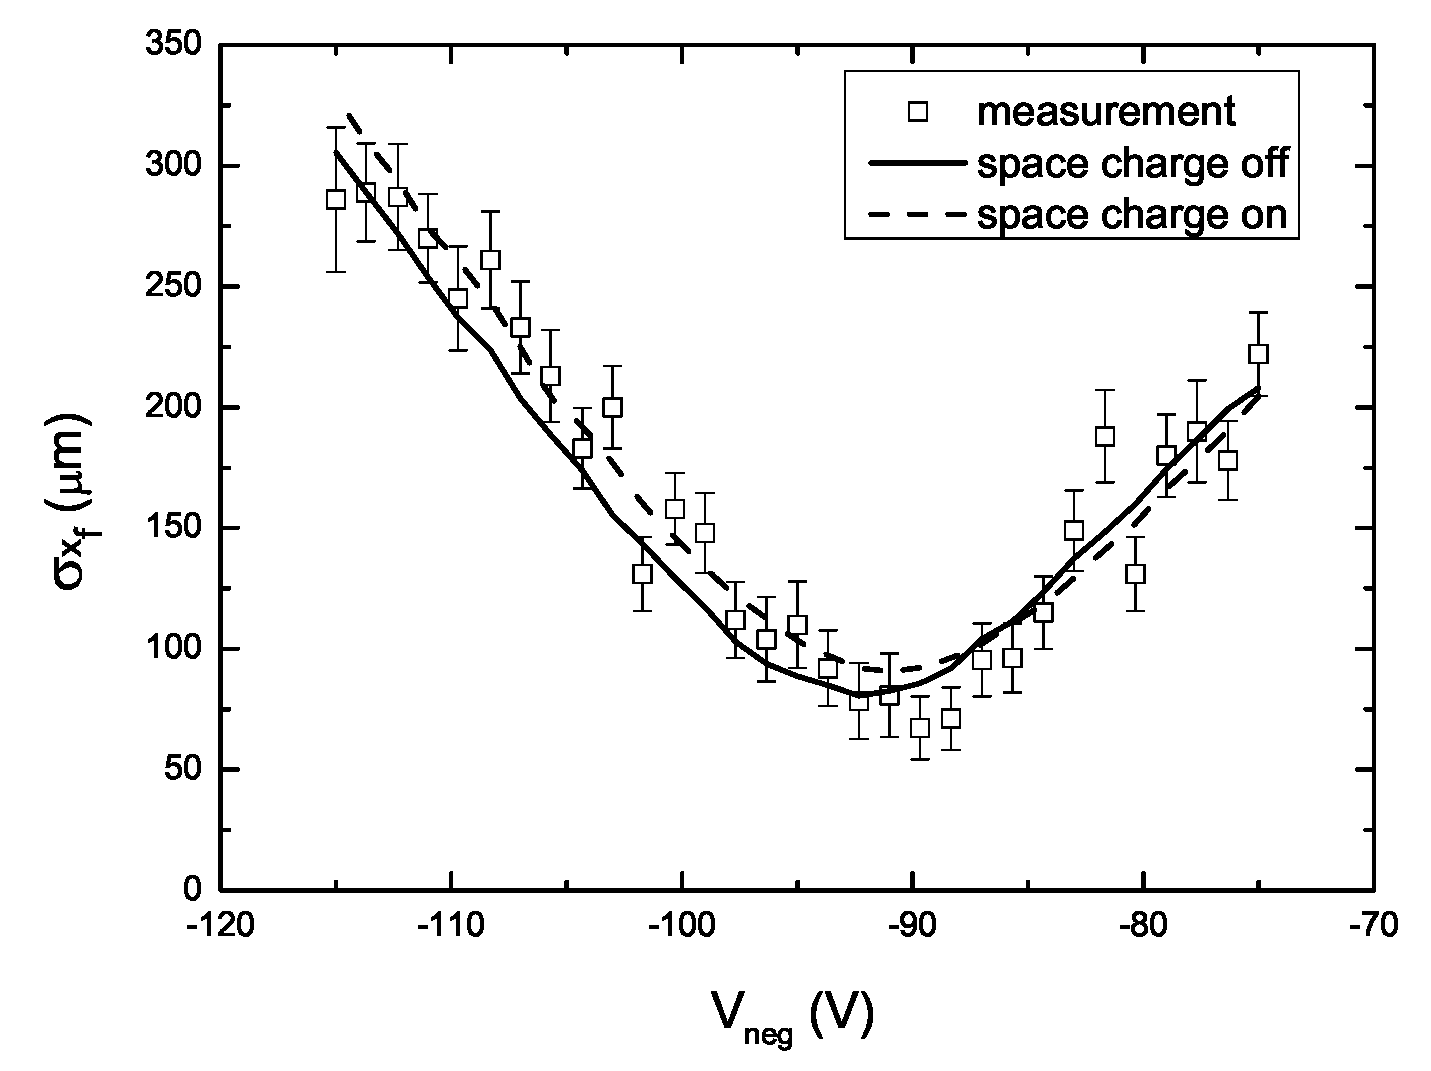
\includegraphics[width=0.7\linewidth]{pics/tempmea/s27_GPTfit_new.eps}
    \caption{Waist scan performed measuring the final spot size $\sigma_{x_f}$ versus the negative voltage of the time-dependent electric field $V_{neg}$. The experimental data is scattered with the error bars. The solid and the dashed lines are two GPT fits which do and do not include space charge forces respectively.}
    \label{fig:s27_GPT}
\end{figure}
The effective source temperature can be immediately estimated from equation (\ref{eqT}), as done in the previous paragraph. Using $U= 32$ eV (the bunch energy at the minimum position) and $\sigma_{x_f} = (73 \pm 4)$ $\mu$m, we find that the resulting effective source temperature $T= (1.8 \pm 0.2)$ mK. This first order approximation is confirmed by a fitting procedure, where the effective source temperature can be extracted more precisely by fitting the behavior of $\sigma_{x_f}$ versus $V_{neg}$ (figure \ref{fig:s27_GPT}) with particle tracking simulations. Waist scans are simulated for several source temperatures and the $\chi^2$-minimization procedure from section \ref{sec:ana} is applied. Figure \ref{fig:s27_GPT} shows a GPT simulation with parameters that best minimize the $\chi^2$ for different T (solid line). The extracted value is $T = (3 \pm 2)$ mK. The value of $\chi^2 = 1.5$ indicates that the model describe well the data but could be further improved. The uncertainty on the measurement is one standard deviation. %These GPT simulations do not include space charge, which might still be a limiting factor for the source temperature. The measurement shown in Fig. \ref{fig:s27_GPT} are performed with a 4 times smaller charge than the ones shown in Fig. \ref{fig:diffEn} and they result indeed in a lower source temperature. 
%In the next section, we investigate the eventual influence of space charge on the source temperature.\\


\subsection{Influence of space charge}
The measurements of figure \ref{fig:s27_GPT} were taken using far less than one ion per bunch and high repetition rate. Therefore, space charge forces should not be important in this case; but it is nevertheless interesting to investigate at which level Coulomb interactions can still play a role. The number of ions which are ionized by a laser beam follows Poissonian statistics, so it is possible, even when the expected average number of ions per bunch $\mu$ is less than one, to have some bunches with 2 or more ions. The Poisson distribution is given by $p_n(\mu,n) = (\mu^n e^{-\mu}/n!)$, where $n$ indicates the number of ions per bunch. As an example, when the expected number of ions per bunch is 0.022, the probabilities to obtain one, two or three ions per bunch are respectively 1.96\%, 0.02\% and 0.0001\%. The probability for zero ions is the highest (about 98\%) since only one ionization laser pulse every 50 ionizes one or more atoms. GPT simulations for $n>1$ show a dramatic increase of the spot size due to the low energy of the bunches. This is illustrated in figure \ref{fig:spots}, where the simulated distribution at the detector is shown for $n=1$, $n=2$ and $n=3$ at a bunch energy of 32 eV. The \textit{rms} radius for $n = 1,2,3$ in the x-direction is respectively $\sigma_1 = 65~\mu$m, $\sigma_2 = 471~\mu$m and $\sigma_3 = 635~\mu$m. The spot size due to $n=2$ and $n=3$ is much larger than the spot size due to $n=1$ and even if the probabilities for $n=2,3$ are low compared to that for $n=1$ they may play a role in the final spot size. The asymmetry present in the spots of figure \ref{n2} and \ref{n3} is due to the fact that the initial ionization volume is not spherical ($\sigma_x < \sigma_y$). In case of three particles per bunch, this effect is still noticeable but more smeared out, see figure \ref{n3}.
\begin{figure}[tbh!]
    \centering
    \subfloat[$n = 1$]{
        \label{n1}
        \includegraphics[width=0.28\linewidth]{pics/tempmea/n1.eps}}
    \hspace{.1in}
    \subfloat[$n = 2$]{
        \label{n2}
        \includegraphics[width=0.28\linewidth]{pics/tempmea/n2.eps}}
    \hspace{.1in}
    \subfloat[$n = 3$]{
        \label{n3}
        \includegraphics[width=0.28\linewidth]{pics/tempmea/n3.eps}}
    \caption{Particle distribution on the detector in GPT simulations depending on the number of ions in the bunch $n$. The plots are 2D histograms. The scale is the same in the three images: 3.2 by 3.2 mm$^2$. The horizontal axis is the x direction and the vertical axis is the y direction. The \textit{rms} radius for $n = 1,2,3$ in the x-direction is respectively $\sigma_1 = 65$ $\mu$m, $\sigma_2 = 471$ $\mu$m and $\sigma_3 = 635$ $\mu$m. The absolute number of counts per pixel is not of interest here and it is not given but the color code ranges from white (no count) to black (maximum number of counts). The asymmetry present in the spot size is due to the fact that the initial ionization volume is not symmetric.}
    \label{fig:spots}
\end{figure}

The sum distribution $D(x)$ is given by:
\begin{equation}
    D(x)=\sum_{n=1}^3{n p_n(\mu,n) D_n(x)},
    \label{eq:sum_distr}
\end{equation}
where $D_n(x)$ is the distribution of the final spot for $n= 1,2,3$ obtained from GPT simulations and $p_n$ is the Poisson probability used as a weight. The sum distribution is fitted to a 2-dimensional Gaussian. The standard deviation $\sigma_{sim}$ of the fitted Gaussian along the x-direction at different $V_{neg}$ is also showed in figure \ref{fig:s27_GPT} (dashed line). We find that space-charge forces have a very small effect on the waist-scan. The dashed line in figure \ref{fig:s27_GPT}, drawn for an effective source temperature of 3 mK, marginally improves the match with the experimental data ($\chi^2 = 1.1$). %seems to represent better the experimental data and it leads to a smaller source temperature of 1 mK, but also leads to a temperature uncertainty on the order of 1 mK.\\
While noticeable, it is uncertain if the resulting broadening can be actually extracted from the data since it is on the order of the accuracy of the measurement. Further investigations are required in order to quantify the influence of space charge.

%For $\mu = 0.022$ we obtain $\chi^2 = 1$. An average number of ions per bunch of 0.022 is not unrealistic. This number of ions can be obtained with a 400 ns long ionization laser beam pulse irradiating the considered initial volume assuming a atomic density of 10$^{14}$ atoms m$^{-3}$, which then contains $2.7\e{3}$ Rb atoms. Under these conditions we obtain $T = (1 \pm 2)$ mK.\\

%Fig. \ref{fig:diff_u} further illustrates the influence of the parameter $\mu$ in a plot of the source temperature and $\chi^2$ versus the average number of ions per bunch.
%\begin{figure}[tbh!]
%    \centering
%        \includegraphics[width=1\linewidth]{T_chi2_Vs_u2.eps}
%    \caption{Source temperature $T$ scattered in squares, uncertainty on the source temperature $\sigma_T$ scattered in empty squares and $\chi^2$ scattered in circles versus the average number of ions per bunch $\mu$. The fourth point (marked in light gray) from the left corresponds to the optimal value.}
%    \label{fig:diff_u}
%\end{figure}
%For this plot, $\mu$ was varied from 0 to 0.1 and the $\chi^2$ has been optimized only for the source temperature. For the lowest values of $\mu$, which means that no space charge forces are present, the source temperature is about 3 mK, tending to the result of GPT simulations discussed in Section \ref{sec:Test}. For higher $\mu$ the temperature is constantly about 1 mK, but its uncertainty and the $\chi^2$ increase dramatically. A large uncertainty on the source temperature results because $T$ and $\mu$ are not completely independent parameters of the fit. Therefore it is not possible to fully determinate $T$ and $\mu$ from the measurement. The analysis consequently shows that the measurement is limited by space charge forces, even for values of $\mu$ as low as 0.022.\\


\section{Conclusion}
We investigated the source temperature of the UCIS, a new kind of ion source that can be used for FIB applications. Time-dependent electric fields are used to focus Rb$^+$ ion bunches and perform waist scans in order to determine the effective source temperature, found to be $(3 \pm 2)$~mK. The 
expected source temperature of $T_0' = 390~\mu$K is consistent with this result given the error bounds; the lower value may point to residual distortions
present in the beam line. The result also weakly depends on space-charge forces. \\
From equation (\ref{eq:emitt2}), the \textit{rms} reduced emittance is calculated to be $\epsilon_r = 1.4 \times 10^{-8}$~m~rad~$\sqrt{eV}$ for an effective source temperature of 3~mK and an initial source size $\sigma_{x_i} = 38~\mu$m. The only other emittance measurements of an ultracold ion source was performed by Hanssen \textit{et al.} \cite{Hanssen_NL_08}. They measured the temperature of an ultracold Cr$^+$ source with a different method: observing how the size of an unfocused ion beam increases due to the source temperature when lowering the energy of the beam. The effective source temperature was varied by tuning the ionization laser to a lower wavelength, otherwise the source temperature would be too low to give an appreciable effect on the final spot size. Their measured reduced emittance is a factor 23 smaller because they found a lower source temperature (Chromium has a slightly smaller Doppler temperature \cite{Metcalf_Book_99}) and used an initial source size $\sigma_{x_i} = 5$ $\mu$m. It is possible to create a smaller emittance by reducing the initial size of the source, but the difference in temperature can not be compensated. Due to the uncertainty in our measured source temperature, in fact the two independent measurements overlap within two standard deviations. This confirms that the effective temperature of the UCIS is indeed close to that of the laser-cooled atoms, which is an essential ingredient to achieve high brightness with the UCIS. Moreover, we presented a new method focusing Rb$^+$ bunches with time-dependent fields.\\

\clearpage

\begin{subappendices}

\section{Extra images on focusing with time-dependent electric fields.}
This section presents an example of a negative lens achieved with the technique of time-dependent electric fields described in this chapter. The experimental conditions are similar to the ones discussed in this chapter and part of this data has already been shown in reference \cite{Reijnders_PRL_10}.\\
In figure \ref{fig:focusing_plot}, the transverse size $\sigma_{x_f}$ is plotted as a function of the negative voltage $V_{neg}$, ranging from 0~V to -1000~V. The positive part of the pulse is set at $V_{pos}=1000$~V with a duration $\tau_p=633$~ns. The duration of the negative part of the pulse is $\tau_n=2000$~ns. From the figure, it is clear that the bunch size decreases for a lower $V_{neg}$ until at $V_{neg}=-540$~V it is on focus. A higher negative voltage over-focuses the bunch and the spot size increases. The beam energy is $U=180$~eV in the focus. Particle tracking simulations (solid curve) performed with GPT agrees well with the measurements (scattered points).
\begin{figure}[tbh!]
    \centering
        \includegraphics[width=0.7\linewidth]{pics/tempmea/focusing_plot}
    \caption{Focusing using bipolar voltage pulses with $V_{pos}=1000$~V and $\tau_p=633$~ns. The transverse size in the $x$-direction is measured as a function of $V_{neg}$, with a a duration $V_{neg}=2000$~ns. The solid curve corresponds to particle tracking simulations.}
    \label{fig:focusing_plot}
\end{figure}

Phosphor screen images to illustrate the focusing effect are shown in figure \ref{fig:focusing_img} (note that only 20 out of 21 measured are here shown). Every image corresponds to a step of about -50~V in terms of of $V_{neg}$.
\begin{figure}[tbh!]
    \centering
        \includegraphics[width=0.7\linewidth]{pics/tempmea/focusing_img}
    \caption{Phosphor screen images to illustrate the effect of focusing with time-dependent electric fields. The figure must be read from the image at the top left corner to the image at the bottom right corner. Every image corresponds to a step of about -50~V in terms of $V_{neg}$.}
    \label{fig:focusing_img}
\end{figure}
\end{subappendices}

\clearpage

%\section{ACKNOWLEDGMENTS}
%The authors would like to thank J. van de Ven, A. Kemper, W. Kemper, L. van Moll, E. Rietman, I. Koole and H. van Doorn for technical support. This research is supported by the Dutch Technology Foundation STW, applied science division of the "Nederlandse Organisatie voor Wetenschappelijk Onderzoek (NWO)" and the Technology Program of the Ministry of Economic Affairs.

\bibliographystyle{unsrt}
%\bibliography{biblio}

\begin{thebibliography}{10}

\bibitem{Orloff_Book_03}
J.~Orloff, M.~Utlaut, and Swanson L.
\newblock {\em {H}igh {R}esolution {F}ocused {I}on {B}eams: {FIB} and {I}ts
  {A}pplications}.
\newblock Kluwer Academic, 2003.

\bibitem{Orloff_RoSI_93}
J.~Orloff.
\newblock {H}igh-resolution focused ion beams.
\newblock {\em Rev. Sci. Instrum.}, 64(5):1105--1130, 1993.

\bibitem{Ward_JVSTB_06}
B.W. Ward, J.A. Notte, and N.P. Economou.
\newblock {H}elium ion microscope: {A} new tool for nanoscale microscopy and
  metrology.
\newblock {\em J. Vac. Sci. Technol. B}, 24/6:2871--2874, 2006.

\bibitem{itrs}
http://www.itrs.net/.

\bibitem{Moore_E_65}
G.E. Moore.
\newblock {C}ramming more components onto integrated circuits.
\newblock {\em Electronics}, 38/8, 1965.

\bibitem{Hanssen_PRA_06}
J.~L. Hanssen, J.~J. McClelland, E.~A. Dakin, and M.~Jacka.
\newblock {L}aser-cooled atoms as a focused ion-beam source.
\newblock {\em Phys. Rev. A: At. Mol. Opt. Phys.}, 74(6):063416, Dec 2006.

\bibitem{Geer_JoAP_07}
S.~B. van~der Geer, M.~P. Reijnders, M.~J. de~Loos, E.~J.~D. Vredenbregt,
  P.~H.~A. Mutsaers, and O.~J. Luiten.
\newblock {S}imulated performance of an ultracold ion source.
\newblock {\em J. Appl. Phys.}, 102(9):094312, 2007.

\bibitem{Claessens_PoP_07}
B.~J. Claessens, M.~P. Reijnders, G.~Taban, O.~J. Luiten, and E.~J.~D.
  Vredenbregt.
\newblock {C}old electron and ion beams generated from trapped atoms.
\newblock {\em Phys.Plasmas}, 14(9):093101, 2007.

\bibitem{Reijnders_PRL_09}
M.~P. Reijnders, P.~A. van Kruisbergen, G.~Taban, S.~B. van~der Geer, P.~H.~A.
  Mutsaers, E.~J.~D. Vredenbregt, and O.~J. Luiten.
\newblock {L}ow-{E}nergy-{S}pread {I}on {B}unches from a {T}rapped {A}tomic
  {G}as.
\newblock {\em Phys. Rev. Lett.}, 102(3):034802, Jan 2009.

\bibitem{Luiten_IJoMPA_07}
O.~J. Luiten, B.~J. Claessens, S.~B. van~der Geer, M.~P. Reijnders, G.~Taban,
  and E.~J.~D. Vredenbregt.
\newblock {U}ltracold {E}lectron {S}ources.
\newblock {\em Int. J. Mod. Phys. A}, 22/22:3882--3897, 2007.

\bibitem{Metcalf_Book_99}
H.J. Metcalf and P.~van~der Straten.
\newblock {\em {L}aser {C}ooling and {T}rapping}.
\newblock Springer, 1999.

\bibitem{Foot_Book_05}
C.~J. Foot.
\newblock {\em {A}tomic {P}hysics}.
\newblock Oxford University Press, 2005.

\bibitem{Taban_PRSAB_08}
G.~Taban, M.~P. Reijnders, S.~C. Bell, S.~B. van~der Geer, O.~J. Luiten, and
  E.~J.~D. Vredenbregt.
\newblock {D}esign and validation of an accelerator for an ultracold electron
  source.
\newblock {\em Phys. Rev. Spec. Top. Accel Beams}, 11(5):050102, 2008.

\bibitem{Reijnders_JAP_11}
M.~P Reijnders, N.~Debernardi, S.B. van~der Geer, P.H.A. Mutsaers, E.J.D.
  Vredenbregt, and O.J. Luiten.
\newblock {T}ime-dependent manipulation of ultracold ion bunches.
\newblock {\em J. Appl. Phys.}, 109:033302, 2011.

\bibitem{gpt}
http://www.pulsar.nl/gpt.

\bibitem{Halbach_PA_76}
K.~Halbach and R.~F. Holsinger.
\newblock {SUPERFISH} - {A} {C}omputer {P}rogram for {E}valuation of {RF}
  {C}avities with {C}ylindrical {S}ymmetry.
\newblock {\em Part. Accel.}, 7:213--222, 1976.

\bibitem{Bevington_Book_03}
P.R Bevington and D.K. Robinson.
\newblock {\em {D}ata reduction and error analysis for the physical science}.
\newblock McGraw-Hill, 2003.

\bibitem{Hanssen_NL_08}
J.~L. Hanssen, S.~B. Hill, J.~Orloff, and J.~J. McClelland.
\newblock {M}agneto-{O}ptical-{T}rap-{B}ased, {H}igh {B}rightness {I}on
  {S}ource for {U}se as a {N}anoscale {P}robe.
\newblock {\em Nano Lett.}, 8(9):2844--2850, September 2008.

\bibitem{Reijnders_PRL_10}
M.~P Reijnders, N.~Debernardi, S.B. van~der Geer, P.H.A. Mutsaers, E.J.D.
  Vredenbregt, and O.J. Luiten.
\newblock {P}hase-{S}pace {M}anipulation of {U}ltracold {I}on {B}unches with {T}ime-{D}ependent {F}ields.
\newblock {\em Phys. Rev. Lett.}, 105:034802, 2010.

%\bibitem{Kruit_NL_08}
%P.~Kruit, L.~J. Vijgen, and J.~Xinrong.
%\newblock Coulomb interactions in microfocussed electron and ion beams.
%\newblock {\em Nucl. Instr. and Meth. in Phys. Res. A}, 363:220--224, 1995.

\end{thebibliography}

 \chapter[Optimization of the current extracted from an UCIS]{Optimization of the current extracted from an ultracold ion source\label{ch:currentmea}}
%%\documentclass[]{iopart}
%
%%\documentclass[aip,jap,onecolumn,preprint,showpacs]{revtex4}
%%\documentclass[aip,jap,reprint,twocolumn,showpacs,floatfix]{revtex4-1}
%
%\usepackage{graphicx}% Include figure files
%\usepackage{dcolumn}% Align table columns on decimal point1
%\usepackage{bm}% bold math
%\usepackage[caption=false]{subfig}
%%\usepackage[separate-uncertainty = true]{siunitx}
%
%\begin{document}
%
%\title{Optimization of the current extracted from an ultracold ion source}
%
%\author{N Debernardi, R W L van Vliembergen, W J Engelen, K H M Hermans, M P Reijnders, S B van der Geer, P H A Mutsaers, O J Luiten and E J D Vredenbregt}
%\address{Department of Applied Physics, Eindhoven University of Technology, P.O. Box 513, 5600 MB Eindhoven, the Netherlands}
%\ead{E.J.D.Vredenbregt@tue.nl}
%
%\date{\today{}}

\begin{abstract}
Photoionization of trapped atoms is used to create ion beams with milliKelvin transverse temperature. The temporal behavior of the current  that can be extracted from such an ultracold ion source, is measured when operating in a pulsed mode. A number of experimental parameters is varied to find the conditions under which the time-averaged current is maximized. A dynamic model of the source is developed that agrees quite well with the experimental observations. The radiation pressure exerted by the excitation laser beam is found to substantially increase the extracted current. For a source volume with typical root-mean-square radius of 20~$\mu$m, a maximum peak current of 88~pA is observed, limited by the available ionization laser power of 46~mW. The optimum time-averaged current is 13~pA at a 36\% duty cycle. Based on the model, an average current in the 100~pA range is possible at higher ionization laser power. Particle-tracking simulations show that stochastic heating strongly reduces the brightness of the ion beam at higher current for experimental conditions.
\footnote{The work described in this chapter (appendix excluded) by \underline{N. Debernardi}, R.W.L. van Vliembergen, W.J. Engelen, K.H.M. Hermans, M.P. Reijnders, S.B. van der Geer, P.H.A. Mutsaers, O.J. Luiten and E.J.D. Vredenbregt has been submitted for publication to New J. Phys.}
\end{abstract}

%\pacs{32.80.Fb, 41.75.Ak, 37.10.Vz}

%\submitto{\NJP}

%\maketitle
\clearpage

\section{Introduction}
Focused Ion Beam (FIB) instruments are widely used in the semiconductor industry and nanoscience, e.g. for milling and deposition purposes. The FIB is made of two interdependent components: an ion source and a focusing column. Both may have to be improved in order to satisfy the industry's demand of reduction in feature size \cite{itrs,Moore_E_65}. Commercial FIBs use the Liquid-Metal Ion Source (LMIS) because of its high brightness ($10^6$~A/m$^2$~sr~eV) \cite{Hagen_J_08}. A disadvantage of the LMIS is its intrinsic energy spread of 4.5~eV \cite{Bell_JVSTB_88} which is the result of Coulombic interactions due to the high current density near the tip of the source \cite{Hagen_J_08}. This limits the probe size for a fixed current through chromatic aberration \cite{Volkert2007, Kruit_NIaMiPRSAASDaAE_95}. 

An alternative ion source has been proposed for FIBs that is known either as the Magneto-Optical Trap Ion Source (MOTIS) \cite{Hanssen_PRA_06} or as the the Ultra-Cold Ion Source (UCIS) \cite{Geer_JoAP_07}. MOTIS and UCIS are in principle interchangeable source concepts. Both are based on near-threshold photo-ionization of a cloud of laser-cooled and trapped atoms \cite{Metcalf_Book_99}. The essential difference between this type of source and the LMIS is that the current density at the source is much reduced because the current is extracted from an extended area. This potentially reduces Coulombic interactions so that lower energy spread may be achieved. High brightness should then result from a small divergence due to the extremely low temperature of the ions. The source is versatile in the sense that it can be operated with a variety of atomic species \cite{Steele_JVSTB_10} and produces isotopically pure ion beams.

By now it has been established that UCIS/MOTIS can indeed produce ion beams with energy spread far below that of the LMIS (with 20 meV rms energy spread demonstrated \cite{Reijnders_PRL_09}), that the transverse temperature of the ions is close to that of the atoms (with 120$\pm$50~$\mu$K demonstrated for a chromium MOTIS \cite{Hanssen_NL_08}, and 3$\pm$2~mK for a rubidium UCIS \cite{Debernardi_JAP_11}), that ion currents of several tens of pA can be extracted (30~pA demonstrated for a lithium MOTIS \cite{Steele_JAP_11}), and that focusing to sub-micron probe size is possible (200~nm demonstrated with a chromium MOTIS \cite{Steele_JVSTB_10}). In addition, new ways to adjust longitudinal and transverse properties of the extracted ion beams by employing pulsed acceleration fields have been demonstrated \cite{Debernardi_JAP_11,Reijnders_PRL_10,Reijnders_JAP_11}. However, so far the reduced brightness achieved with MOTIS/UCIS ($\approx 10^4$~A/m$^2$~sr~eV, demonstrated for a chromium MOTIS \cite{Hanssen_NL_08}) is substantially lower than the established brightness of a gallium LMIS \cite{Hagen_J_08}, limiting application of the source in FIBs. It is therefore of interest to assess how the brightness of this new type of ion source can be optimized while retaining the essential advantage of low energy spread. 

Maximum brightness and minimum energy spread are in practice achieved under different conditions. In either case, two-step ionization is employed with an excitation laser that first excites the trapped atoms from their ground state to an intermediate excited state, and an ionization laser that takes the excited atoms to just above the ionization threshold. When the entire atom cloud is excited and the ionization beam is directed parallel to the direction of the ion beam \cite{Steele_JAP_11}, the current density is maximized, and, in addition, a continuous ion beam is generated. The disadvantage is that the energy spread of the resulting ion beam is also maximized, because this is proportional to the product of the length of the ionization volume and the ambient electric acceleration field \cite{Reijnders_PRL_09}. Achieving low energy spread then requires a low extraction field, which unfortunately leads to a reduction of the beam brightness due to Coulombic interactions \cite{Geer_JoAP_07,Steele_JAP_11}. If, on the other hand, only a small volume of the entire cloud of atoms is selected by crossing the excitation laser beam with the ionization laser beam at the center of the atomic cloud \cite{Geer_JoAP_07,Debernardi_JAP_11,Reijnders_PRL_10,Reijnders_JAP_11}, a proportionally lower energy spread at the same extraction field can be achieved. However, because the ionization volume is smaller, less current is extracted, and, in addition, pulsed operation of the source is required. 

In this paper we show that it is possible in principle to obtain both minimum energy spread (same experimental conditions as in \cite{Reijnders_PRL_09}) and maximum extracted current. We find that the current extracted from a small source volume can be substantially larger than previously predicted \cite{Geer_JoAP_07} due to the radiation pressure that the excitation laser beam exerts. This causes atoms initially outside the selected ionization volume to contribute to the ion current, enhancing the brightness of the source. We first give a detailed description of the UCIS in section \ref{seq:setup}. Then we predict the conditions under which the current extracted from the source should be optimized in section \ref{sec:model}. We report on experiments to establish the parameters of the model in subsection \ref{sec:param} and to validate the model in Subsection \ref{sec:verify}. Finally, we use the source model to predict what may finally be achieved in section \ref{sec:conclusion}, and also consider the influence of stochastic heating on source brightness. We conclude that, due to this stochastic heating, the UCIS in its present form can not yet provide a brightness compatible with the LMIS, even under the optimized conditions developed here.

\section{Experimental setup}
\label{seq:setup}
The UCIS is based on the technique of laser cooling and trapping of neutral atoms \cite{Metcalf_Book_99, Foot_Book_05}. We start with a magneto-optical trap of rubidium atoms: three orthogonal pairs of counter propagating 780 nm laser beams (trapping laser beams) are used to Doppler cool a $^{85}$Rb atomic cloud and a quadrupole magnetic field is added to trap the atoms. Each trapping laser beam has a radius of $\approx$~15 mm and an intensity of $\approx$~100 W$/$m$^2$. Typically $10^8$ Rb-atoms are trapped in a \textit{rms}-radius $\sigma_M=0.8$ mm at an expected source temperature as low as the Doppler temperature $T_D= 143$ $\mu$K \cite{Metcalf_Book_99}. 

The center of the MOT is at the origin of the reference system. The MOT is surrounded by an accelerator \cite{Taban_PRSAB_08}. The accelerator has a cylindrically symmetric structure and it is placed in a vacuum chamber where the pressure is about $10^{-8}$~mbar. Figure \ref{fig:setup} shows a schematic drawing of the experimental setup. The electric field strength at the starting point $z_0$ is 0.37 kV/cm per kV input voltage $V_a$ and the kinetic energy of the extracted ions is $U=e V_a/2.05$, where $e$ is the elementary charge. An ion gains about half of energy applied to the electrodes since the MOT is located half way in between the two electrodes \cite{Taban_PRSAB_08}. An acceleration voltage $V_a=800$~V is used for the experiments described in this paper.
\begin{figure}[tbh!]
    \centering
        \includegraphics[width=0.7\linewidth]{pics/currmea/setup.eps}
    \caption{Schematic view of the experimental setup (not to scale) in the x-z plane. The ionization laser beam and the excitation laser beam select a portion of the Rb atomic cloud trapped inside the accelerator. The ions are accelerated in a DC electric field and after a flight distance of 1.5 m they reach a MCP detector with a phosphor screen. An oscilloscope is connected to the phosphor screen, via a trans-impedance amplifier, to acquire the produced signal.}
    \label{fig:setup}
\end{figure}
For details of the accelerator structure and the experimental setup see references \cite{Taban_PRSAB_08, Debernardi_JAP_11}.

The core region is the area where the ionization process takes place, which is defined by the overlap of two laser beams. The density of the MOT follows a Gaussian distribution with its maximum in the core region. The ionization mechanism is a 2-step process: an excitation laser beam (with wavelength $\lambda_e \approx 780$ nm) excites Rb atoms on the 5s$\rightarrow$5p transition and an ionization laser beam ($\lambda_i = 479.5$ nm) then photo-ionizes the excited 5p atoms with an average maximum power $P_i=$ (46 $\pm$ 4) mW. The trapping laser beams are turned off during the ionization. The size of the core can be changed by varying the size of the laser beams, which are imaged onto two separate CCD cameras virtually positioned at the center of the MOT. The \textit{rms}-radius of the excitation laser is $(23 \times 20)$ $\mu$m$^2$ (respectively in the $x$ and $y$-direction) and the \textit{rms}-radius of the ionization laser is $(53 \times 31)$ $\mu$m$^2$ (in the $x$ and $z$-direction). This results is a core volume $V_c=(2 \pi)^{3/2}(21 \times 20 \times 31)~\mu$m$^3=2 \times 10^{-13}$ m$^3$ (where the $x$-direction has been composed according to \cite{Debernardi_JAP_11}), which is used for the measurements presented in this paper, except where indicated. The power of the excitation laser beam can be varied with the use of an acousto-optic modulator (AOM). The saturation parameter of the laser is given by
\begin{equation}
	s_0 = 0.4 \cdot \frac{I_e}{I_s},
  \label{eq:s0}
\end{equation}
where $I_e$ is the excitation laser beam intensity and $I_s=16.4$ W m$^{-2}$ is the saturation intensity for the rubidium transition of interest. The factor 0.4 is an effective relative transition strength. 
The power of the ionization laser beam can be varied by placing a neutral density filter in the beam's path. 

A double multichannel plate (MCP) detector with phosphor screen is located at 1.5 m from the center of the MOT at $z=0$. The temporal distribution of the current signal is recorded on a oscilloscope by using a trans-impedance amplifier connected to a phosphor screen. The combination of amplifier and MCP has been calibrated (resulting in 6~\% uncertainty) for Rb-85 ion bunches of 390 eV energy (corresponding to $V_a=800$ V). A grounded metal grid in front of the detector (spacing of 5 $\mu$m, 50~\% open fraction) is used to shield the electric field of the MCP.

A programmable pulse generator (PPG) module controls the timing of the experiments with a resolution of 10 ns. Both the extraction of the ions and the acquisition of the data have been automated with the use of several computer programs.

\section{Source model}
\label{sec:model}
A model that describes the operation of the source is needed in order to predict the behavior of the extracted current. The source operates in a quasi-continuous mode, with high repetition rates (it is possible up to 100 kHz, but in the following discussion we work with a frequency of at most a few kHz), alternating a loading phase with a duration $t_l$, in which new atoms are loaded in the trap and an ionization phase with duration $t_i$, when an ion current pulse is extracted from the source. Two relaxation phases with a duration of 5 $\mu$s are alternated in between. The relaxation phases are short compared to the loading and ionization phases. The total period of the sequence is given by $t_{cycle} = t_l + t_e$, where $t_e = t_i + 10~\mu$s is the expansion time, during which the trapping lasers are turned off.

The trapped atom cloud can be divided into two parts, schematically represented in figure~\ref{fig:source}. The inner part, or \emph{core}, contains $N_c$ atoms in an \textit{rms}-radius $\sigma_c$ and the outer part, or \emph{reservoir}, contains $N$ atoms in an \textit{rms}-radius $\sigma_M$ ($\sigma_M \gg \sigma_c$).
\begin{figure}[tbh!]
    \centering
        \includegraphics[width=0.5\linewidth]{pics/currmea/source3.eps}
    \caption{Schematic representation of the source, not to scale. The source is a MOT with a loading rate of new atoms $R_L$. The source is divided in two regions by a surface $\Sigma$: the inner one is the core region with $N_c$ atoms in an \textit{rms}-radius $\sigma_c$, and the outer one is the reservoir region with $N$ atoms in an \textit{rms}-radius $\sigma_M$. The core region is defined by the overlap of the excitation and the ionization laser beams. A pulsed current $I(t)$ of ions is extracted from the core region.}
    \label{fig:source}
\end{figure}
The reservoir and the core are separated by a surface $\Sigma$. The volume of the core $V_c$ is negligible compared to the volume of the reservoir $V_r$, which is approximated to be the volume of the whole MOT ($V_M \approx V_r$). The density in the core $n_c$ is assumed to be uniform due to the small dimension of its radius compared to the radius of the MOT.\\

\subsection{Number of atoms} During the loading phase, atoms from the background vapor are loaded into the MOT at a constant loading rate $R_L$ \cite{Monroe_PRL_90}. Atoms are lost from the trap primarily because of collisions of trapped atoms with the background gas. The loading of the MOT is described by the rate equation
\begin{equation}
	\frac{d N}{d t} = R_L- \frac{N}{\tau_M} ,
  \label{eq:RL_rate}
\end{equation}
with the number of trapped atoms $N$ and the lifetime of the MOT $\tau_M$. In contrast, during the expansion phase $R_L=0$ and the atoms can also more easily escape; the lifetime of the MOT during this phase $\tau_M'$ is shorter than $\tau_M$. A set of two differential equations, one for the loading phase and one for the expansion phase, with $N(0) = N(t_{cycle})$ as the periodic boundary condition allows a unique solution for the steady state. %In this case, the lifetimes of the MOT are chosen to be $\tau_M=200$ ms and $\tau'_M=100$ ms, values which are realistic for the setup. 
The sequence's timings, $t_l=1000$ $\mu$s and $t_e=800$ $\mu$s, are typically the highest used in the experiments, and even then, the number of atoms changes only less than 1\% during the sequence (using typical parameter values shown \ref{tab:TypicalValues}). The average number $\langle N \rangle$ of atoms is therefore a good approximation for the number of atoms in the MOT and it can be expressed as
\begin{equation}
	\langle N \rangle = \frac{N_{\infty}}{1 + \zeta~t_e/t_l} \approx N(t),
  \label{eq:aveN}
\end{equation}
with $\zeta = \tau_M / \tau'_M$ and $N_{\infty} = R_L \tau_M$ as the number of atoms when the MOT is loaded ($t \gg \tau_M$). From equation (\ref{eq:aveN}), it follows that if $t_i \rightarrow 0$ (only the loading phase is present), then $\langle N \rangle \approx N_{\infty}$.
Finally, the core atomic density is given by
\begin{equation}
	n_c = \frac{\langle N \rangle}{(2 \pi)^{3/2} \sigma_M^3}.
  \label{eq:density}
\end{equation}

Typical values for the parameters of the model can be found in table \ref{tab:TypicalValues}. These values are used for the figures and calculations found in this section.
\begin{table*}[ht]
	\caption{\label{tab:TypicalValues} Typical values of the parameters used in the model.}
	\begin{center}
		\begin{tabular}{ | l | l | l |}
			\hline
			Parameter & Symbol & Value \\ \hline
			Loading rate & $R_L$ & $2 \times 10^{9}$ atoms/s \\ 
			Increase in velocity time constant & $\tau_v$ & 39 $\mu$s \\
			Lifetime of the MOT (trapping lasers on)& $\tau_M$ & 0.2 s \\ 
			Lifetime of the MOT (trapping lasers off) & $\tau'_M$ & 0.1 s \\
			Average number of particles in the MOT & $\langle N \rangle$ & $2 \times 10^8$ atoms \\
			Core atomic density of the MOT & $n_c$ & $2.5 \times 10^{16}$ m$^{-3}$\\
			\textit{rms}-radius of the MOT & $\sigma_M$ & 0.8 mm \\
			\textit{rms}-radius of the excitation laser beam & $\sigma_e$ & 30 $\mu$m \\
			\textit{rms}-radius of the ionization laser beam & $\sigma_i$ & 40 $\mu$m \\
			Excitation laser wavelength & $\lambda_e$ & 780 nm \\ 
			Ionization laser wavelength & $\lambda_i$ & 479.5 nm \\ 
			Saturation parameter of the excitation laser beam & $s_0$ & 1 \\
			Power of the ionization laser beam & $P_i$ & 50 mW \\
			Ionization cross section & $\sigma_{PI}$ & $1.48 \times 10^{-21}$ m$^2$ \cite{Gabbanini_OC_97}\\
			Ionization time constant & $\tau_i$ & 60 $\mu$s \\
			Diffusion time constant & $\tau_d$ & 350 $\mu$s \\
			Thermal atomic velocity & $\langle v \rangle$ & 0.3 m/s \\
			Doppler temperature of the trapped Rb-85 atoms & $T_D$ & 143 $\mu$K \\
			Capture velocity & $v_c$ & 4.66 m/s \\
			Linewidth of the $^{85}$Rb transition & $\Gamma$ & $5.98 \cdot 2 \pi$ Mrad/s \\
			Detuning of the excitation laser beam & $\delta$ & 0 \\
			\hline
		\end{tabular}
	\end{center}
\end{table*}
\\

\subsection{Pushing effect} An on-resonance excitation laser beam is used to excite the atoms in the core which will be coincidentally ionized with an ionization laser. The excitation laser beam also accelerates the illuminated atoms in the direction of its propagation \cite{Metcalf_Book_99}, so they can eventually reach the core region and be ionized. This effect is named ``pushing effect'' from now on. The atoms get accelerated with an average radiation pressure force in the $z$-direction $F_z$ given by
\begin{equation}
	F_z(v_z) = \hbar k \frac{\Gamma}{2} \frac{s_0}{1+s_0+(2 \delta(v_z) / \Gamma)^2},
  \label{eq:force}
\end{equation}
where $\hbar$ is Dirac's constant, $\Gamma=5.98 \cdot 2 \pi$ Mrad/s is the linewidth of the atomic transition, $k=2 \pi/\lambda_e$ is the magnitude of the wave vector and $\delta(v_z)=-2 \pi v_z(t) / \lambda_e$ is the Doppler shift of the laser beam. The velocity of the atoms in the $z$-direction $v_z(t)$ can be determined from the Newtonian expression $F_z=m~dv_z/dt$, where $m$ is the atomic mass of rubidium. This leads to
\begin{equation}
	%v_z(t) = \frac{v_c}{2} \sqrt{1 +s_0} \left[ \left( \frac{t+\sqrt{\tau_v^2 +t^2}}{\tau_v} \right)^{1/3} - \left( \frac{t+\sqrt{\tau_v^2 +t^2}}{\tau_v} \right)^{-1/3} \right].
	v_z(t) = \frac{v_c}{2} \sqrt{1 +s_0} \left( \alpha^{1/3} - \alpha^{-1/3} \right),
  \label{eq:velocity}
\end{equation}
where $v_c=4.66$ $m/s$ is the capture velocity and
\begin{equation}
	\alpha = \frac{t+\sqrt{\tau_v^2 +t^2}}{\tau_v}
  \label{eq:alpha}
\end{equation}
in which
\begin{equation}
	\tau_v = \frac{1}{3} \frac{(1 + s_0)^{3/2}}{s_0} \frac{2 m}{\hbar k^2}
  \label{eq:tau_v}
\end{equation}
is the time constant for the increase in velocity. A typical value is $\tau_v=39$ $\mu$s for $s_0=1$. The distance traveled in a certain time $t$ is numerically calculated from equation (\ref{eq:velocity}) as
\begin{equation}
  d(t)=\int_0^t{v_z(t)dt}.
  \label{eq:distance}
\end{equation} 

Due to the pushing effect, ionization is not limited to atoms present in core region at the start of the ionization phase, as we previously assumed \cite{Geer_JoAP_07}. Instead, all the atoms in a cylindrically shaped region as shown in figure~\ref{fig:cylGeo} can be pushed through the ionization region and contribute to the current. Hence, the atoms in the cylindrically shaped region $N_{cyl} = N_p + N_c$ need to be considered to determine the number of atoms in the core region. Here $N_p$ is the number of atoms that will be pushed towards the core region and $N_c$ is the number of atoms present in the core region. The relevant geometry is sketched in figure~\ref{fig:cylGeo}.
\begin{figure}[tbh!]
    \centering
        \includegraphics[width=0.7\linewidth]{pics/currmea/CylinderIonisation.eps}
    \caption{A sketch of the geometrical approximation of the source used in the model. The center of the MOT is at $z=0$ and the core region is represented by the smaller cylinder highlighted in gray on the right hand side, with a size $\sqrt{2 \pi}\sigma_i$. The whole cylinder represents the area crossed by the excitation laser beam, with radius $\sqrt{2} \sigma_e$. The total number of atoms in the cylinder $N_{cyl}$ is the sum of the atoms present in the core $N_c$ and the atoms that will be eventually pushed in the core $N_p$.}
    \label{fig:cylGeo}
\end{figure}
In this figure, the center of the MOT is at $z=0$. The core region is the part of the cylinder highlighted in gray matching $|z| < \sqrt{\frac{\pi}{2}} \sigma_i$; $\sigma_i$ is the \textit{rms}-radius of the ionization laser beam and $\sigma_e$ is the \textit{rms}-radius of the excitation laser beam. The factors $\sqrt2$ and $\sqrt{2 \pi}$ are two normalization constants: the effective radius of the cylinder $\sqrt2 \sigma_e$ is chosen such that the area $A_e=2 \pi \sigma_e^2$ is the same for the actual Gaussian laser beam and in this approximated geometry; the length of the core region $\sqrt{2 \pi} \sigma_i$ is chosen such that the volume of the core $V_c=(2 \pi)^{3/2} \sigma_e^2 \sigma_i$ is the same in both descriptions (assuming $\sigma_e=\sigma_i=\sigma_c$).

\subsection{Atoms initially in cylinder} The number of atoms in the core is given by integrating the local cylinder atomic density $n_{cyl}(z)$ as
\begin{equation}
	N_c = \int_{-\sqrt{\frac{\pi}{2}} \sigma_i}^{\sqrt{\frac{\pi}{2}} \sigma_i}{n_{cyl}(z) A_e dz},
  \label{eq:Ncore}
\end{equation}
Note that the integration over the direction perpendicular to the z-axis has been replaced with multiplying by the area $A_e$. This approximation holds since the size of the excitation laser beam is significantly smaller than the size of the MOT ($\sigma_e \ll \sigma_M$). In reality, $n_{cyl}(z) < n(z)$, because atoms have been pushed out of the volume during the previous ionization phase. However, we approximate $n_{cyl}(z) \approx n(z)$, since it holds in the case of long loading times and short ionization times. We are indeed interested in those times where the maximum of the current is expected to occur. For long ionization times and short loading times the current derived from the model will then be larger than in reality since the approximation does not hold anymore, but this is also a less interesting case for the current optimization. After a time $t$, the entire cylinder has been pushed by the excitation laser beam and all the atoms originally present in the volume have been displaced by a distance $d(t)$. Hence, the atoms present in the core region at a time $t$, have originated from a different part of the MOT. This can be incorporated in the model by replacing the density term $n(z)$ with $n(z-d(t))$.

The atoms initially present inside the cylinder are not confined there. They can diffuse out through its surface and may not reach the core region. The outward diffusion rate of particles is given by
\begin{equation}
	%-\frac{d N_{cyl}}{d t}=\int{\frac{n_{cyl}(z) \langle v \rangle dA_{cyl}}{4}}=\frac{\langle v \rangle}{4} \frac{d A_{cyl}}{d V_{cyl}} N_{cyl},
	-\frac{d N_{cyl}}{d t}=\int{\frac{n_{cyl}(z) \langle v \rangle dA_{cyl}}{4}}=\frac{\langle v \rangle}{4} \frac{\sqrt2}{\sigma_e} N_{cyl},
  \label{eq:Rdiffout}
\end{equation}
where $\langle v \rangle$ is the thermal velocity. This equation can be written in terms of the diffusion time constant $\tau_d$ as
\begin{equation}
	-\frac{d N_{cyl}}{d t}=\frac{N_{cyl}}{\tau_d},
  \label{eq:Rdiffout2}
\end{equation}
where $\tau_d$ is given by
\begin{equation}
	\tau_d=\frac{\sigma_e}{2 \sqrt2 \langle v \rangle}.
  \label{eq:tau_e}
\end{equation}
Using a typical value for the thermal velocity $\langle v \rangle = 0.3$ m/s and for the excitation laser beam size $\sigma_e = 30$ $\mu$m, results in $\tau_d = 350$ $\mu$s (see table \ref{tab:TypicalValues}).

All together, the contribution of the atoms that started out in the cylinder to the number of excited atoms in the core region is given by
\begin{equation}
	N_{core}^{(cyl)}(t) = A_e e^{-\frac{t}{\tau_d}} f(s_0,\delta(v_z)) \int_{-\sqrt{\frac{\pi}{2}} \sigma_i}^{\sqrt{\frac{\pi}{2}} \sigma_i}{n(z-d(t)) dz}.
  \label{eq:Ncorecyl_unsolved}
\end{equation}
In equation (\ref{eq:Ncorecyl_unsolved}), $f$ is the excited state fraction of atoms, which can be expressed as
\begin{equation}
	f(s_0,\delta(v_z)) = \frac{1}{2} \frac{s_0}{1+s_0+(2 \delta(v_z) / \Gamma)^2}.
  \label{eq:fraction}
\end{equation}
Equation (\ref{eq:Ncorecyl_unsolved}) can be further simplified by using the midpoint rule to
\begin{equation}
	N_{core}^{(cyl)}(t) \dot{=} (2 \pi)^{(3/2)} \sigma_e^2 \sigma_i n(-d(t)) e^{-\frac{t}{\tau_d}} f(s_0,\delta(v_z)).
  \label{eq:Ncorecyl}
\end{equation}

Figure \ref{fig:Ncorecyl} plots $N_{core}^{(cyl)}(t)$, normalized with its maximum $N_{init} \equiv N_{core}^{(cyl)}(0)$, versus time for three different values of $s_0$.
\begin{figure}[tbh!]
    \centering
        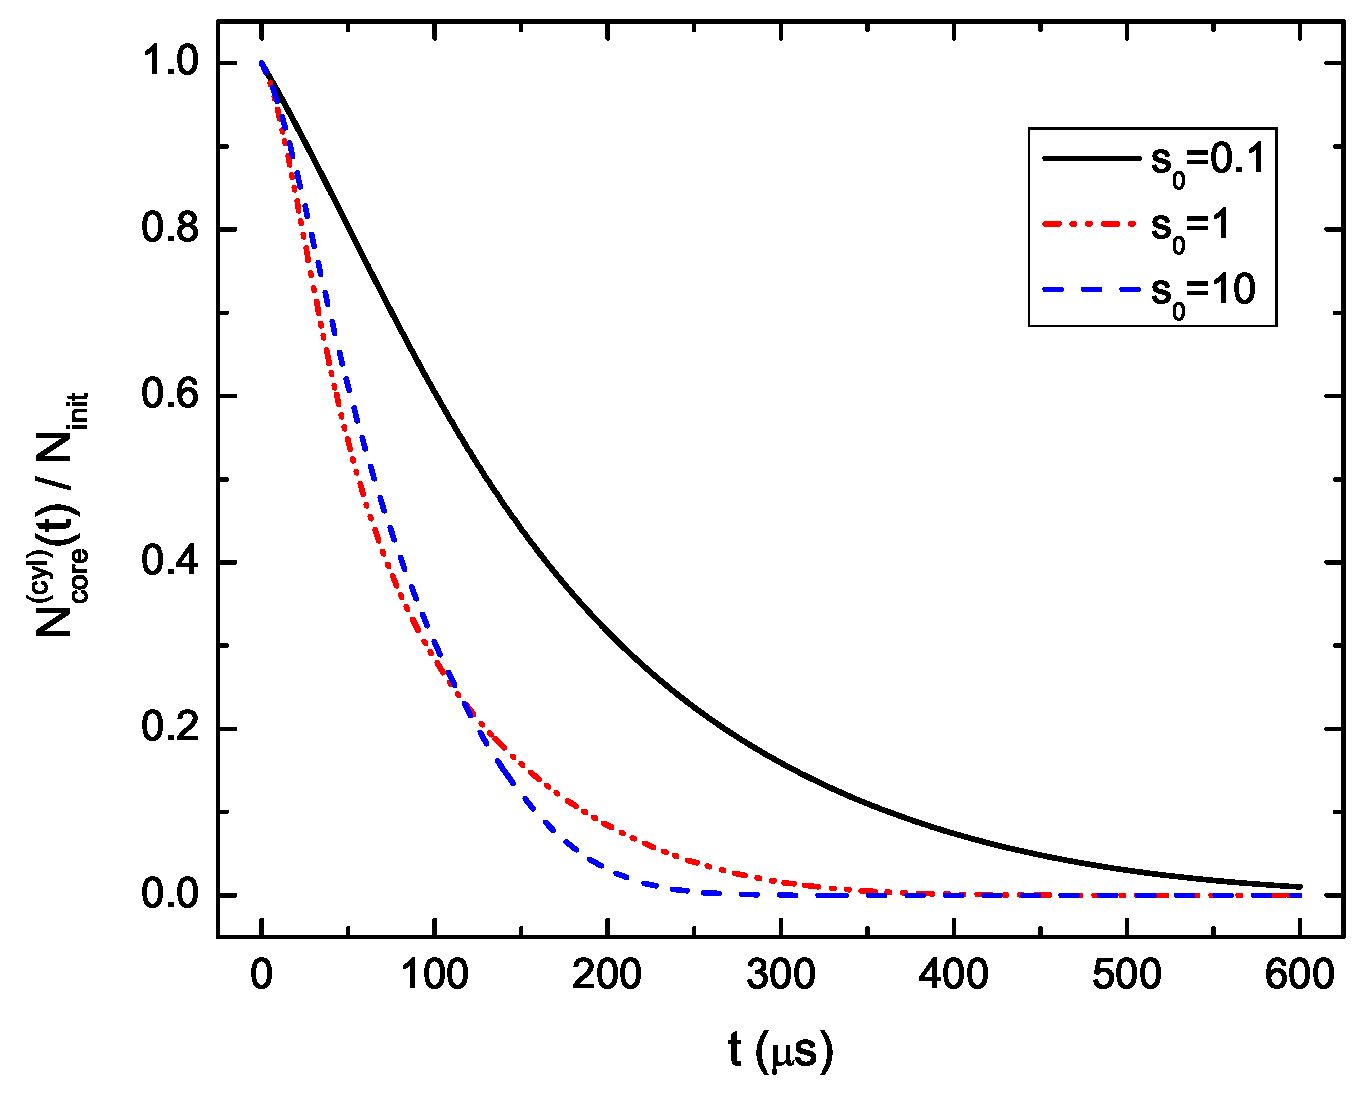
\includegraphics[width=0.7\linewidth]{pics/currmea/Ncyl.eps}
    \caption{A plot of $N_{core}^{(cyl)}(t)$ normalized by its initial value $N_{init}$. Each solid line corresponds to a different $s_0$ parameter of the excitation laser beam. A higher $s_0$ generally means a faster decay in the number of atoms and the pushing effect is more evident. For the smallest $s_0$, the decay is exponential with a time constant $\tau_d$.}
    \label{fig:Ncorecyl}
\end{figure}
This is always a monotonously decreasing function mainly due to the lower density outside the core region. For a very low saturation parameter ($s_0=0.1$) the pushing effect become less important and the dominant loss process of atoms is the diffusion out of the cylinder, which means that the number of atoms decays exponentially with a time constant $\tau_d$.\\

\subsection{Atoms diffusing into the cylinder} 
Apart from the atoms that are present in the cylinder at $t=0$, there is also a contribution of atoms that diffuse into the cylinder. The diffusion flux density into the cylinder is given by
\begin{equation}
	\phi_{diff}^{(in)}(z') = \frac{1}{4} n(z') \langle v \rangle,
  \label{eq:diffin3}
\end{equation}
with $z'$ the coordinate at which a particle enters the cylinder. This flux needs to be integrated over the surface area ($dA_{cyl}=2 \pi \sqrt{2} \sigma_e dz'$) in order to get the inward diffusion flux
\begin{equation}
	\frac{d N_{cyl}}{d t} = \int_{-\infty}^{\sqrt{\frac{\pi}{2}} \sigma_i}{\phi_{diff}^{(in)}(z') 2 \sqrt2 \pi \sigma_e dz'}.
  \label{eq:diffin}
\end{equation}
This rate should be integrated over time to get the number of atoms that have entered the cylinder. However, these atoms can also diffuse out of the cylinder again and only the number of atoms that make it to the core region is interesting for this model.
 
A change of variable $z' = z - d(t')$, where $z$ is the position of a particle which entered the core at a position $z'$ after a time of flight $t'$, is done in order to integrate over the core region instead of over the cylinder,
\begin{equation}
	\frac{d N_{core}^{(diff)}}{d t} = \frac{\pi}{\sqrt2} \sigma_e \langle v \rangle \int_{-\sqrt{\frac{\pi}{2}} \sigma_i}^{\sqrt{\frac{\pi}{2}} \sigma_i} {n(z-d(t)) dz}.
  \label{eq:diffin2}
\end{equation}
Therefore, the contribution of the atoms that diffused into the cylinder to the number of the excited atoms in the core region is given by
\begin{equation}
	N_{core}^{(diff)}(t) \dot{=} \pi^{3/2} \sigma_e \sigma_i \langle v \rangle \int_0^t{n(-d(t')) e^{-\frac{t'}{\tau_d}} f(s_0,\delta) dt'}.
  \label{eq:Ncorediff}
\end{equation}
This expression has also been approximated using the midpoint rule. Note that $N_{core}^{(diff)}(t)$ is the time integral of equation (\ref{eq:Ncorecyl}) apart from some constants.

Figure \ref{fig:Ncorediff} plots $N_{core}^{(diff)}(t)$ for three values of the saturation parameter.
\begin{figure}[tbh!]
    \centering
        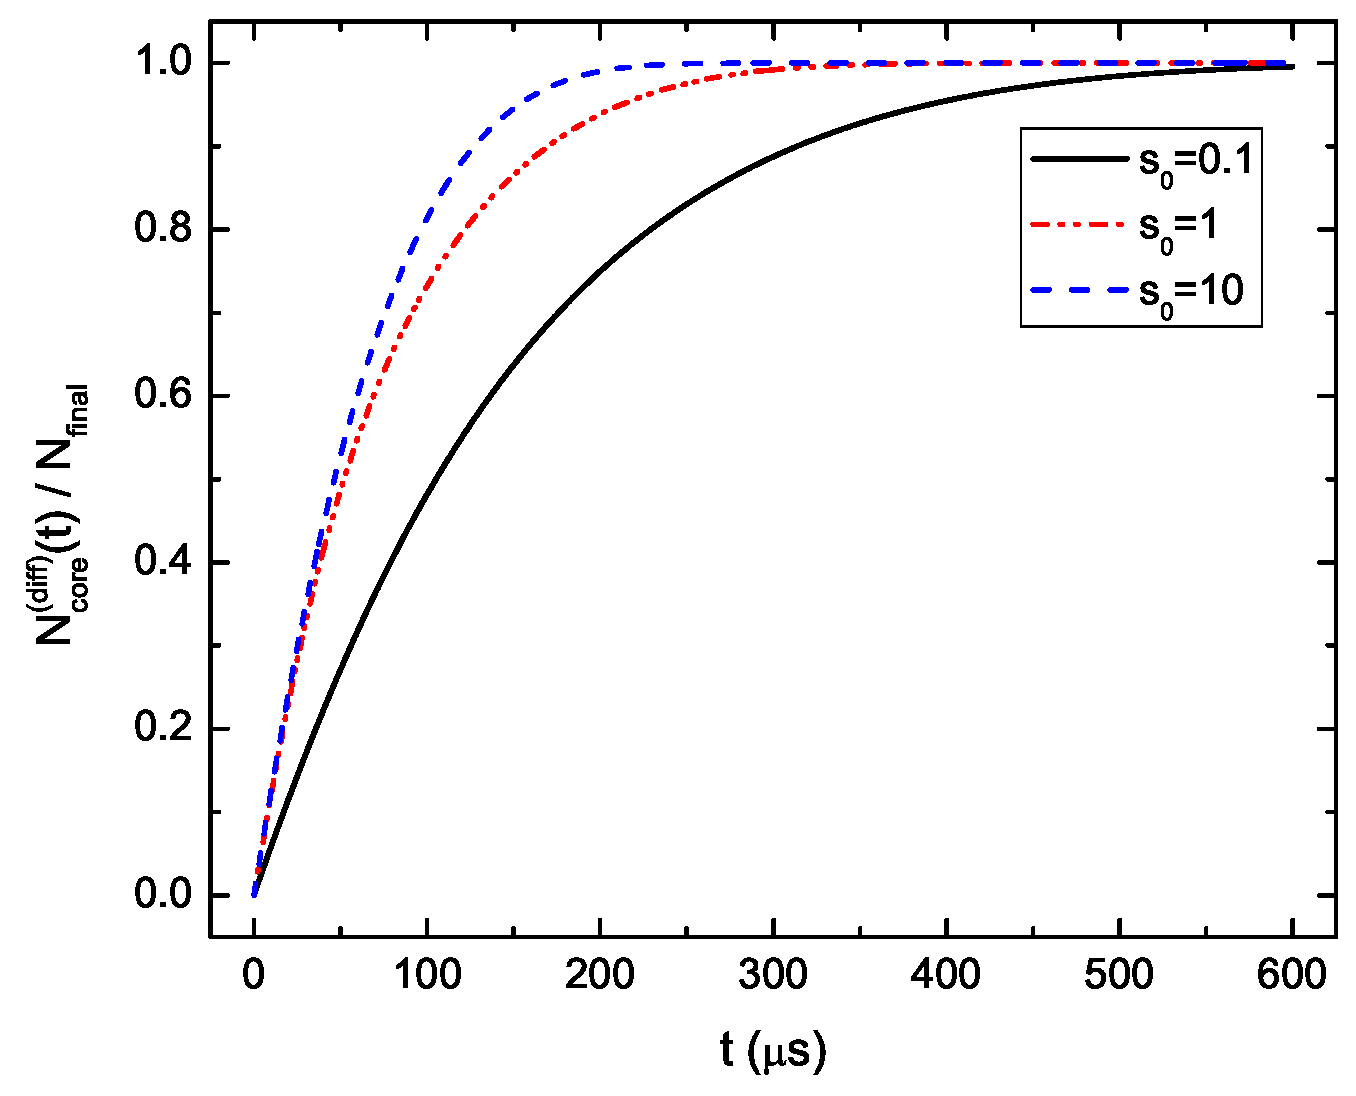
\includegraphics[width=0.7\linewidth]{pics/currmea/Ndiff.eps}
    \caption{A plot of $N_{core}^{(diff)}(t)$ normalized by its initial value $N_{final}$. Each solid line corresponds to a different $s_0$ parameter of the excitation laser beam. A higher $s_0$ generally corresponds to a faster increase in the number of atoms, meaning a stronger ``pushing effect''. For the smallest $s_0$, the increase is exponential with a time constant $\tau_d$.}
    \label{fig:Ncorediff}
\end{figure}
It has been normalized with its maximum value $N_{final} \equiv N_{core}^{(diff)}(\infty)$. This is a monotonously increasing function because at large $t$, the atoms still diffuse into the part of the cylinder close to the core region at the same rate. For a large saturation parameter ($s_0=10$), the convergence to the final value is faster, as for a low saturation parameter the pushing effect is less important.

\subsection{Comparison} Both Figs.\ \ref{fig:Ncorecyl} and \ref{fig:Ncorediff} have been normalized and it is interesting to see how the normalization constants $N_{init}$ and $N_{final}$ relate to each other. This is shown in figure \ref{fig:CompDiffCyl}, where $N_{init}$ and $N_{final}$ are plotted versus $s_0$.
\begin{figure}[tbh!]
    \centering
        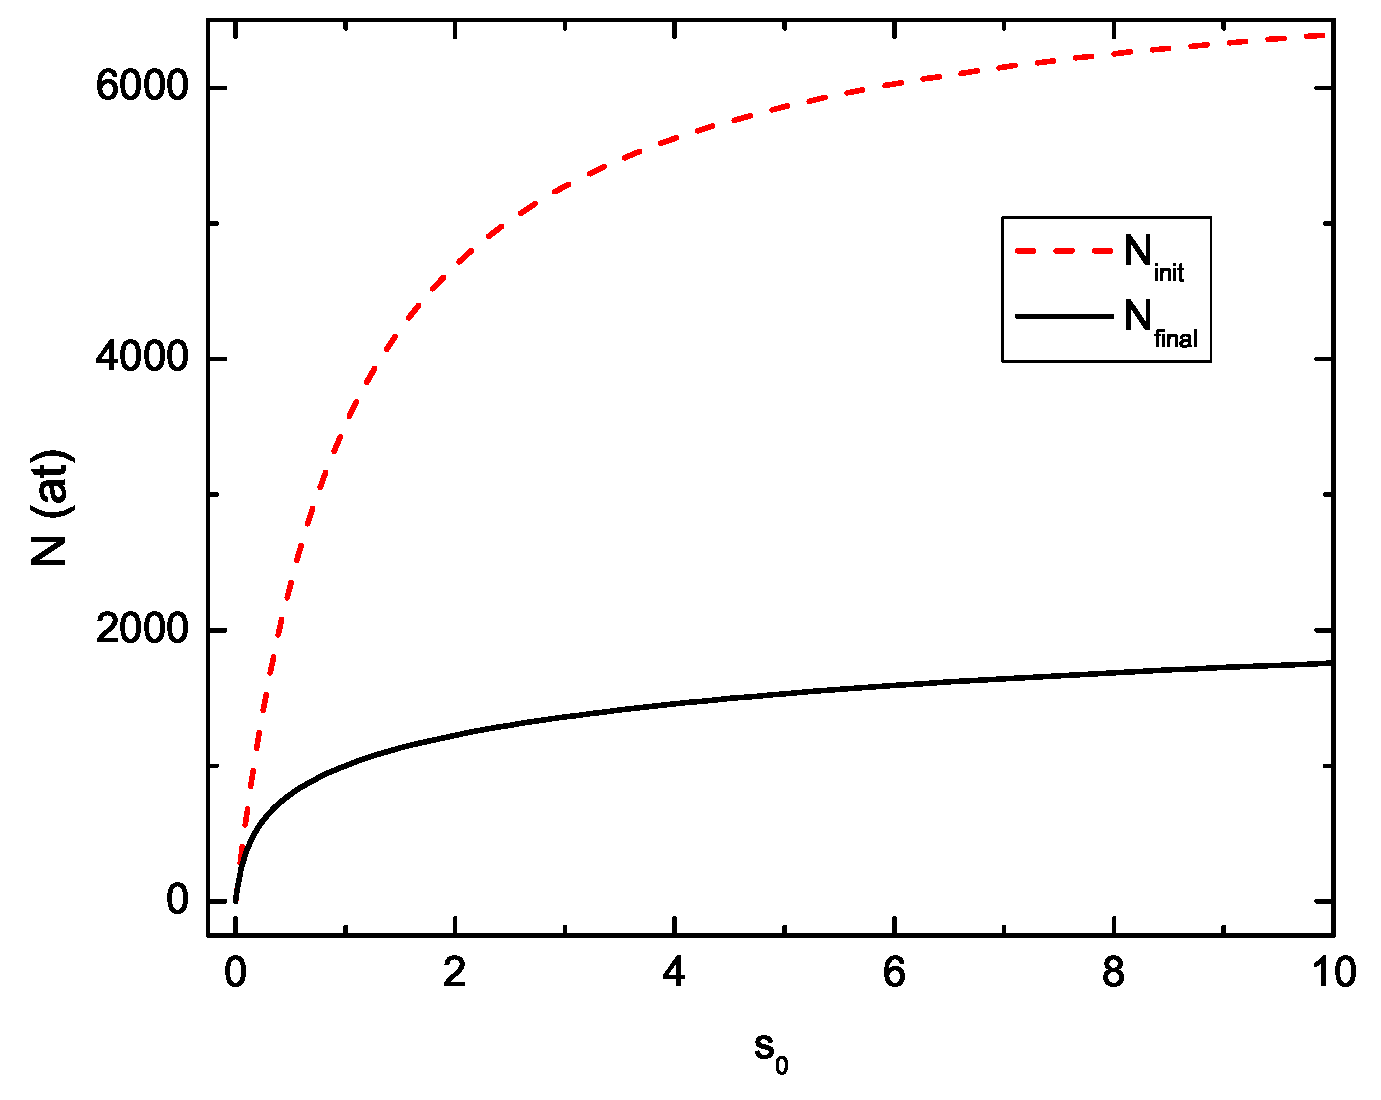
\includegraphics[width=0.7\linewidth]{pics/currmea/Ncyl0AndDiffInf.eps}
    \caption{A plot of $N_{init}$ and $N_{final}$ versus $s_0$. Both are monotonously increasing functions. Hence, a larger saturation parameter is beneficial to the magnitude of both the initial and final currents.}
    \label{fig:CompDiffCyl}
\end{figure}
Both of the functions increase for a larger saturation parameter. Hence, for the current optimization a larger value of the saturation parameter of the excitation laser beam is beneficial. For a finite $s_0$, the following relation holds: $N_{init}>N_{final}$.

\subsection{Extracted current} The ionization rate $r_i$ for excited atoms in the core region can be expressed as
\begin{equation}
    r_i = \tau_i^{-1} = \frac{\sigma_{PI} P_i \lambda_i}{A_i h c},
    \label{eq:r_ion}
\end{equation}
where $\sigma_{PI} = 1.48 \times 10^{-17}$ cm$^2$ is the photo-ionization cross section for $^{85}$Rb \cite{Gabbanini_OC_97}, the ionization laser beam is focused to an area $A_i = 2 \pi \sigma_i^2$, $h$ is Planck's constant and $c$ is the speed of light. The quantity $\tau_i$ is the typical time it takes for an atom to be ionized. 
The available ionization laser beam power in the laboratory is currently such that the average time spent by the atoms in the core region is small compared to the ionization time constant. Therefore, the number of ionized atoms is small (less than 30\%) compared to the total number of atoms present in the core region. 
The time-dependent ion current $I(t)$, in this limit, is given by
\begin{equation}
    I(t) = e r_i \{ N_{core}^{(diff)}(t) + N_{core}^{(cyl)}(t) \}.
    \label{eq:current}
\end{equation}

The typical temporal behavior of the ion current has been plotted in figure \ref{fig:TypicalCurrentProfile}. 
\begin{figure}[tbh!]
    \centering
        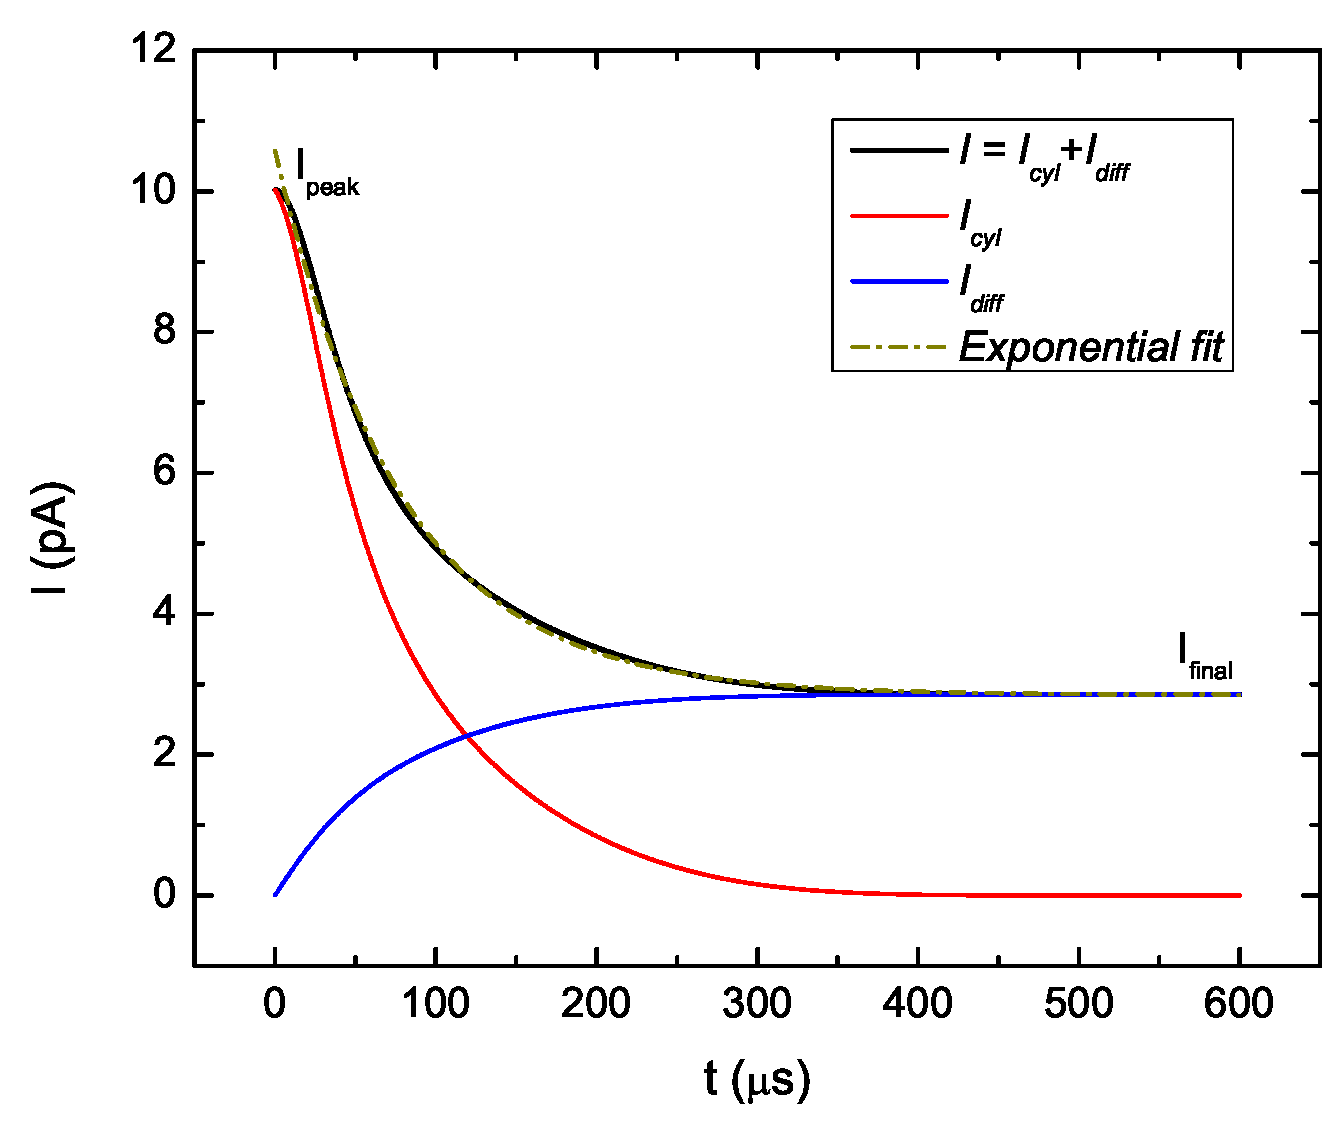
\includegraphics[width=0.7\linewidth]{pics/currmea/TypicalCurrentProfile.eps}
    \caption{A plot of the behavior of the modeled current $I(t)$ and its separate contributions $I_{diff}$ and $I_{cyl}$ as a function of time, at $s_0=1$. An exponential decay is plotted as a dashed line. The maximum current is indicated with $I_{peak}$ and the steady-state current with $I_{final}$.}
    \label{fig:TypicalCurrentProfile}
\end{figure}
In this plot, the current has been separated in these two contributions (similarly as discussed before for the number of atoms in the core region). The diffusion current $I_{diff}(t) = e r_i N_{core}^{(diff)}(t)$ increases with time, up to a final value. In contrast, the current due to atoms starting in the cylinder $I_{cyl}(t) = e r_i N_{cyl}^{(diff)}(t)$ decreases to zero with time. The total current $I(t) = I_{diff}(t) + I_{cyl}(t)$ typically resembles an exponential decay with a time constant $\tau$, with an initial maximum $I_{peak}$ and a steady level $I_{final}$.

It is also useful to define the average current $\overline{I}$, the peak current $I_{peak}$, the final current $I_{final}$ and the charge per pulse $Q$:
\begin{equation}
    \overline{I} = \frac{1}{t_{cycle}} \int_0^{t_i}{I(t)dt},
    \label{eq:avg_current}
\end{equation}
\begin{equation}
    I_{peak} = \mbox{max} \left(I(t)\right),
    \label{eq:peak_current}
\end{equation}
\begin{equation}
    I_{final} = I(t_i),
    \label{eq:final_current}
\end{equation}
\begin{equation}
    Q = \int_0^{t_i}{I(t)dt}.
    \label{eq:charge}
\end{equation}

Figure \ref{fig:TypicalAverageCurrent} shows a typical two-dimensional plot of the average current as a function of the ionization time on the horizontal scale and of the loading time on the vertical scale.
\begin{figure}[tbh!]
    \centering
        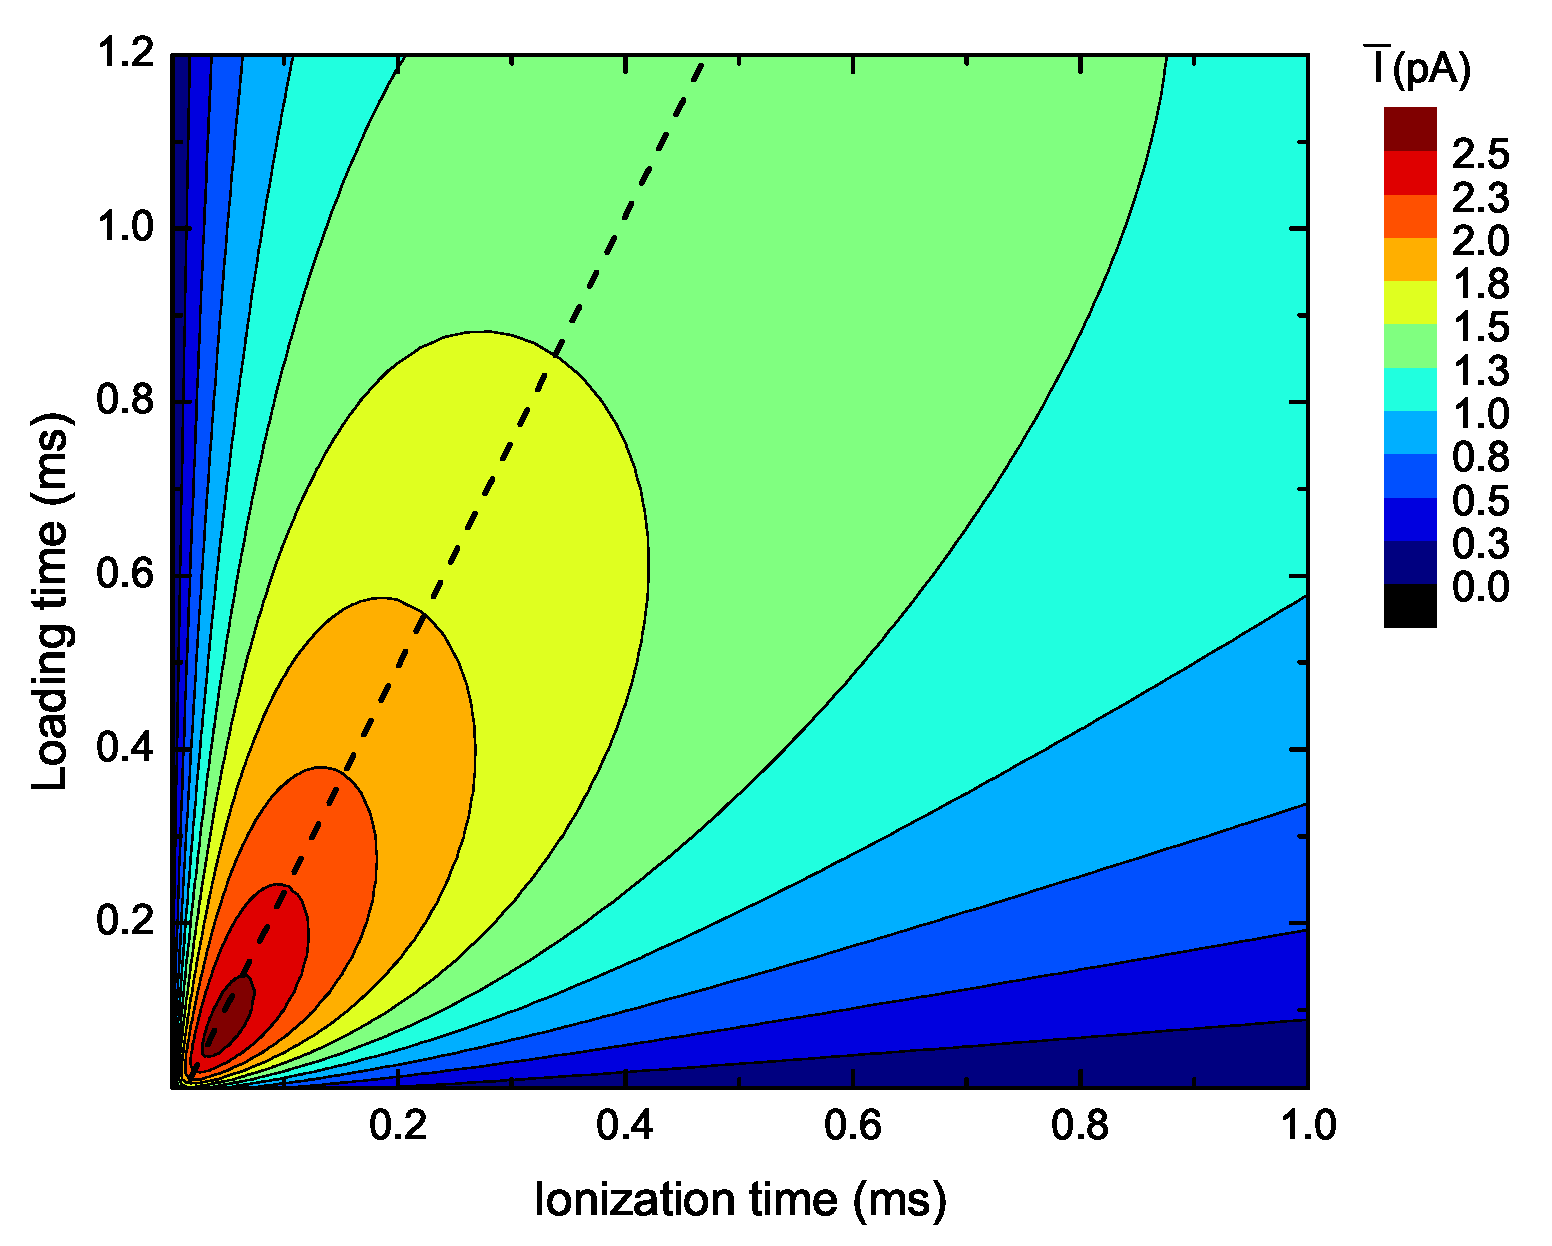
\includegraphics[width=0.7\linewidth]{pics/currmea/TypicalAverageCurrent.eps}
    \caption{Behavior of the modeled average current (color scale) versus the loading time (vertical axis) and the ionization time (horizontal axis), at $s_0=1$. There is a clear optimum for $t_l \approx 100$ $\mu$s and $t_i \approx 50$ $\mu$s. The dashed line highlights the optimal ratio between loading and ionization times for the highest obtainable current.}
    \label{fig:TypicalAverageCurrent}
\end{figure}
A clear maximum is $\overline{I}=2.5$ pA obtained with $t_i \approx 50$ $\mu$s and $t_l \approx 100$ $\mu$s. The loading time is twice the ionization time, corresponding to $\langle N \rangle = N_{\infty}/2$, from equation (\ref{eq:aveN}). From the type of plot shown in figure \ref{fig:TypicalAverageCurrent}, a few important quantities can be extrapolated. The first one is simply the maximum of the average current $\overline{I}_{max}$. Also, for a given ionization time for which the average current is maximized there is an optimum. A curve is drawn as a dashed line in figure \ref{fig:TypicalAverageCurrent} that indicates the dependence. To first order, the curve is a straight line that can be characterized by its slope. We extract the slope by linear regression. The slope $\rho=t_l/t_i$ represents the optimal ratio between the loading and the ionizing times, and is related to the optimal duty cycle $D$ at which the highest current is obtained. The duty cycle is given by
\begin{equation}
    D=\frac{t_i}{t_{cycle}} \cong \frac{1}{\rho + 1},
    \label{eq:Dcycle}
\end{equation}
where the 10 $\mu$s in the definition of $t_{cycle}$ have been ignored since $t_{cycle} \gg 10$ $\mu$s.

\section{Experimental results} \label{sec:expres}
The goal of the measurements is the optimization of the extracted current and the verification of the model described in section \ref{sec:model}. In order to achieve these objectives, first the parameters of the model have been experimentally determined: the temperature $T_s$ of the trapped atoms, the loading rate of the MOT $R_L$ and the lifetime of the MOT with trapping laser beams turned on ($\tau_M$) and while they are turned off ($\tau'_M$). Table \ref{tab:measPar} summarizes the measured parameters for the model presented in section \ref{sec:model}.
\begin{table}[ht]
	\caption{\label{tab:measPar} Measured parameters of the model.}
	\begin{center}
		\begin{tabular}{| l | l | l |  }
			\hline
			Parameter & Symbol & Value \\ \hline
			Source temperature & $T_s$ & $(230 \pm 30)$ $\mu$K \\
			Loading rate & $R_L$ & $(12 \pm 1) \times 10^8$ s$^{-1}$ \\ 
			MOT Lifetime (trap on) & $\tau_M$ & $(180 \pm 5)$ ms \\ 
			MOT Lifetime (trap off) & $\tau'_M$ & $(71 \pm 6)$ ms \\
			\hline
		\end{tabular}
	\end{center}
\end{table}

\subsection{Parameters of the model}
\label{sec:param}
{\bf Trap temperature.} The trap temperature is an important parameter in our model, as it affects the diffusion between the core region and the rest of the MOT, as well for the expansion of the MOT itself while the trapping lasers are turned off. After the trapping laser beams are turned off at $t=0$, the MOT expands according to the relation
\begin{equation}
    \sigma_M^2(t_e) = \sigma_M^2(0) + \left(\frac{k_b T_s}{m}\right) t_e^2,
    \label{eq:sigma_MOT}
\end{equation}
where $k_b$ is Boltzmann's constant \cite{Weiss_JB_89}. 
The MOT cameras are triggered to measure the fluorescence light emitted by the trapped atoms at a variable delay time up to 8~ms after the trapping lasers are turned off (at $t=0$). The trapping laser beams are flashed on for 250 $\mu$s to produce the fluorescence light. The \textit{rms}-radii of the MOT are calculated by fitting the images with a 2D-Gaussian. The square of the \textit{rms}-radius of the MOT is plotted versus the square of the expansion time in figure \ref{m1}.
\begin{figure*}[tbh!]
	\subfloat[Source temperature\label{m1}]{\includegraphics[width=0.48\linewidth]{pics/currmea/Temperature}}
	\hfill	
	\subfloat[Loading rate\label{m2}]{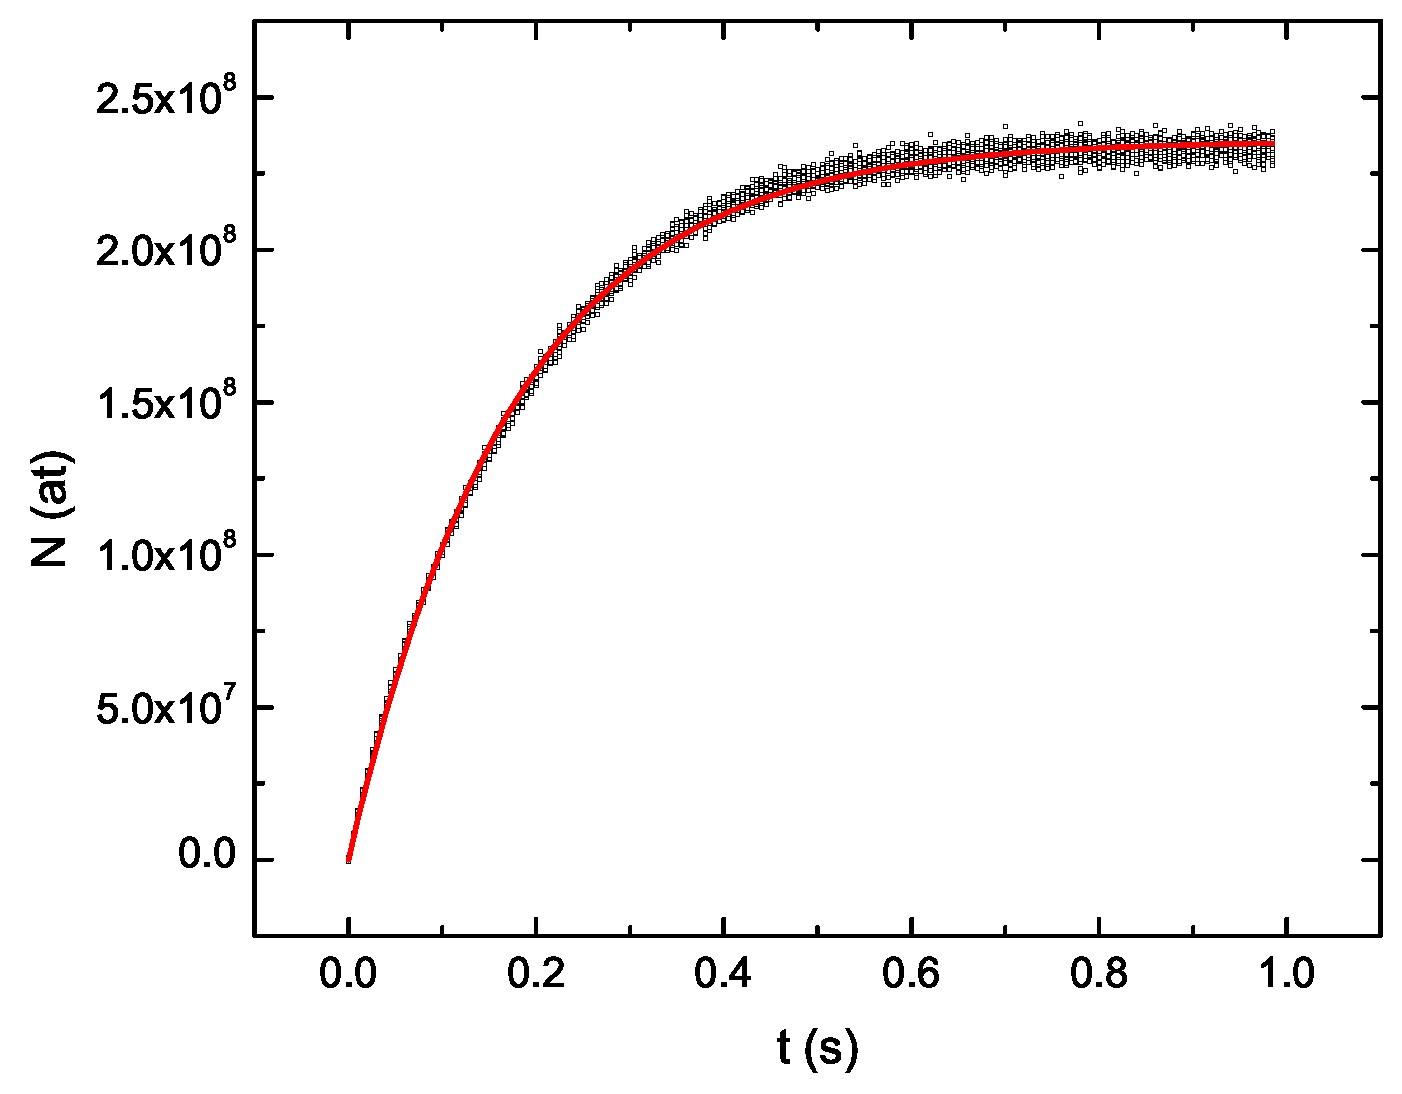
\includegraphics[width=0.48\linewidth]{pics/currmea/LoadingRate}}
	\\
	\subfloat[Number of atoms\label{m3}]{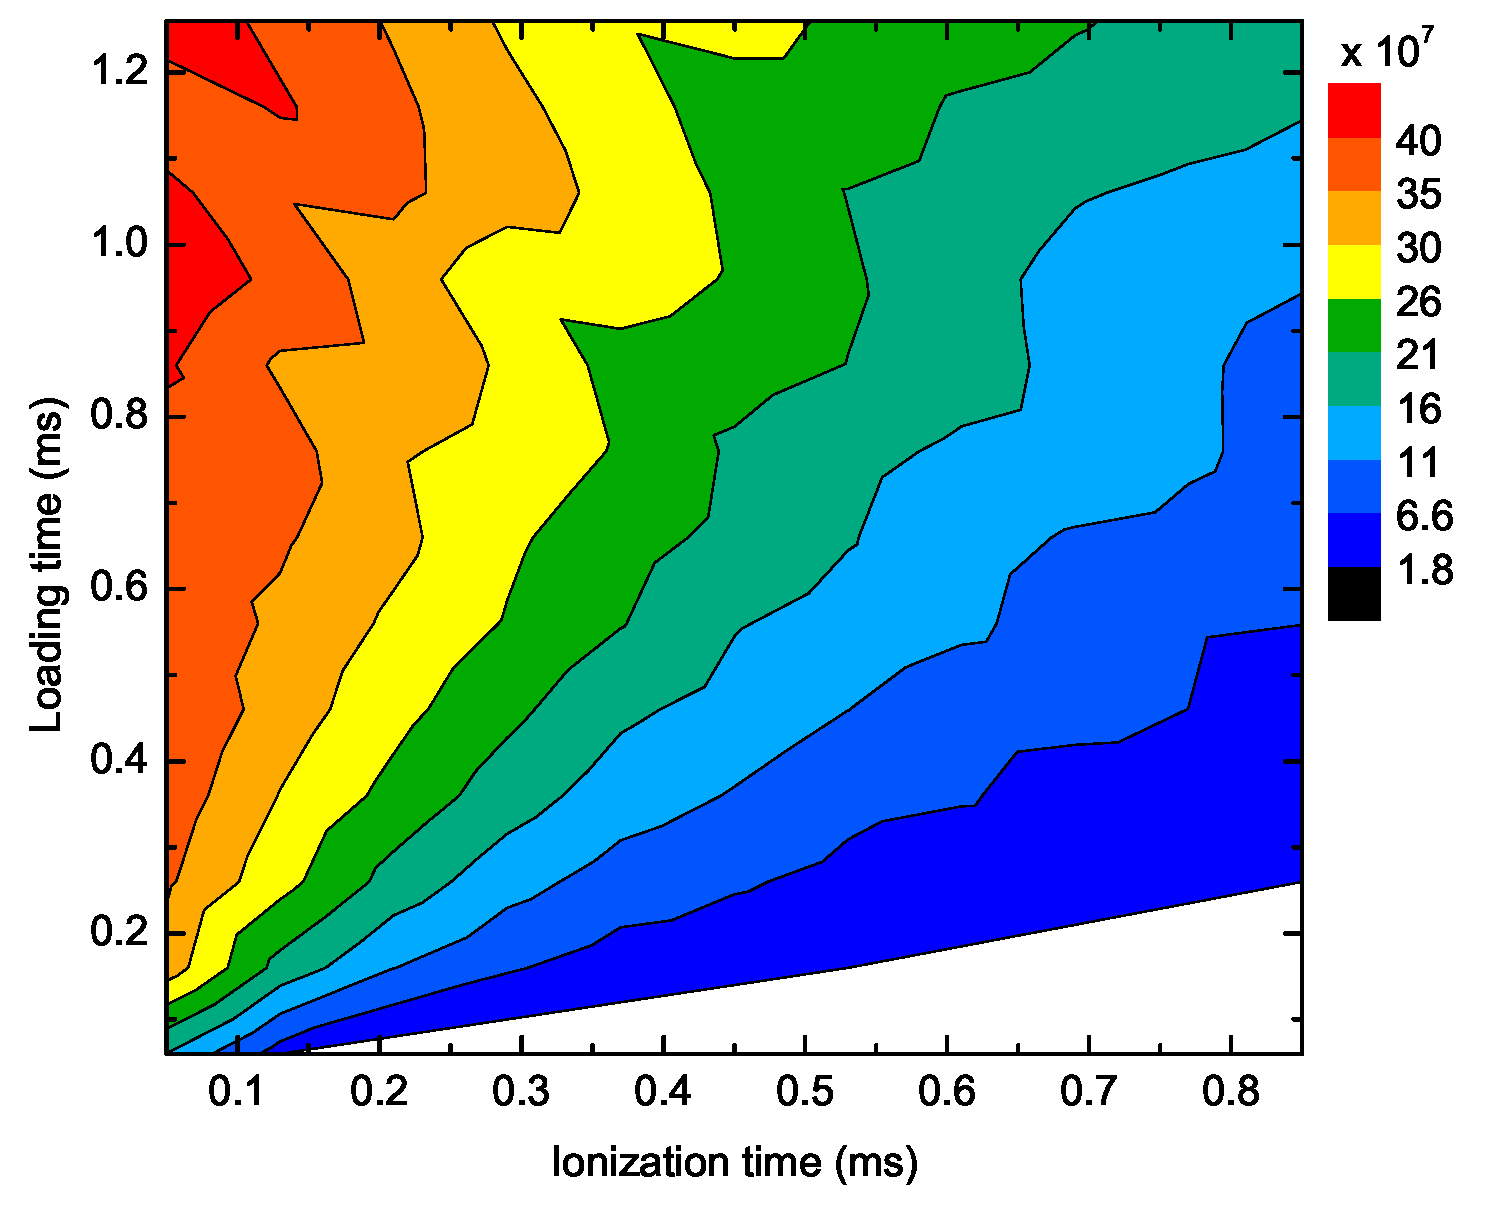
\includegraphics[width=0.48\linewidth]{pics/currmea/NumberAtoms2DPlot}}
	\hfill	
	\subfloat[Number of atoms\label{m4}]{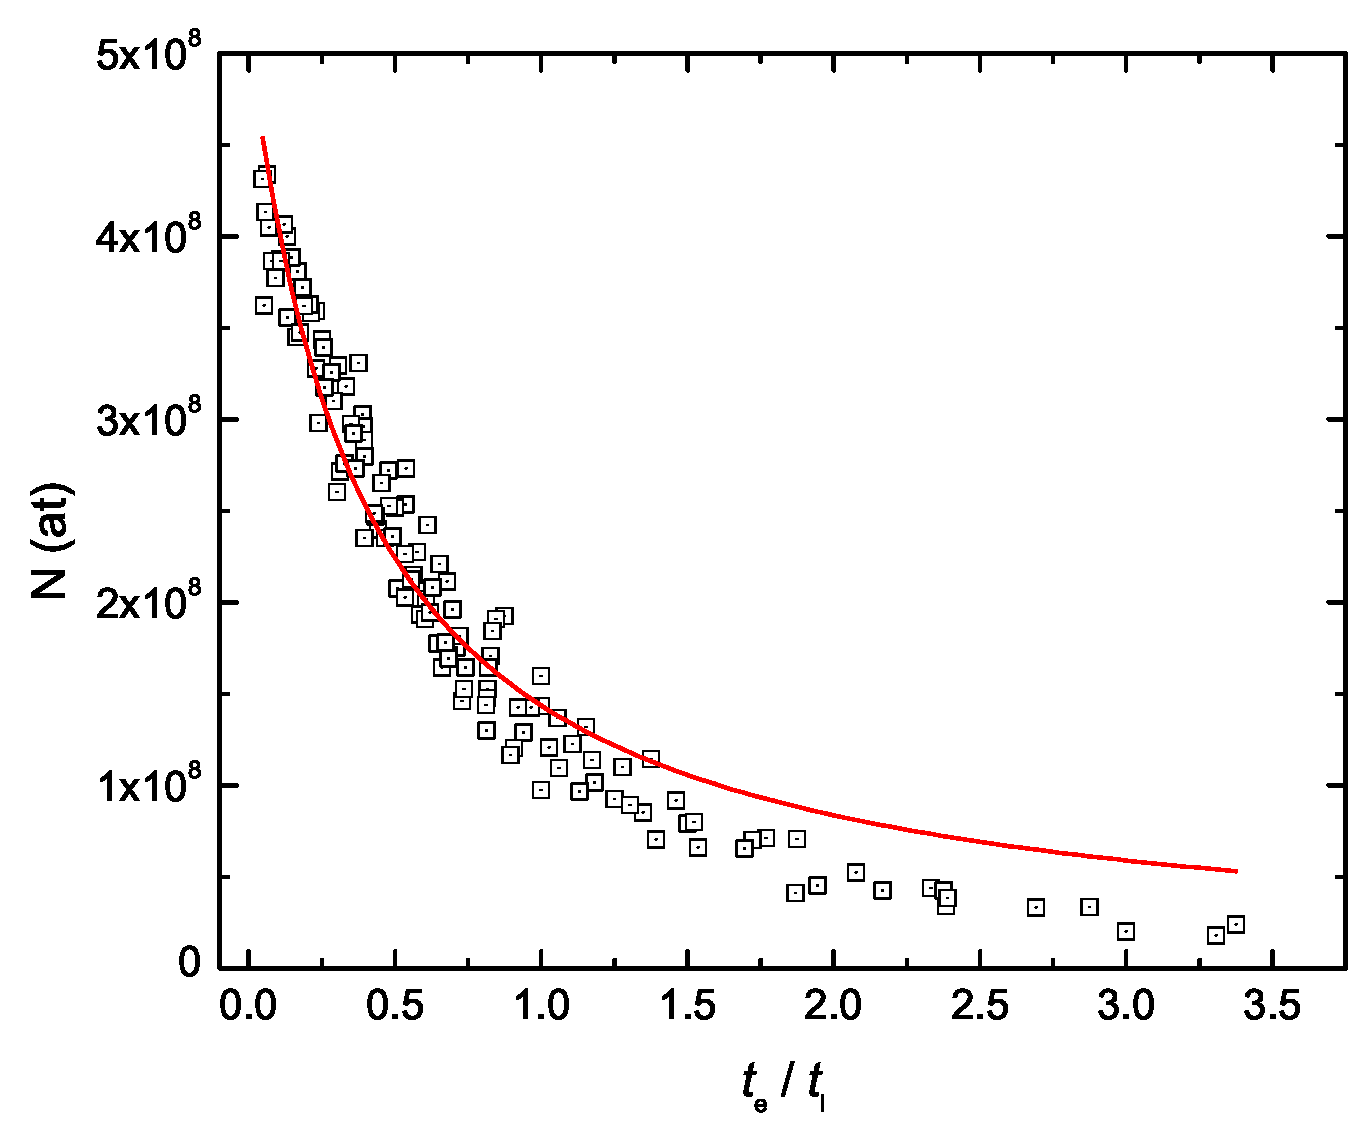
\includegraphics[width=0.48\linewidth]{pics/currmea/NumberAtomsCombinedXaxis}}	
	\caption{In panel (a), a typical result of the source temperature measurements is shown. The square of the \textit{rms}-radii of the MOT are plotted versus the expansion time squared. In panel (b), the number of atoms in the MOT while loading the MOT is plotted versus the time. The data is fitted with equation (\ref{eq:RL_rate}) in order to determine the loading rate of the MOT and its lifetime. In panel (c), a contour plot of the number of atoms versus the ionization time and the loading time is shown. In panel (d), a plot of the number of atoms in the MOT versus the ratio of the expansion and the loading times is shown. The data is fitted with equation (\ref{eq:aveN}) in order to determine the lifetime with trapping laser beams off. \label{fig:parameas}}
\end{figure*}
The trap temperature, determined from a fit of equation (\ref{eq:sigma_MOT}) to the data, is $(230 \pm 30)~\mu$K, not far from the Doppler temperature $T_D = 143$ $\mu$K of the $^{85}$Rb transition. The uncertainty in the extracted temperature reflects the degree of agreement between data sets.\\

\noindent {\bf Loading rate and lifetime.} Starting with an empty trap, at $t=0$ the trapping laser beams are turned on and the amount of fluorescent light emitted by the trapped atoms is monitored with two calibrated CCD cameras. The exposure time of the cameras is 5 ms and they are triggered at intervals of 40 ms and different measurement sweeps were shifted in steps of 5 ms. The measurement is repeated 25 times for sufficient statistical accuracy. The pixel counts of one camera image are then summed and the number of atoms is calculated. Figure \ref{m2} shows a typical result of the experiment. The result is fitted with equation (\ref{eq:RL_rate}), giving $\tau_M = (180 \pm 5)$~ms and $R_L = (12 \pm 1) \times 10^8$~atoms/s. The 10~\% accuracy reflects the degree of agreement between the two cameras.\\

\noindent {\bf Number of Atoms.} The average number of trapped atoms $\langle N \rangle$ under continuous cycling was determined with the CCD cameras for a range of loading and ionization times. The measured number of atoms is plotted versus the ionization time and the loading time in figure \ref{m3}. The contour lines are in first approximation straight lines passing through the origin. Therefore the number of trapped atoms is a function of the combined variable $t_e/t_l$ and a plot is shown in figure \ref{m4}. The solid line is a fit according to equation (\ref{eq:aveN}). The fit follows the overall trend but it is too high for large $t_e/t_l$. However this deviation is not important since the optimum for the current occurs at $t_e/t_l < 1$, where there is a good agreement. Finally, the last missing parameter of the model can be calculated. From the fit, it follows $\zeta = 2.5 \pm 0.1$ and $\tau'_M = (71 \pm 6)$ ms, using the measured value of $\tau_M = (180 \pm 5)$ ms measured previously in this section.\\

\subsection{Typical current signal}
\label{sec:typcurrent}
This section discusses the temporal behavior of the measured current pulses. Two measurements have been selected and are shown in figure \ref{fig:signals}: the first for a large saturation parameter $s_0=4$ and $t_i=130$ $\mu$s, and the second one for a smaller saturation parameter $s_0=0.2$ and $t_i=770$ $\mu$s. The loading time is $t_l=250$ $\mu$s in both cases.
\begin{figure*}[tbh!]
	\subfloat[$s_0 = 4$\label{c1}]{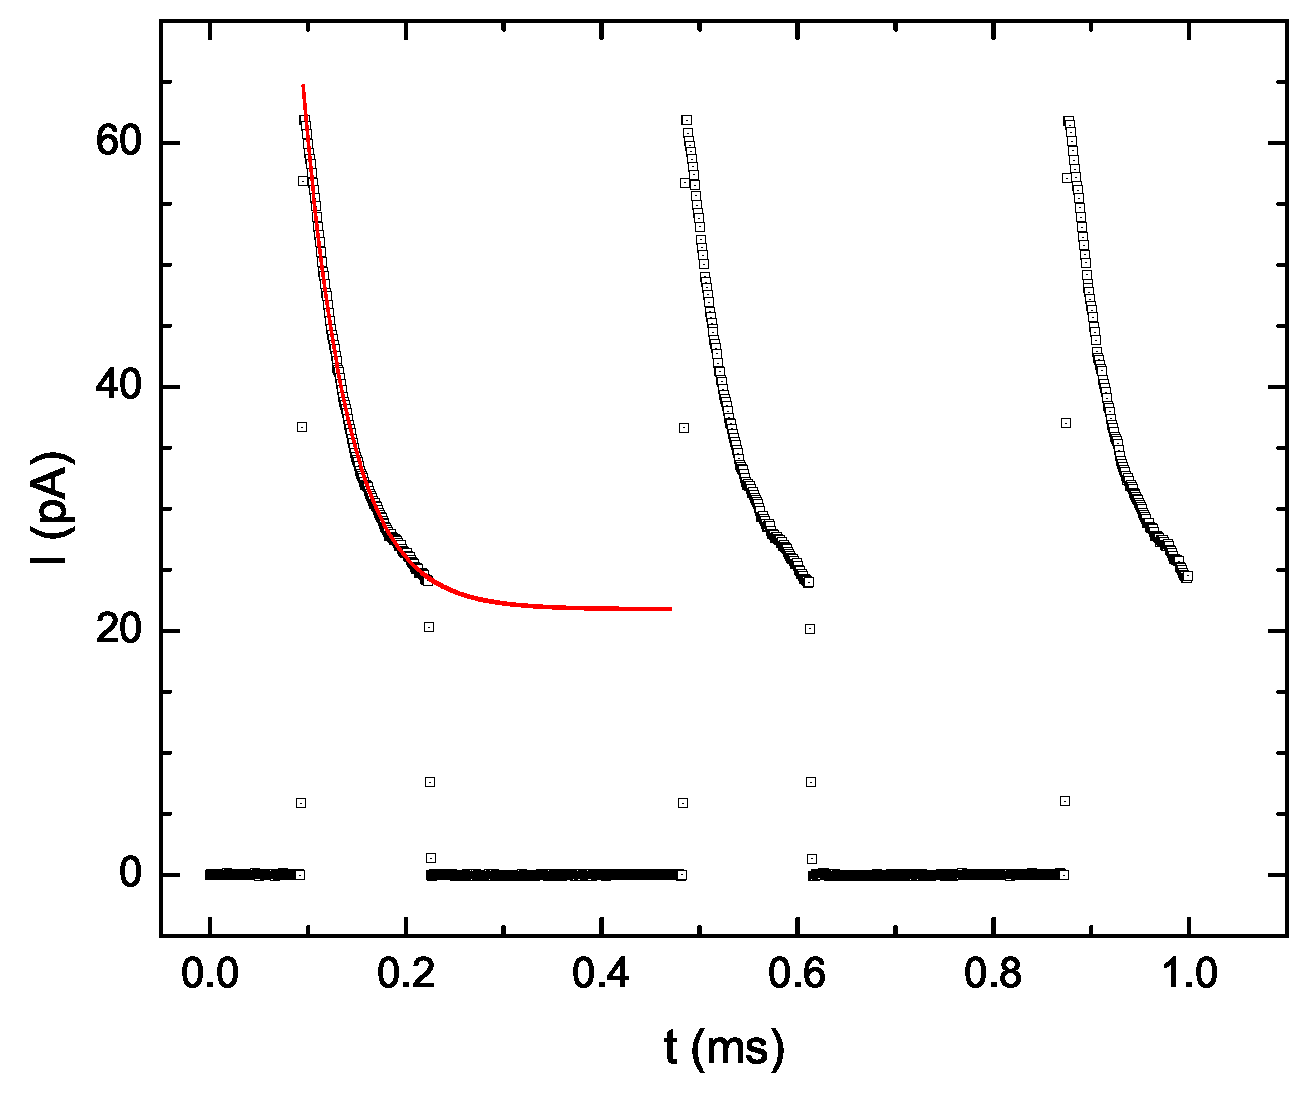
\includegraphics[width=0.48\linewidth]{pics/currmea/CurrentVsTimeS=4}}
	\hfill	
	\subfloat[$s_0 = 0.2$\label{c2}]{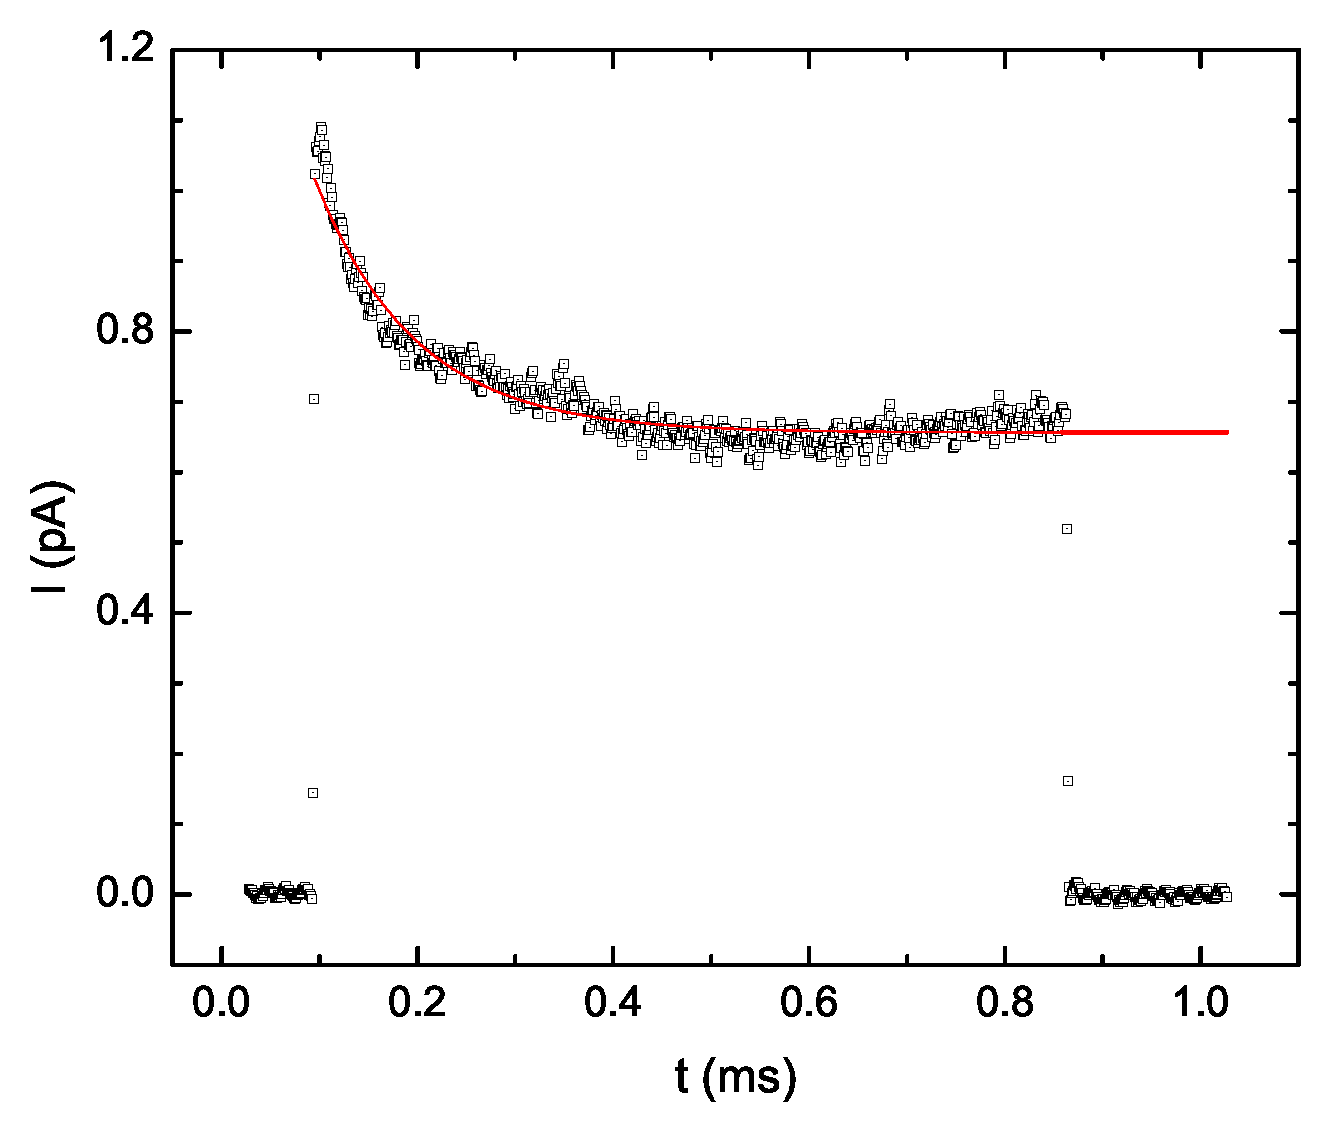
\includegraphics[width=0.48\linewidth]{pics/currmea/CurrentVsTimeS=0,2}}
	\caption{Current plotted versus time for two values of the saturation parameter of the excitation laser beam. The solid line is an exponential fit of the data. The peak current is much larger for $s_0=4$ as well as the ratio $I_{peak}/I_{final}$.\label{fig:signals}}
\end{figure*}
The two plots show a number of differences. One of these is the magnitude of the peak current: $I_{peak}=62$ pA in figure \ref{c1} against $I_{peak}=1.1$ pA in figure \ref{c2}. This is partly caused by the difference in excited state fraction ratio $f(4,0)/f(0.2,0) = 4.8$, but the difference in the number of trapped atoms is more important. In figure \ref{c2}, the ionization time is about 3 times longer than the loading time, while in figure \ref{c1} this is a factor of 2 shorter. From figure \ref{m4}, this corresponds to $\langle N \rangle= 2.5 \times 10^8$ atoms and $2.5 \times 10^7$ atoms respectively. The two effects combined change the peak current by a factor 48, which is comparable with the difference in the peak current in the two measurements (a factor $\approx$~56).

The second difference is the ratio between the peak and the final current $I_{peak}/I_{final}$. This ratio is 2.8 for $s_0=4$ since the final current is $I_{final}=22$ and 1.4 for $s_0=0.2$ since $I_{final}=0.7$ pA. This difference can be explained with the model and it is caused by the different $s_0$ as shown in figure \ref{fig:CompDiffCyl}, where ratios of 3.9 and 2.2 are respective calculated at the same $s_0$. The measured values are both a factor 1.5 lower, possibly due to local variation of the MOT density.

Finally, the currents resemble quite well an exponential decay, with time constants of $\tau = 45$ $\mu$s in figure \ref{c1} and $\tau = 102$ $\mu$s in figure \ref{c2}, drawn as solid lines. The value for figure \ref{c1} is somewhat uncertain because the final current level is not reached yet due to the short $t_i$. Nevertheless, the time constant clearly depends on $s_0$ as predicted by the model (see figures \ref{fig:Ncorecyl} and \ref{fig:Ncorediff}).

\subsection{Moving the ionization laser beam}
\label{sec:verify}
The model predicts that the atoms that are ionized have been pushed into the core region by the excitation laser beam. Therefore the total charge created can be increased by moving the ionization laser beam away from the center of the MOT, in the positive $z$-direction (see figure \ref{fig:setup}). In this way the excitation laser cylinder (see figure \ref{fig:cylGeo}) can be made longer, increasing the number of atoms it contains. However, for larger displacements the current will be reduced once outward diffusion becomes important. In addition, the initial current will be reduced because the ionization laser beam is no longer in the center of the MOT (where the density is maximum). In order to verify this picture, an experiment is performed where the current is measured for several $z$-positions of the ionization laser beam. This experiment uses a long ionization time $t_i = 900$ $\mu$s, so that the current will nearly reach its final value, a very long loading time of $t_l = 5$ ms and $s_0=4$. Here $\Delta z > 0$ corresponds to a displacement of the ionization laser spot in the same direction as the atoms are pushed.
 
For several values of $\Delta z$ (in units of $\sigma_M \approx 0.8$ mm), calculated and measured current profiles have been plotted in figure \ref{fig:dispIoniz}. 
\begin{figure*}[tbh!]
\subfloat[model\label{d1}]{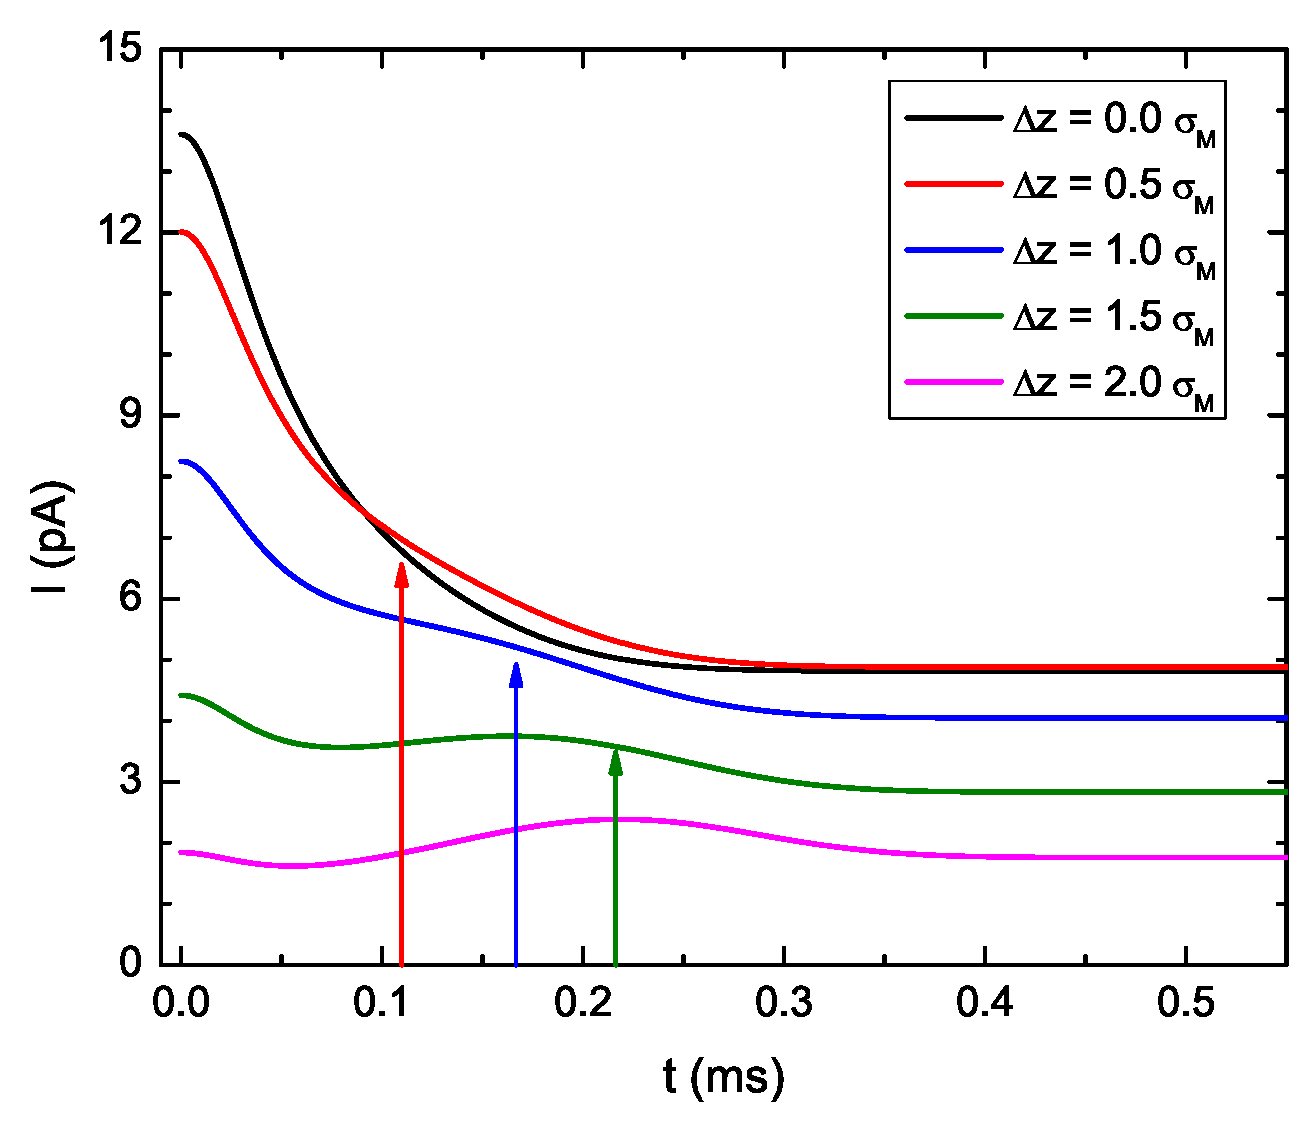
\includegraphics[width=0.48\linewidth]{pics/currmea/IonisationPositionModeledCurrent}}
	\hfill		
	\subfloat[measurement\label{d2}]{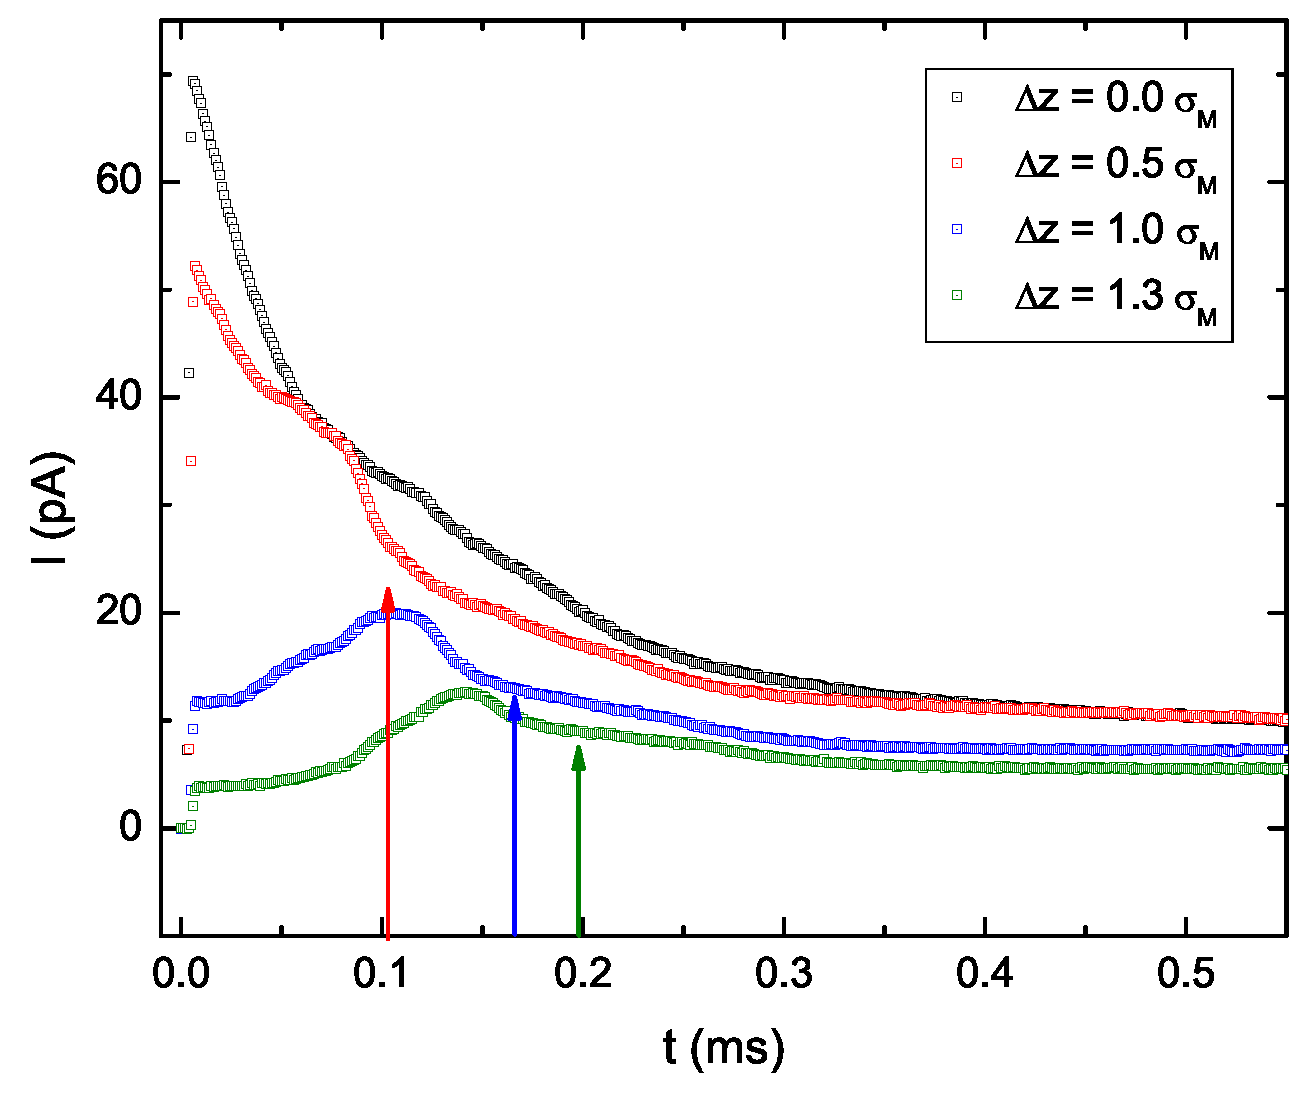
\includegraphics[width=0.48\linewidth]{pics/currmea/IonisationPositionMeasuredCurrent}}
	\caption{Current behavior if the ionization laser is shifted relative to the position where the initial current is maximal at the center of the MOT ($\Delta z = 0$). The figures compare the model predictions and the experimental results for several displacements $\Delta z$. The decay of the current is slower for larger shifts, and a ``bump'' appears on top of the ``exponential decay''. A colored arrow indicates the time when the ``bump'' occurs according to the simple approximation (see text).\label{fig:dispIoniz}}
\end{figure*}
For the calculations, a shifted density term 
\begin{equation}
    n(z)=n_c e^{\left( -(z-\Delta z)^2 / {2 \sigma_M^2} \right)},
    \label{eq:shiftn}
\end{equation}
is used instead of the density at $z=0$ of equation (\ref{eq:density}). Comparing the two figures, a number of similarities are observed. In both cases, the initial current decreases when $\Delta z$ is increased, because the density at the ionization laser position decreases. Also, in both cases, the current gets an extra "bump": it no longer matches an exponential decay, but has a broad peak added to it. The time at which this peak occurs increases with $\Delta z$. It is approximately given by the time needed for an atom to be pushed over the distance $\Delta z$, the solution of equation (\ref{eq:distance}). This gives $t_{peak} = 111$ $\mu$s for $\Delta z= 0.5~\sigma_M$, $t_{peak} = 168$ $\mu$s for $\Delta z = \sigma_M$ and $t_{peak} = 215$ $\mu$s for $\Delta z = 1.5~\sigma_M$, for the model. The first three peak positions based on this approach have been marked with coloured arrows in figure \ref{fig:dispIoniz}. This simple approach does not take into account effects like outward diffusion and increasing of the Doppler shifts, which both will make the real peak occur earlier. Also, because these peaks are superimposed on the exponential decay, the actual peak positions will seem to occur earlier. Nevertheless, it gives quite a good approximation of the behavior in both the model and the experiment.
 
Next, both the model and the experiment show that shifting the ionization laser too far, will result in a lower current for the whole time the ionization laser beam is turned on, compared to $\Delta z =0$. This is the case for $\Delta z \geq \sigma_M$ both in the modeled current and in the experiment. Clearly, the outward diffusion and decreasing excited state fraction for larger time of flight, prevent the extra atoms in the cylinder from being ionized. For smaller shifts, $\Delta z = 0.5~\sigma_M$, both the model and the experiment show a slightly larger final current, which can be desirable for extremely long pulses, where only the final level of the current is relevant. For shifts $0 < \Delta z < 0.5~\sigma_M$ an optimum occurs, where also for shorter ionization times the obtained current is larger than without the shift.

One aspect where the model and experiment do not agree, is how much the initial current decreases when $\Delta z$ is increased. This is probably caused by deviations of the number density from strict Gaussian behavior, observable as asymmetries present in the shape of the MOT. 

\subsection{Current optimization measurement}
\label{sec:currentmea}
The main parameters of the model have been measured in section \ref{sec:param} and the model has been verified in section \ref{sec:verify}. The main goal of this paper is to optimize the extracted current. The average current, equation (\ref{eq:avg_current}), is measured while the loading and the ionization times are varied. This results in a contour plot similar to the one presented in figure \ref{fig:TypicalAverageCurrent}. These measurements have been performed at different values of the excitation laser beam saturation parameter and ionization laser beam power. Every set of measurements is performed in a random order to prevent drift from influencing the results. The measurement time varies between 30 and 60 minutes depending on the number of steps. Typically, the ionization power energy is $P_i=46$~mW, unless specified.\\

\noindent {\bf Saturation parameter dependence.} The saturation parameter is changed by varying the power of the excitation laser beam with the use of an AOM. Figure \ref{fig:smallVdiffs} shows two scans performed at $s_0 = 1$ and $s_0=12$. In both of the scans, $t_l$ is incremented in steps of 100 $\mu$s between 50 and 1250 $\mu$s and $t_i$ ranges between 50 and 850 $\mu$s in steps of 80 $\mu$s, a total of 143 points. 
\begin{figure*}[tbh!]
	\subfloat[$s_0 = 1$\label{s1}]{\includegraphics[width=0.52\linewidth]{pics/currmea/2DPlotS=1}}
	\hfill	
	\subfloat[$s_0 = 12$\label{s2}]{\includegraphics[width=0.45\linewidth]{pics/currmea/2DPlotS=12}}
	\caption{Contour plots of the average current versus the loading time (vertical axes) and the ionization time (horizontal axis), for $s_0=1$ and $s_0=12$. The color scale is the same for both of the plots. The dashed line highlights the slope $\rho$ at which the highest average current occurs. A black dot marks the maximum of the average current. The average current is larger for a higher $s_0$ and the same conclusion is valid for the slope.\label{fig:smallVdiffs}}
\end{figure*}
These plots strongly resemble the one from the model shown in figure \ref{fig:TypicalAverageCurrent}, especially the one at $s_0=12$. In general, a higher saturation parameter is beneficial for increasing the average current. The maximum average current is marked with a black dot in the plots. The average current is about a factor of two higher, $\overline{I} \approx 8.2$~pA at $s_0=12$ compare to $\overline{I} \approx 3.8$ pA at $s_0=1$, and this is mainly caused by the higher excited state fraction: $f(12,0)/f(1,0) \approx 1.8$. A stronger ``pushing effect'' is also important, since it leaves less time for the atoms to diffuse out of the cylinder.\\

It follows from the plot that it is better to ionize for a short time, going for a higher repetition rate rather than a low one. The optimum ratio $\rho$ where the maximum of the average current occurs is drawn as a dashed line in the two figures: $\rho= 2.3$ for $s_0=12$ and $\rho = 1.4$ for $s_0=1$. Clearly it becomes beneficial to use a shorter ionization phase for a higher saturation parameter and this is a direct consequence of the larger ratio between the peak and the final current already discussed in Subsection \ref{sec:typcurrent}.
The maximum average current measured in all the experiments is $(13 \pm 1)$ pA, obtained at a duty cycle of 36\%. The maximum peak current measured is $(88 \pm 5)$ pA. The uncertainty of the current is related to the calibration of the MCP.

The contour plot of the charge per pulse for $s_0=12$ is plotted in figure \ref{fig:charge2Dplot}.
\begin{figure}[tbh!]
    \centering
        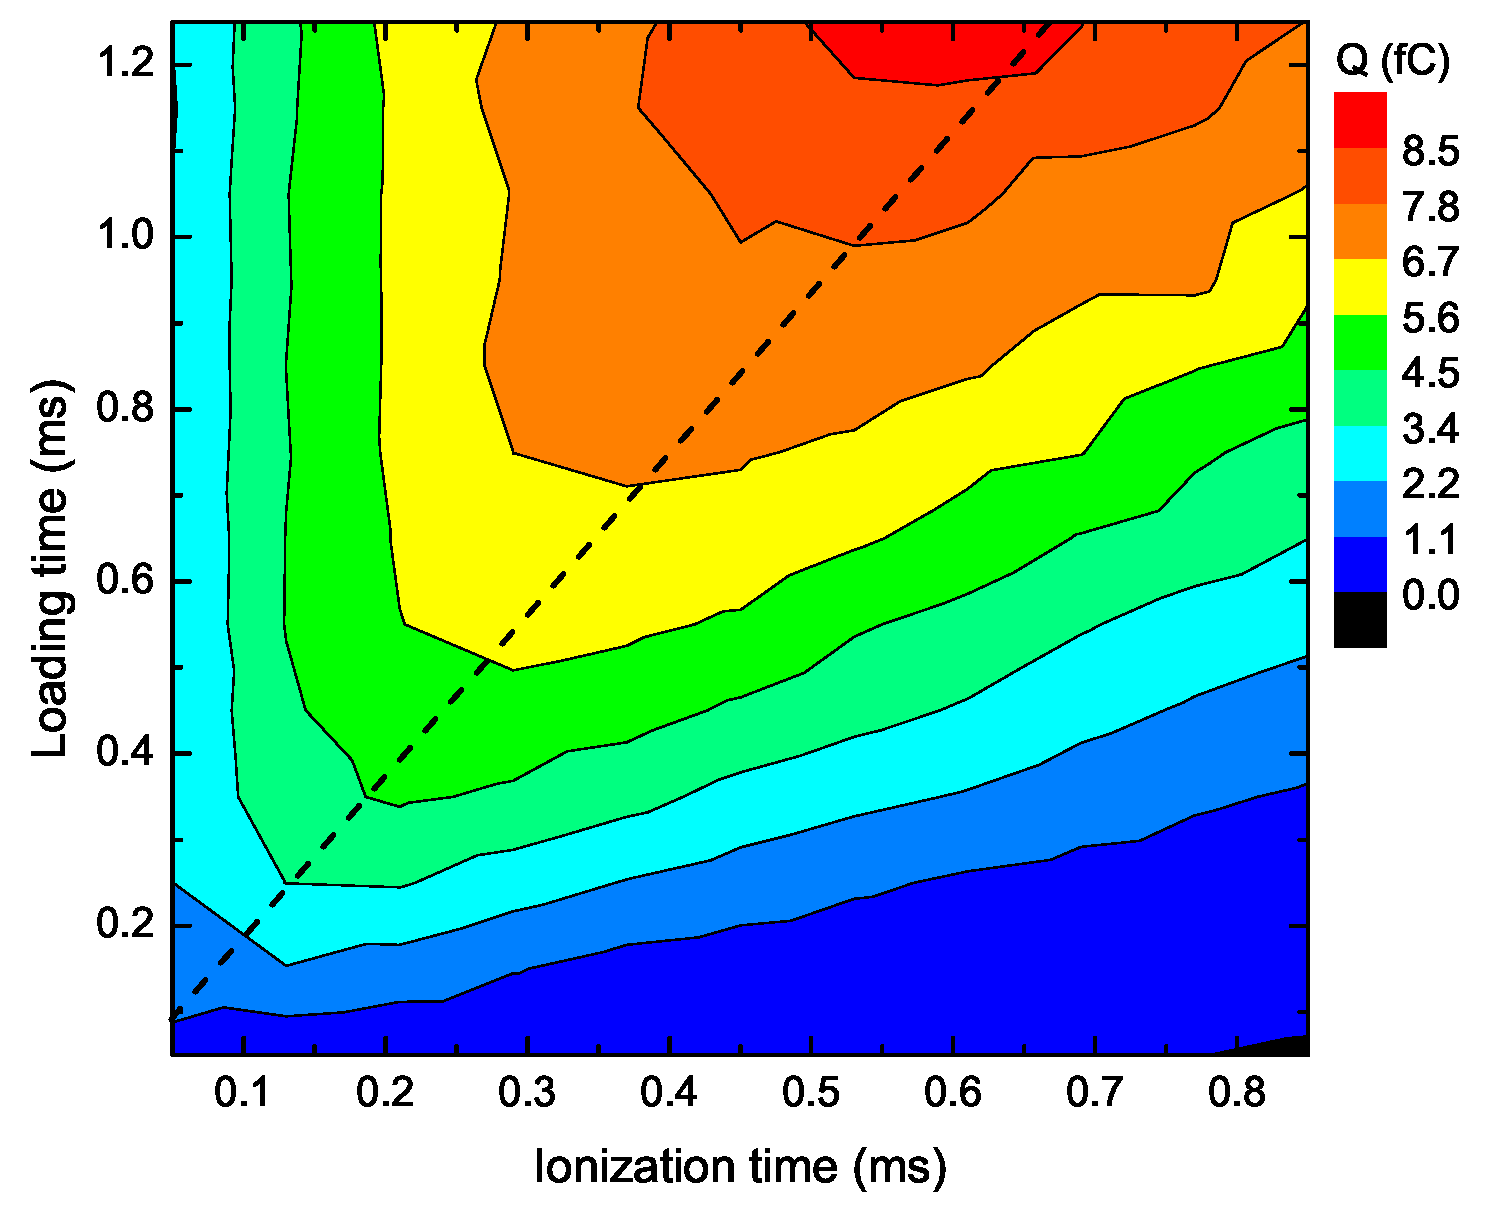
\includegraphics[width=0.6\linewidth]{pics/currmea/2DPlotChargeS=12.eps}
    \caption{Contour plot of the charge per pulse for $s_0=12$. Loading for a longer time leads to a larger charge, while ionizing for a longer time is not always beneficial.}
    \label{fig:charge2Dplot}
\end{figure}
The maximum in this graph is 8.8 fC, which corresponds to $5.5 \times 10^4$ ions. In general, longer loading and ionization times increase the charge per pulse, but the graph shows that there is a limit. In general, at a given loading time, increasing the ionization time will reduce the charge since a too long ionization time eventually reduces the available time to load atoms in the trap. The slope $\rho$ can also be defined for charge plots in a similar way as discussed in section \ref{sec:model} for the average current. In this case, $\rho=1.9$ (dashed line in the plot). The ratio is slightly smaller than for the average current of figure \ref{s2}. This is to be expected since a longer ionization time will result in some extra charge, but the period $t_{cycle}$ will be longer, reducing the average current. But since the slope is very similar, optimization of the average current coincides with optimization of the charge per pulse.\\

\noindent {\bf Ionization power dependence.} The power of the ionization laser beam used in the experiments is so small that removal of atoms by ionization can be neglected when determining the number of atoms in the core region. A change in the laser power therefore should not change the temporal behavior of the current pulses but just the number of ionized atoms. Figure \ref{fig:diffP} shows two contour plots from an experiment where the ionization laser power has been decreased by a factor 3.8 with the use of a neutral density filter.
\begin{figure*}[tbh!]
	\subfloat[$P_i=46$ mW\label{p1}]{\includegraphics[width=0.48\linewidth]{pics/currmea/2DPlotBigVolume}}
	\hfill	
	\subfloat[$P_i=12$ mW\label{p2}]{\includegraphics[width=0.48\linewidth]{pics/currmea/2DPlotBigVolumeQuarterIonisPower.eps}}
	\caption{Contour plots of the average current for two different values of the ionization laser beam power. The optimal slope $\rho$ is shown as a dashed line in the figure. A black dot marks the maximum of the average current.\label{fig:diffP}}
\end{figure*}
Here, the size of the core region in the three dimensions is $(39 \times 63 \times 71)$ $\mu$m$^3$ resulting in a volume $V_c=2.8 \times 10^{-12}$ m$^3$. Also, $t_l$ is incremented in steps of 150~$\mu$s between 50~$\mu$s and 1250~$\mu$s and $t_i$ ranges between 50 and 500 $\mu$s in steps of 75 $\mu$s, in total the scan consists of 63 points. As predicted, the shape of the contour in the two figures is very similar and the average current decreased by a factor of 4.1, similar to the decrease in laser power.\\

\noindent {\bf Summary plots.} In this section, two summary plots for several measurements performed with a core volume $V_c=2 \times 10^{-13}$ m$^3$ are presented. In figure \ref{fig:slopes}, the slopes $\rho$ at which the optimum of the average current occurs, are plotted versus the saturation parameter of the excitation laser beam.
\begin{figure}[tbh!]
    \centering
        \includegraphics[width=0.65\linewidth]{pics/currmea/SlopesVsS.eps}
    \caption{Compilation of the slopes from all the experiments done with $V_c=2.8 \times 10^{-12}$ m$^3$. Qualitatively, a larger saturation parameter corresponds to a larger slope.}
    \label{fig:slopes}
\end{figure}
When more measurements are available for a specific $s_0$, they correspond to measurements done at different ionization power. The large uncertainty bars are related to the linear fit not matching the real behavior perfectly, as $\rho$ is not a constant in practice. For this reason the plot is qualitative. It does appear, however, that the slope increases with increasing saturation parameter in agreement with the prediction of section \ref{sec:typcurrent} shown in figure \ref{fig:smallVdiffs}. In general, for increasing saturation parameter, a larger increase in the peak current is expected compared to an increase in the final current. Hence, the gain in charge obtained by ionizing for a longer time is offset by a reduction in the number of atoms if the loading time is not adjusted, so that it is instead beneficial to reduce the ionization time. This then leads to a higher optimal slope $\rho$.

In figure \ref{fig:peakcurrent}, the peak current is plotted versus the saturation parameter. A higher saturation parameter of the excitation laser beam means a higher excited state fraction and therefore a higher initial peak current. Hence, the expected behavior of the peak current is to be proportional to the excited state fraction: $I_{peak} \propto f(s_0,\delta~\rightarrow~0)$, from equation (\ref{eq:fraction}).
\begin{figure}[tbh!]
    \centering
        \includegraphics[width=0.7\linewidth]{pics/currmea/PeakCurrent.eps}
    \caption{Compilation of the peak current (on the left vertical axes) plotted versus the saturation parameter for several experiments with a core size $V_c=2.8 \times 10^{-12}$ m$^3$ and $P_i=46$~mW. The excited fraction $f(s_0,\delta \rightarrow 0)$ (on the right vertical axis) versus $s_0$ is plotted as a solid line.}
    \label{fig:peakcurrent}
\end{figure}
This relation is also plotted in the figure as a solid line. The shape of the curve indeed corresponds to the trend of the data points.

\section{Discussion and conclusion} \label{sec:conclusion}
To summarize, in this paper we described a semi-analytic model that allows one to calculate the current that can be extracted from an ultracold ion source under pulsed operation. An important feature of the model is that it takes into account the radiation pressure exerted by the excitation laser beam. This turns out to have an important influence on the magnitude and temporal behavior of the current because it pushes atoms through the ionization region. The model was used to predict the optimum settings of ionization and loading times to achieve maximum cycle-averaged current. Measurements of extracted currents show general agreement with the predictions in terms of temporal behavior, magnitude of the current, dependence on the position of the ionization volume, and loading and ionization times for which optimum current extraction is achieved. The key parameters of the model, i.e. the temperature of the atoms, the loading rate and lifetimes of the trap, were obtained from auxiliary experiments.  

For a core volume $V_c=2 \times 10^{-13}$ m$^3$, the maximum cycle-average current we obtained was $\overline{I}=(13 \pm 1)$~pA at $t_i=135$ $\mu$s and $t_l=250$ $\mu$s and $s_0=4$. This corresponds to a current density $J= \overline{I}/(2 \pi \sigma_x \sigma_y) = 4.9$ $10^{-3}$ A/m$^2$, where $\sigma_x=21~\mu$m and $\sigma_y = 20~\mu$m. If we assume that the transverse velocity spread of the ions is simply given by the temperature of the trapped atoms as found by Hanssen \emph{et al.} \cite{Hanssen_NL_08}, the transverse reduced brightness of the source is $B_r = Je/\pi k_b T_s= (8 \pm 1) \times 10^4$~A/m$^2$~sr~eV. This not far from the brightness of $3\times 10^5$~A/m$^2$~sr~eV we predicted as ultimately achievable in \cite{Geer_JoAP_07}, but it is obtained for an atom number density that is 40 times lower and a smaller ionization probability per atom than used in that estimate. This again illustrates the beneficial effect of the radiation pressure of the excitation laser beam, which effectively increases the atom number density in the core by a factor of $\sqrt{10}$ in each phase-space planes.

From the size of the ionization laser beam in the $z$-direction $\sigma_{i,z}=31$ $\mu$m and $V_a=800$ V, we calculate an \emph{rms} energy spread of the ion beam $\sigma_U=e \sigma_{i,z} E_0= 0.9$~eV, well below that of the LMIS, for an acceleration field $E_0=V_a/d_{eff}=29$ kV/m with $d_{eff}=27$~mm the effective length of the accelerator \cite{Taban_PRSAB_08}.

The brightness we estimate above is only an upper limit since the transverse velocity spread of the ion beam was not measured. At least two effects could lead to a higher temperature of the ions: heating of the atoms due scattering of the excitation beam, and heating of the ions due to Coulombic interactions \cite{Geer_JoAP_07,Steele_JAP_11}. First, acceleration of the atoms by the excitation beam for $t_i=135$ $\mu$s results in a velocity $v_z=4.61$~m/s and requires every atom to scatter $b\approx$~773 photons. This would lead to a transverse velocity spread equivalent to a temperature of $\sigma_T=(2b/3)T_r=191~\mu$K, where $T_r=0.37~\mu$K is the recoil temperature for Rb-85 \cite{Metcalf_Book_99}. This is comparable to the measured equilibrium temperature of the trapped atoms and should therefore have only a small effect on the source brightness.

Van der Geer \emph{et al} \cite{Geer_JoAP_07} and Steele \emph{et al.} \cite{Steele_JAP_11} have studied heating of ions extracted from a UCIS/MOTIS. For the current density we report here, these calculations indicate that Coulombic effects could have a significant influence for an acceleration field of 29~kV/m. We have therefore simulated extraction of the ions with the {\sc GPT} particle tracking code \cite{gpt} under conditions similar to the experiment. Here we assume a continuous atomic beam characterized by a Gaussian transverse density profile with 20~$\mu$m \textit{rms}-radius, traveling at 5~m/s and subject to an ionization rate with spatial variation according to a Gaussian with 31~$\mu$m \emph{rms} width. The 50\% reduced brightness \cite{Geer_JoAP_07} of the ion beam is calculated at a distance of 0.1~m behind the ionization region. The resulting reduced brightness of the ion beam is shown as a function of extracted current in figure~\ref{fig:GPTresult}, which shows that stochastic heating already decreases brightness starting at currents as low as 1~pA (solid curve in black). Since in the experiment peak currents of 50~pA are obtained, stochastic heating will be a dominating influence. To reduce the effect, the peak current should be reduced by operating the source in a continuous mode, and the magnitude of the accelerating field increased. To preserve the 1~eV energy spread, the ionization laser beam could be more narrowly focused. To exploit at best the pushing effect, the ionization laser beam can be moved to immediately behind the MOT in the positive $z$-direction (see figure~\ref{fig:setup}). The solid line in red in figure~\ref{fig:GPTresult}, show the case where an higher extraction voltage, $V_a=4$~kV, is used, leading to a higher energy spread $\sigma_U = 4.5$~eV. The energy spread is similar to the one of the LMIS and in under those circumstances the disorder induced heating is ignorable up to 10 pA extracted current.

\begin{figure}[tbh!]
    \centering
        \includegraphics[width=0.7\linewidth]{pics/currmea/GPTresult.eps}
    \caption{Simulated ion beam brightness as function of extracted current for conditions similar to the experiment. Dashed curves: Coulombic interactions excluded; solid curve: included (for two different energy spread values).}
    \label{fig:GPTresult}
\end{figure}
 
One conclusion we draw from the model is that the currently available ionization power of $P_i=46$~mW is insufficient to ionize all the atoms that pass through the ionization volume. Therefore it is possible to extract more current from the source by using a more intense ionization laser beam. To calculate this current, an extension of the model discussed in section \ref{sec:model} is required since the assumption above equation~\ref{eq:current} is no longer valid for a large $P_i$. In this extension of the model, the number of atoms will be corrected for the fraction of the atoms that have been ionized, $C_i$. In order to keep the calculation simple, this fraction is calculated as though the atoms move at a constant velocity in the core volume, resulting in
\begin{equation}
	C_i(t,z) = \exp\left(-r_i \cdot f(s_0,\delta(v_z)) \cdot \min\left(\frac{z+ \sigma_i \sqrt{\pi/2}}{v_z},t\right)\right).
  \label{eq:aveN2}
\end{equation}
The time spent in the core is limited to at most the time that the ionization laser beam is on. We can include depletion of the number of atoms by inserting the factor $C_i(t,z)$ in the integral in both equations (\ref{eq:Ncorecyl_unsolved}) and (\ref{eq:diffin2}). Figure \ref{fig:highpower} plots the calculated temporal dependence of the current for $P_i=$ 0.05, 0.5 and 5 W at $s_0=5$. 
\begin{figure}[tbh!]
    \centering
        \includegraphics[width=0.7\linewidth]{pics/currmea/ModelHighIonisPower}
    \caption{A plot of the behavior of the modeled current in logarithmic scale over time for three different values of the ionization laser beam power with a saturation parameter $s_0=5$ of the excitation laser beam.}
    \label{fig:highpower}
\end{figure}
At large ionization power, the core region is quickly depleted so that the initial current is very large but decays in a very short time. After a while the current increases again due to the contribution of atoms pushed into the core region until it finally decreases to a steady level. For  large laser power, the temporal behavior of the current therefore does not resemble an exponential decay anymore. After optimizing loading and ionization times, we find that a maximum average current of $\overline{I} \approx 90$~pA should be possible at large power, $\approx$~7 times larger than for the current $P_i=0.05$ W. Even larger currents should be possible if the ionization volume is enlarged. However, at his point we run into another limitation of the model, which implicitly assumes that the extracted current represents only a small fraction of the loading rate of the trap, which corresponds to 190~pA. If this condition is violated, the atom number density in the trap (equation~\ref{eq:aveN}) is reduced by a substantial loss of atoms due to ionization, leading to lower than predicted currents. In practice this limitation could be overcome by increasing the rubidium vapor pressure, thereby increasing the loading rate. 


%\section{ACKNOWLEDGMENTS}
%The authors thank J. van de Ven, A. Kemper, W. Kemper, L. van Moll, E. Rietman, I. Koole and H. van Doorn for technical support. This research is supported by the Dutch Technology Foundation STW, applied science division of the ``Nederlandse Organisatie voor Wetenschappelijk Onderzoek (NWO)'' and the Technology Program of the Ministry of Economic Affairs.\\

\clearpage

\begin{subappendices}

\section{Extension to the DC source (UCIS$^+$)} \label{sec:extra}

Here we investigate operation of the source in DC mode as illustrated in figure~\ref{fig:source_CW}, in order to extract even higher beam currents.
\begin{figure}[tbh!]
    \centering
        \includegraphics[width=0.55\linewidth]{pics/currmea/source_CW}
    \caption{Schematic representation of the UCIS$^+$, not to scale. Differently than in figure \ref{fig:source}, the ionization lase beam is translated by $\delta z$ to better exploit the pushing effect of the excitation laser beam. An aperture is added to the setup.}
    \label{fig:source_CW}
\end{figure}
Differently than in figure \ref{fig:source}, the ionization lase beam is positioned at a positive distance $\delta z$ from the center of the MOT, to better exploit the pushing effect of the excitation laser beam. The power of the ionization laser beam is set at 5 W and the source is then renamed UCIS$^+$.

\begin{figure}[tbh!]
    \centering
        \includegraphics[width=0.6\linewidth]{pics/currmea/newsource08}
    \caption{The current $I_{DC}$ plotted versus $\sigma_i$ and $s_0$.}
    \label{fig:newsource}
\end{figure}

The approach is different from the one described in section \ref{sec:model}. The velocity $v_z$ of a particle being pushed by the excitation laser after a time $t$ is given by equation (\ref{eq:velocity}). The distance traveled by the particle is calculated from
\begin{equation}
	d(v_z) = \int_0^{v_z} \frac {v'_z} {a} d v'_z = \frac{m v_z^2}{\Gamma \hbar} \left( \frac{1}{k} + \frac{1}{k s_0} + \frac{2 k v_z^2}{\Gamma^2 s_0} \right),
  \label{eq:distance2}
\end{equation}
where the acceleration $a=F/m$ and the force $F$ are defined in equation (\ref{eq:force}). The current distribution is
\begin{equation}
	\frac{\partial I}{\partial v_z} = \frac{\partial I}{\partial d} \frac{\partial d}{\partial v_z} = K e^{\left( -(d(v_z)-\Delta z)^2 / {2 \sigma_M^2} \right)} e^{-t/\tau_d} \frac{v_z}{a},
  \label{eq:Idv}
\end{equation}
with $K=e \pi \sigma_e n_c \langle v \rangle  / \sqrt2$ including all constants and $\partial d/\partial v_z = v_z/a$ is calculated by derivation of equation \ref{eq:distance2} with respect to the velocity. The quantities $\langle v \rangle=0.3$ m/s, $n_c=2.5 \times 10^{16}$~m$^{-3}$ and $\delta z=\sigma_M =0.8$ mm are used for the calculations. The DC current extracted from the UCIS$^+$ $I_{DC}$ is then given by
\begin{equation}
	I_{DC} = \int_0^{v_z(t_{\infty})}{\frac{\partial I}{\partial v_z}} \left( 1 - p_s \right) d v,
  \label{eq:CWcurrent}
\end{equation}
where $p_s$ is the probability for a particle to ``survive'' the ionization process and is given by
\begin{equation}
	p_s=e^{-f r_i \sqrt{2 \pi} \sigma_i/v_z}.
  \label{eq:prob}
\end{equation}
The ionization rate is defined as in equation (\ref{eq:r_ion}) and the excited state fraction is $f=0.5$, since the trapping laser beams are always turned on.

Figure \ref{fig:newsource} show the current $I_{DC}$ plotted versus the excitation laser beam radius $\sigma_e$ and the saturation parameter of the excitation laser beam $s_0$. %, for $\Delta z=0,~\sigma_m,~2 \sigma_M$.
%\begin{figure*}[tbh!]
%	\subfloat[$\Delta z=0$ mm\label{cw1}]{\includegraphics[width=0.48\linewidth]{pics/newsource0}}
%	\hfill	
%	\subfloat[$\Delta z=\sigma_M$\label{cw2}]{\includegraphics[width=0.48\linewidth]{pics/newsource08}}
%	\hfill
%	\centering	
%	\subfloat[$\Delta z=2 \sigma_M$\label{cw3}]{\includegraphics[width=0.48\linewidth]{pics/newsource16}}
%	\caption{The current $I_{DC}$ plotted versus $\sigma_i$ and $s_0$, for three values of $\Delta z$ (expressed in unit of $\sigma_M=0.8$ mm).\label{fig:newsource}}
%\end{figure*}
%From the results, it can be seen that the highest current are obtained at $\delta z = \sigma_M$. For a larger $\delta_z$, the diffusion out of the atoms outside of the cylinder becomes more important. Currents in the order of 100 pA can be extracted from the UCIS$^+$. This is achieved for instance using $s_0=1$ and $\sigma_e=100~\mu$m, which is still much smaller than $\sigma_M=0.8$ mm.\\
From the results, it can be seen that the highest current in the order of 100 pA can be extracted from the UCIS$^+$. This is achieved for instance using $s_0=1$ and $\sigma_e=100~\mu$m, which is still much smaller than $\sigma_M=0.8$ mm.
Disorder induced heating will still probably reduce the brightness as shown in figure \ref{fig:GPTresult} under the same conditions, but no simulation with GPT has been performed.

\end{subappendices}

\clearpage

\bibliographystyle{unsrt}
%
\begin{thebibliography}{10}

\bibitem{itrs}
http://www.itrs.net/.

\bibitem{Moore_E_65}
G.E. Moore.
\newblock {C}ramming more components onto integrated circuits.
\newblock {\em Electronics}, 38/8, 1965.

\bibitem{Hagen_J_08}
C.~W. Hagen, E.~Fokkema, and P.~Kruit.
\newblock {B}rightness measurements of a gallium liquid metal ion source.
\newblock {\em J Vac Sci Technol B}, 26(6):2091--2096, 2008.

\bibitem{Bell_JVSTB_88}
A.E. Bell, K.~Rao, G.A. Schwind, and L.W. Swanson.
\newblock {\em J. Vac. Sci. Technol. B}, 6:927--931, 1988.

\bibitem{Volkert2007}
C.~A. Volkert and A.~M. Minor.
\newblock Focused ion beam microscopy and micromachining.
\newblock {\em MRS Bulletin}, 32:389--399, 2007.

\bibitem{Kruit_NIaMiPRSAASDaAE_95}
P.~Kruit, L.~J. Vijgen, and Jiang Xinrong.
\newblock {C}oulomb interactions in microfocussed electron and ion beams.
\newblock {\em Nuclear Instruments and Methods in Physics Research Section A:
  Accelerators, Spectrometers, Detectors and Associated Equipment},
  363(1-2):220 -- 224, 1995.

\bibitem{Hanssen_PRA_06}
J.~L. Hanssen, J.~J. McClelland, E.~A. Dakin, and M.~Jacka.
\newblock {L}aser-cooled atoms as a focused ion-beam source.
\newblock {\em Phys. Rev. A: At. Mol. Opt. Phys.}, 74(6):063416, Dec 2006.

\bibitem{Geer_JoAP_07}
S.~B. van~der Geer, M.~P. Reijnders, M.~J. de~Loos, E.~J.~D. Vredenbregt,
  P.~H.~A. Mutsaers, and O.~J. Luiten.
\newblock {S}imulated performance of an ultracold ion source.
\newblock {\em J. Appl. Phys.}, 102(9):094312, 2007.

\bibitem{Metcalf_Book_99}
H.J. Metcalf and P.~van~der Straten.
\newblock {\em {L}aser {C}ooling and {T}rapping}.
\newblock Springer, 1999.

\bibitem{Steele_JVSTB_10}
A.~V. Steele, B.~Knuffman, J.~J. McClelland, and J.~Orloff.
\newblock {F}ocused chromium ion beam.
\newblock {\em J Vac Sci Technol B}, 28(6):C6F1--C6F5, 2010.

\bibitem{Reijnders_PRL_09}
M.~P. Reijnders, P.~A. van Kruisbergen, G.~Taban, S.~B. van~der Geer, P.~H.~A.
  Mutsaers, E.~J.~D. Vredenbregt, and O.~J. Luiten.
\newblock {L}ow-{E}nergy-{S}pread {I}on {B}unches from a {T}rapped {A}tomic
  {G}as.
\newblock {\em Phys. Rev. Lett.}, 102(3):034802, Jan 2009.

\bibitem{Hanssen_NL_08}
J.~L. Hanssen, S.~B. Hill, J.~Orloff, and J.~J. McClelland.
\newblock {M}agneto-{O}ptical-{T}rap-{B}ased, {H}igh {B}rightness {I}on
  {S}ource for {U}se as a {N}anoscale {P}robe.
\newblock {\em Nano Lett.}, 8(9):2844--2850, September 2008.

\bibitem{Debernardi_JAP_11}
N.~Debernardi, M.P. Reijnders, W.~J. Engelen, T.~T.~J. Clevis, P.~H.~A.
  Mutsaers, O.~J. Luiten, and E.~J.~D. Vredenbregt.
\newblock {M}easurement of the temperature of an ultracold ion source using
  time-dependent electric fields.
\newblock {\em J. Appl. Phys.}, 110:024501, 2011.

\bibitem{Steele_JAP_11}
A.~V. Steele, B.~Knuffman, and J.~J. McClelland.
\newblock {I}nter-ion coulomb interactions in a magneto-optical trap ion
  source.
\newblock {\em J. Appl. Phys.}, 109(10):104308, 2011.

\bibitem{Reijnders_PRL_10}
M.~P. Reijnders, N.~Debernardi, S.~B. van~der Geer, P.~H.~A. Mutsaers, E.~J.~D.
  Vredenbregt, and O.~J. Luiten.
\newblock {P}hase-{S}pace {M}anipulation of {U}ltracold {I}on {B}unches with
  {T}ime-{D}ependent {F}ields.
\newblock {\em Phys. Rev. Lett.}, 105(3):034802, Jul 2010.

\bibitem{Reijnders_JAP_11}
M.~P Reijnders, N.~Debernardi, S.B. van~der Geer, P.H.A. Mutsaers, E.J.D.
  Vredenbregt, and O.J. Luiten.
\newblock {T}ime-dependent manipulation of ultracold ion bunches.
\newblock {\em J. Appl. Phys.}, 109:033302, 2011.

\bibitem{Foot_Book_05}
C.~J. Foot.
\newblock {\em {A}tomic {P}hysics}.
\newblock Oxford University Press, 2005.

\bibitem{Taban_PRSAB_08}
G.~Taban, M.~P. Reijnders, S.~C. Bell, S.~B. van~der Geer, O.~J. Luiten, and
  E.~J.~D. Vredenbregt.
\newblock {D}esign and validation of an accelerator for an ultracold electron
  source.
\newblock {\em Phys. Rev. Spec. Top. Accel Beams}, 11(5):050102, 2008.

\bibitem{Monroe_PRL_90}
C.~Monroe, W.~Swann, H.~Robinson, and C.~Wieman.
\newblock {V}ery cold trapped atoms in a vapor cell.
\newblock {\em Phys. Rev. Lett.}, 65(13):1571--1574, Sep 1990.

\bibitem{Gabbanini_OC_97}
C.~Gabbanini, S.~Gozzini, and A.~Lucchesini.
\newblock {P}hotoionization cross section measurement in a {R}b vapor cell
  trap.
\newblock {\em Optics Communications}, 141(1-2):25 -- 28, 1997.

\bibitem{Weiss_JB_89}
D.S. Weiss, E.~Riis, Y.~Shevy, P.J. Ungar, and S.~Chu.
\newblock {O}ptical molasses and multilevel atoms: experiment.
\newblock {\em JOSA B}, 6:2072--2083, 1989.

\bibitem{gpt}
http://www.pulsar.nl/gpt.

\end{thebibliography}

%
%\end{document}

 \chapter[High brightness ion beam through MOC]{High brightness ion beam through magneto-optical compression\label{ch:newsource}}
%\documentclass [10pt,a4paper] {article}
%\documentclass[aip,jap,twocolumn,preprint,showpacs]{revtex4}
%\documentclass[aip,jap,reprint,twocolumn,showpacs,floatfix]{revtex4-1}
%\documentclass[]{iopart}
%
%\usepackage{graphicx}% Include figure files
%\usepackage{dcolumn}% Align table columns on decimal point1
%\usepackage{bm}% bold math
%\usepackage[caption=false]{subfig}
%%\usepackage{subfigure}  % use for side-by-side figures
%
%% to solve conflict between ansmath and iopart
%\expandafter\let\csname equation*\endcsname\relax						
%\expandafter\let\csname endequation*\endcsname\relax
%
%\usepackage{amsmath}	% split equations in more lines
%%\usepackage[OPTIONS]{preview}
%
%\begin{document}

%\title{High brightness ion beam through magneto-optical compression}
%
%\author{N Debernardi, R P M J W Notermans, D J N Kusters, S B van der Geer, P H A Mutsaers, O J Luiten and E J D Vredenbregt}
%\address{Department of Applied Physics, Eindhoven University of Technology, P.O Box 513, 5600 MB Eindhoven, the Netherlands}
%\ead{E.J.D.Vredenbregt@tue.nl}
%
%\date{\today{}}

\begin{abstract}
We show that the combination of a high flux atomic beam originating from a Knudsen cell and the technique of magneto-optical compression, can be used to create an extremely bright ion beam with a low longitudinal energy spread. Realistic simulations of laser cooling and ion beam formation are reported, taking into account the effect of disorder-induced heating. This research shows that a reduced brightness on the order of $10^7$~A/m$^2$~sr~eV with an ion current of tens of pA and an energy spread of about 1 eV can be achieved with a $^{87}$Rb$^+$ beam. This is possible when the so called pencil-beam regime is reached, where the beam size is smaller than the transverse inter-particle spacing.
\footnote{The work described in this chapter by \underline{N. Debernardi}, R P M J W Notermans, D J N Kusters, S B van der Geer, P H A Mutsaers, O J Luiten and E J D Vredenbregt has been submitted for publication to New J. Phys.}
\end{abstract}

\clearpage

\section{Introduction}
Focused Ion Beams (FIBs) are widely used in the semiconductor industry. The properties of the ion source that is implemented in the FIB ultimately limit the characteristics of the beam. The current state-of-art is the Liquid-Metal Ion Source (LMIS), which has a longitudinal energy spread of 4.5 eV and a reduced brightness of $10^6$~A/m$^2$~sr~eV \cite{Orloff_RoSI_93}. The minimum spot size that can be achieved with a LMIS is limited by the chromatic aberration due to the relatively large longitudinal energy spread of the source. Alternative sources, that combine a lower energy spread with a comparable or even a higher brightness, are needed to enable further development of FIBs to keep up with the trend of the production of smaller and smaller semiconductor components \cite{Moore_E_65}.

In previous work \cite{Debernardi2012, Reijnders_PRL_09}, the properties of an ion beam extracted from an ultracold ion source (UCIS) have been investigated. $^{85}$Rb atoms were collected, cooled down in a magneto-optical trap (MOT), and subsequently photo-ionized. In this way, ion bunches are extracted and accelerated with a high repetition rate. An upper limit for the reduced brightness was set at $8 \times 10^4$~A/m$^2$~sr~eV, but simulations showed that disorder-induced heating does reduce the brightness by one to two orders of magnitude, depending on the extracted current. The brightness of a MOT-based source therefore remains far below that of the LMIS. The strength of the UCIS, and of similar sources as the MOTIS \cite{Hanssen_PRA_06, Hanssen_NL_08}, is in its versatility, since several different atomic species can be used \cite{Steele_JVSTB_10}. Moreover, energy spread down to 20 meV has been demonstrated \cite{Reijnders_PRL_09}, substantially lower than a LMIS.

In this paper, a new source concept with better performance with respect to the UCIS is investigated. The essential difference with the UCIS is that this new source is based on two-dimensional magneto-optical compression of an atomic beam rather than three-dimensional magneto-optical trapping of an atomic vapor. Extending the original idea of Freinkman \textit{et al.} \cite{Freinkman2004}, an atomic beam laser-cooled ion source (ABLIS) is proposed, as schematically shown in figure \ref{fig:setup_newsource}.
\begin{figure}[tbh!]
    \centering
        \includegraphics[width=0.6\linewidth]{pics/newsource/setup4}
    \caption{Schematic drawing of the setup in the $xz$ plane, not to scale. From the left to the right hand side, an atomic beam $B$, formed from an aperture $S$ of a Knudsen cell $K$, is skimmed by an aperture with area $A_i$. In the MOC, the beam is cooled with 2 pairs (in the drawing only one pair is shown) of counter-propagating laser beams perpendicular to the z-axis (with $\sigma^+$ and $\sigma^-$ polarization) and, at the same time, it is compressed with a magnetic gradient $G$ into an aperture with area $A_f$. The quantities $d$ and $d_f$ represents either the aperture radius (for the analytical model) or the half-width aperture size (for the simulations). The distance between $A_i$ and $A_f$ is $L$. The aperture $A_f$ is put at a positive potential. Finally, the beam is ionized and an ultracold ion beam $U$ is created. The ionization process occurs in an electric field so that the beam is also accelerated toward the last aperture $H$ which is grounded.} 
    \label{fig:setup_newsource}
\end{figure}
The setup can be divided in three parts: in the first part, an atomic beam $B$ is formed by skimming with an aperture of area $A_i$ the expansion of a gas or vapor emanating from a Knudsen cell with an aperture of area $S$. In the second part, the beam is cooled down transversally by two pairs of counter-propagating laser beams and simultaneously compressed in the presence of a magnetic field gradient. This component is named MOC (Magneto-Optical Compressor). In the third part, after passing through a second aperture with area $A_f$, the atomic beam is crossed with an ionization laser beam in an electric field and an ultracold ion beam $U$ is then created. The second aperture is put at a positive potential and the anode $H$ is grounded, so that the electric field $\vec{E}$ accelerates the ions toward $H$. The quantities $d$ and $d_f$ represent either the aperture radius (for the analytical model) or the half-width aperture size (for the simulations). 

Very large gains in atomic beam brightness have been obtained with laser cooling methods in the past \cite{Tempelaars2002, Lison1999}. However, this required extensive beam lines that are impractical for mounting on a FIB column. Here we investigate what brightness a compact setup involving only a source and short compressor can deliver. The ABLIS exploits a high atomic flux that effuses from a Knudsen cell and converts, cools and compresses it into a micrometer range transverse beam size with milliKelvin transverse temperature, greatly increasing its brightness. By restricting the diameter of the atomic beam with aperture $A_f$, before the atoms are converted to ions, the so-called ``pencil-beam'' regime \cite{Tiemeijer1999} can be reached: space charge forces in the transverse direction are negligible and the brightness should be less influenced by disorder-induced heating.

This paper first presents an analytical model which can be used to predict the general dependence of the source performance on some key variables. The reduced brightness and the current are examples of the source properties that will be calculated. Secondly, this model is used for a preliminary optimization and as a starting point for particle tracing simulations, which are required in order to include a more realistic physics and to avoid limitations of the model. Several simulations of the intensification of the atomic beam MOC are calculated with the computer code COOL~\cite{Vredenbregt_AJoP_03}, which treats Doppler cooling \cite{Metcalf_Book_99} of individual atoms in magnetic fields. The best case scenario is then used as input for simulations of the ion beam formation using the General Particle Tracer code (GPT) \cite{gpt}, which treats the motion of ions in external electromagnetic fields where the Coulomb interaction between ions is taken into account. Finally, it is shown that, according to the simulations, this source can achieve both a higher brightness and a lower energy spread than LMIS, at the same time.

\section{Analytical model of the source}\label{sec:anamodel}
An analytical model is developed in order to estimate the performance of the source and to have a starting point for the optimization in the parameter space of several variables, before performing simulations. The  model is based on a standard theoretical treatment of laser cooling, such as formulated by Metcalf and Van der Straten \cite{Metcalf_Book_99}.

The flux $\Phi_i$ of atoms emanating from a Knudsen cell with an aperture of area $S$ within a small azimuthal angle $\theta$ and at an atomic density $n$ is given by 
\begin{equation}
    \Phi_i = \frac{1}{4} n S \left\langle v \right\rangle \theta^2.
    \label{eq:flux_i}
\end{equation}
The density $n=p/(k_b T_s)$ of the atoms can be controlled with the temperature $T_s$ of the Knudsen cell, where $k_b = 1.381 \times 10^{-23}$ m$^2$ kg s$^{-2}$ K$^{-1}$ is Boltzmann's constant. For alkali metal vapors above the melting temperature, we can approximate the pressure as $p=p^*\exp(-T^*/T_s)$ \cite{Haynes_Book_12}, where the constants $p^*$ and $T^*$ depend on the atomic element, the physical state and the source temperature, and they can be calculated from reference \cite{Haynes_Book_12}. Table \ref{tab:Rb_atomic_consts} lists the atomic properties of rubidium, which is the atomic species used in this paper.
\begin{table}[h!]
	\centering
	\caption{Atomic constants used in the calculations and the simulations. Note that the values of $p^*$ and $T^*$ are valid for a set of source temperatures ranging from $312$~K (melting point) to $550$~K \cite{Haynes_Book_12}.}
	\begin{center}
		\begin{tabular}{|l|l|l|l|} \hline
		{Parameter (unit)} & {Symbol} & {$^{85}$Rb} & {$^{87}$Rb} \\ \hline
		{Mass (amu)} \cite{Haynes_Book_12_b}& $m$ & {84.91 } & {86.91 } \\ 
		{Pressure constant (Pa)} \cite{Haynes_Book_12}& $p^*$ & {$2.08 \times 10^9$ } & {$2.08  \times 10^9$ } \\ 
		{Temperature constant (K)} \cite{Haynes_Book_12}& $T^*$ & {$9.30 \times 10^3$ }	& {$9.30 \times 10^3$ } \\ 
		{Natural linewidth (MHz)} \cite{Metcalf_Book_99}& $\Gamma/2 \pi$ & {5.98 } & {5.98 }	\\ 
		{Saturation intensity (W/m$^2$)} \cite{Metcalf_Book_99}& $I_s$ & {16.4} & {16.4} \\
		{Abundance (\%)} \cite{Haynes_Book_12_b} & {$ab$} & {72.2} & {27.8}	\\  
		{Cooling wavelength (nm)} \cite{Metcalf_Book_99}& {$\lambda$} & {780} & {780} \\
		{Nuclear spin quantum number} \cite{Haynes_Book_12_b}& $I$ & {$5/2$ } & {$3/2$ }	\\ \hline
		\end{tabular}
	\end{center}
	\label{tab:Rb_atomic_consts}
\end{table}

The longitudinal velocity $v_z$ follows a Maxwell-Boltzmann distribution and its average $\left\langle v \right\rangle$ is related to the source temperature as
\begin{equation}
    \left\langle v \right\rangle = \sqrt{\frac{8 k_b T_s}{\pi m}},
    \label{eq:t_thermal}
\end{equation}
where $m$ is the mass of the atom. \\
The angle is defined as $\theta=d/l$ where $d$ is the aperture size (intended as aperture radius in this analytical model) and $l$ is the expansion stage length between the Knudsen cell and the MOC, as shown in figure \ref{fig:setup_newsource}.\\ 
The flux of equation (\ref{eq:flux_i}) corresponds to a reduced initial brightness $B_r^i$, which can be calculated as \cite{Luiten_IJoMPA_07}
\begin{equation}
    B_r^i = \frac{e J}{\pi k_b T'_s}= \frac{e^2 \Phi_i / S}{\pi k_b T_s \theta^2},
    \label{eq:br_i}
\end{equation}
where $e = 1.602 \times 10^{-19}$~C is the elementary charge and $T'_s=T_s \theta^2$ is the effective source temperature, due to the presence of the initial aperture $A_i$. This is not the brightness of the atomic beam, but an equivalent brightness for an ion beam with the same properties. The extra $e$ factor in the previous equation is necessary to convert the resulting reduced brightness in unit of A/m$^2$~sr~eV. In what follows, the apertures $S$ and $A_i$ are set to be the same size as a simplification in this model.\\

In the second stage, the beam brightness can be increased with the use of a magneto-optical compressor stage. The forces in a MOC are two-dimensional, but we are going to treat the two transverse dimensions as independent, assuming that the total force on an atom can be written as the sum of the radiation pressure of the separate laser beams. Then the problem is quasi-2D. Laser cooling is asserted with two pairs of laser beams, where each pair is made up of two counter propagating laser beams with respectively a $\sigma^+$ and a $\sigma^-$ polarization. Moreover, we consider a transition between two levels with angular momentum quantum numbers $F=0$ and $F=1$. The fact that rubidium has more than one ground state due to hyperfine splitting is ignored, i.e. we assume the presence of a sufficiently strong re-pump laser beam in the experiment. The re-pump laser beam is necessary since the time spent by an atom for traveling in the MOC is about 4 times longer than the average decay time to the wrong ground state. This is calculated using the values shown in table \ref{tab:parametervalues_ana} and the scattering rate formula found in \cite{Metcalf_Book_99}.
\begin{table}[h!]
	\centering
	\caption{Parameter values for a 2-level $^{85}$Rb atom used in the analytical model and the simulation.}
	\begin{center}
		\begin{tabular}{|l|l|l|} \hline
		{Parameter (unit)} & {Symbol} & {Analytical model} \\ \hline
		{Expansion length (m)} & $l$ & {$3.9 \times 10^{-2}$} 	\\ 
		{Initial aperture size (m)} & $d$ & {$3.1 \times 10^{-4}$} 	\\ 
		{Source temperature (K)} & $T_s$ & {$350$} 	\\ 
		{Cooling and compression length (m)} & $L$ & {$5 \times 10^{-2}$} 	\\ 
		{Saturation parameter (-)} & $s_0$ & {$2$} 	\\ 
		{Detuning ($\Gamma$)} & $\delta$ & {$-0.5$} 	\\
		{Magnetic gradient (T/m)} & $G$ & {$1$}	\\ \hline
		\end{tabular}
	\end{center}
	\label{tab:parametervalues_ana}
\end{table}

For one set of counter propagating beams, the force $F_{MOC}$ acting on an atom has the expression \cite{Metcalf_Book_99}
\begin{equation}
    %F = \frac{\hbar k s_0 \Gamma/2}{1 + s_0 + \left( \frac{2 \delta_{eff}}{\Gamma} \right)^2},
    F_{MOC} = \hbar k s_0 \Gamma/2 \left[ \left[1 + s_0 + 4 \left( \delta_{eff}^+ \right)^2 \right]^{-1} - \left[1 + s_0 + 4 \left( \delta_{eff}^- \right)^2 \right]^{-1} \right].
    \label{eq:force_newsource}
\end{equation}
In this equation, $s_0 = I_L/I_s$ is the saturation parameter, with $I_L$ as the laser beam intensity, $I_s$ as the saturation intensity and $\Gamma$ as the natural linewidth of the atomic transition. Moreover, $\delta_{eff}^{\pm}$ is the effective detuning of the laser beam, which is the sum of three terms:
\begin{equation}
    %\delta_{eff}^{\pm} = \delta \pm k v_x \pm \frac{G \mu_b x}{\hbar},
    \delta_{eff}^{\pm} = \delta_n \pm \frac{k v_x}{\Gamma} \pm \frac{G \mu_b x}{\Gamma \hbar},
    \label{eq:detu_eff}
\end{equation}
where $\delta_n=\delta/\Gamma$ is the normalized laser detuning with $\delta$ as the laser detuning in unit of $\Gamma$, $k=2 \pi / \lambda$ is the wave number, $\lambda$ is the laser wavelength, $v_x$ is the transverse velocity of the atom, $G$ is the magnetic field gradient, $\mu_b = 9.27 \times 10^{-24}$~J/T is the Bohr magneton, $x$ is the transversal position of the atom and finally $\hbar = 1.055 \times 10^{-34}$~J~s is Dirac's constant. In equation (\ref{eq:detu_eff}), the positive sign of $\delta_{eff}$ is for a laser beam traveling along the positive $x$-axis direction and the negative one is for a laser beam traveling in the opposite direction.
The force of equation (\ref{eq:force_newsource}) accelerates an atom according to Newton's second law $F_{MOC}=m a$.

The Doppler temperature $T_D$, defined as \cite{Foot_Book_05} 
\begin{equation}
    %T_D = \hbar \Gamma / 2 k_b,
    %T_D = - \frac{\hbar \Gamma}{4 k_B} \Big( \frac{\Gamma}{2\delta}(1 + s_0) + \frac{2 \delta}{\Gamma}\Big),
    T_D = - \frac{\hbar \Gamma}{4 k_b} \Big( \frac{1 + s_0}{2\delta_n} + 2 \delta_n \Big),
    \label{eq:Tdoppler}
\end{equation}
is the minimum temperature reachable with elementary Doppler laser cooling. In order to efficiently cool to the Doppler temperature the atoms passing the first aperture $A_i$, the skimming aperture is sized to transit only atoms whose transverse velocity with respect to the atomic beam axis is smaller than the capture velocity $v_c = -\delta / k$~\cite{Metcalf_Book_99}. In what follows we will keep the maximum transverse velocity at a fixed value of $v_{max}=\Gamma/{2 k}$ which results in a opening angle of $\theta=v_{max}/\left\langle v \right\rangle=8$~mrad, i.e. the nominal value for a detuning of $-\Gamma/2$ (which is the optimum for laser-cooling \cite{Metcalf_Book_99}) and a source temperature of 350~K. This ensures that the transverse velocities of the atoms remain well within the capture range over most of the parameter range that we consider. For larger detunings, the brightness we obtain in this way probably then represents a lower limit that may be further increased by relaxing the criterion. After cooling, the brightness of the atomic beam $B_c$ becomes
\begin{equation}
    B_r^c = B_r^i \frac{T_s~{\theta}^2}{T_D} = \frac{e^2 \Phi / S}{\pi k_b T_D}.
    \label{eq:b_c}
\end{equation}
Using the values of table \ref{tab:parametervalues_ana}, the gain in brightness $T_s~\theta^2/T_D \approx 77$ only due to Doppler cooling is already very large.

With magneto-optical compression, in addition, the beam's area can be reduced, leading to an extra increase in the brightness. Using a compression length $L$ and a corresponding compression time $t$ defined as 
\begin{equation}
    t=L / \left\langle v \right\rangle,
    \label{eq:time}
\end{equation}
atoms from within an area $A_i=\pi d^2$ can be forced into a smaller area $A_f$. The initial aperture size $d$ is calculated with the values shown in table \ref{tab:parametervalues_ana} as \cite{Foot_Book_05}
\begin{equation}
    %d=\frac{a_{max} t^2}{4} = \frac{F L^2}{4 m \left\langle v \right\rangle^2} = 309 \times 10^{-6}~m.
    d=\frac{a_{max} L^2} {4 \left\langle v \right\rangle^2} = 3.1 \times 10^{-4}~\textrm{m},
    \label{eq:init_r}
\end{equation}
where the maximal acceleration is defined as $a_{max}=\lim_{(v_x~\to~v_c,~x~\to~0)}~F_{MOC}/m$.

The initial expansion stage length $l$ is calculated as
\begin{equation}
    l = \frac{d}{\theta} = 3.9 \times 10^{-2}~\textrm{m}.
    \label{eq:init_d}
\end{equation}

The final beam area is calculated assuming that atoms have reached equilibrium as $A_f=\pi k_b T_D/\kappa$. The spring constant $\kappa$ of the previous equation is given by
\begin{equation}
    \kappa = \lim_{v_x \to 0, x \to 0} \Big[ -\frac{\partial F_{MOC}}{\partial x} \Big] = -8 \mu_B G s_0 k \frac{\delta_n}{(1 + s_0 + 4 \delta_n^2)^2}.
    %\kappa = \mu_b G s_0 k,
    \label{eq:spring}
\end{equation}

After the compression the resulting reduced brightness of the atomic beam $B_r^f$ is then expressed as 
\begin{equation}
    B_r^f = B_r^c  \frac{A_i}{A_f} = \frac{e^2 \Phi / S}{\pi k_b T_D} \frac{A_i}{A_f}.
    \label{eq:br}
\end{equation}
We can now calculate the gain in brightness due to compression. From equation (\ref{eq:br}) and substituting the values of table \ref{tab:parametervalues_ana}, it results that $A_i/A_f=d^2 \kappa/k_b T_D \approx 900$. So compressing the beam (i.e. going beyond the ideas of Freinkmann \textit{et al} \cite{Freinkman2004}) gives a very large gain in brightness. The total gain in brightness due to cooling and compressing by using a MOC could result in about $7 \times 10^4$. 
More information on cooling and compressing of atoms can be found in \cite{Metcalf_Book_99, Foot_Book_05}.\\

An analytical solution for the reduced brightness $B_r^{ana}$ can be expressed as
\begin{equation}
\begin{split}
    B_r^{ana} =& -\left[ \frac{e^2 \mu_b \sqrt2~\pi^{5/2}}{k_b^{7/2}} \right] \cdot \left[ \frac{p^* \Gamma^2 \sqrt{m}}{\lambda} \right]\\ 
    &\cdot \left[\frac{G~L^4~s_0^3~\delta_n^7~\exp(-T^*/T_s)}{T_s^{7/2} (1+s_0)^2 (1+s_0+4~\delta_n^2)^4 (1+s_0+16~\delta_n^2)^2} \right].
    \label{eq:ana}
\end{split}
\end{equation}
%Eq. (\ref{eq:ana}) can be further rearranged into
%\begin{align}
%    B_r^{ana} = - \frac{16}{\sqrt{2 \pi^3}} \frac{e^2 \mu_B G s_0 A_i \Delta \theta^2}{\lambda \sqrt{m k_b^5}} \frac{p_0 \exp[-T_0/T_s]}{T_D^2 \sqrt{T_s}} \frac{\delta_n}{(1 + s_0 + 4\delta_n^2)^2}.
%    \label{eq:ana2}
%\end{align}
Equation (\ref{eq:ana}) is made up of three main factors included in square brackets: the first term includes all the numerical and physical constants together; the second term contains the constants which depend on the used atom; the last term contains all the parameters of the model over which we have external control. Equation (\ref{eq:ana}) is useful to see the dependence of the reduced brightness versus the parameters of the model ($L$, $G$, $s_0$, $\delta_n$ and $T_s$). Simulations will explore those parameters more in depth in section \ref{sec:results}.

In order to have a realistic starting point for simulations, we need to choose some values of the parameters since the dependence on $G$, $L$ and $T_s$, does not lead to an optimum for the reduced brightness. The brightness scales linearly with the magnetic gradient field. A magnetic gradient $G = 1$~T/m is chosen such that the spatial capture range is approximately equal to the radius of the aperture. The compression length is really important, since the brightness scales as $L^4$. The compression length is chosen to be 0.05~m in order to keep the setup compact and because that is the maximum size of ordinary optics elements. The source temperature can be increased as long as the mean free path $\Lambda$ of the particles is much larger than the aperture size of the Knudsen cell $d$. The mean free path of a particle is defined as \cite{Blundell_Book_06}
\begin{equation}
    \Lambda = \frac{k_b T_s}{\sqrt2 \pi p (2 r_{vdW})^2},
    \label{eq:mfp}
\end{equation}
where $r_{vdW} = 0.3$~nm is the typical Van der Waals radius for rubidium \cite{Mantina2009}. The quantity $\Lambda$ equals 0.5~m for $T_s=350$~K and it drops rapidly to 21~mm for $T_s=400$~K. A higher source temperature means a higher initial flux, but on the other hand, also the longitudinal velocity increases and this influences the efficiency of the compressor stage.
 
Figure \ref{fig:density} displays the reduced brightness of equation (\ref{eq:ana}) versus the saturation parameter and the normalized detuning in case of a 2-level $^{85}$Rb. For this calculation, the used parameters are summarized in table \ref{tab:parametervalues_ana} (except for the quantities $s_0$ and $\delta_n$ which are varied). Here there is a clear optimum, the maximum of the reduced brightness $B_r^{ana} = 2.1 \times 10^7$~A/m$^2$~sr~eV occurs at $\delta_n = -0.8$ (where $\kappa$ is maximized), and at $s_0 = 2$. From this plot, it is also interesting to note that increasing the laser intensity does not increase the brightness for $s_0 > 2$.
\begin{figure}[tbh!]
    \centering
        \includegraphics[width=0.7\linewidth]{pics/newsource/density}
    \caption{The analytical reduced brightness $B_r^{ana}$, in unit of A/m$^2$~sr~eV, plotted versus the saturation parameter and the normalized detuning in case of a 2-level $^{85}$Rb. The used parameters are shown in table \ref{tab:parametervalues_ana}, except from the quantities $s_0$ and $\delta_n$ which are varied.} 
    \label{fig:density}
\end{figure}


\section{Simulation and analysis} \label{sec:simu}
The result of the analytical model is used as a starting point for the simulations. The analytical model considered an ideal 2-level $^{85}$Rb whereas simulations use a realistic atom.

The simulation is made up of two parts. The program COOL \cite{Vredenbregt_AJoP_03} simulates the laser cooling and compression of the atomic beam effused from a Knudsen cell. The simulation is based on absorption and emission of individual photons, but a re-emitted photon does not interact anymore and it is basically "lost"; in other words, the simulation does not include optical thickness of the media into account. The code is unchanged compared to the version from reference \cite{Vredenbregt_AJoP_03} except for replacing the initial particle distribution with something more appropriate to our geometry, see section \ref{sec:initdistr}. The aperture sizes $d$ and $d_f$ in the simulation are meant as half-width aperture size, since square apertures are here used. The square aperture is chosen instead of a circular one because it is computationally simpler.

Finally, the ion tracing simulations are performed with the General Particle Tracer code (GPT) \cite{gpt}, where space charge forces are fully taken into account.

To summarize our computations in terms of the $z$ coordinate of the beam: a geometrical flux calculation is used for $0<z<l$ (see equation \ref{eq:initflux}), the COOL code is used for $l<z<l+L$ and the GPT code for $z>l+L$.

\subsection{Initial particle distribution} \label{sec:initdistr}
In COOL, the initial velocities and angles of the particles are initialized at the first aperture $A_i$ with a Monte Carlo algorithm, according to an appropriate geometrical boundary condition and the Maxwell-Boltzmann velocity distribution. The spatial distribution at the aperture is uniform since $d \ll l$. We approximate the situation by considering motion in the two transverse dimensions separately. For an initial longitudinal velocity, two simulations are performed, one for the $x$-direction and another one for the $y$-direction.

The longitudinal velocities follow the Maxwell-Boltzmann distribution \cite{Scoles1988}
\begin{equation}
  	f_v(v_z) d v_z = N \sqrt{\frac{2}{\pi}} \frac{v_z^2}{v_{\sigma}^3} \exp \Bigg[ - \frac{1}{2} \Big( \frac{v_z}{v_{\sigma}}\Big)^2  \Bigg] d v_z,   
  	\label{eq:initdistr_vel}
\end{equation}
where $v_{\sigma} = \sqrt{k_b T_s / m}$ is the thermal velocity of the atoms. The longitudinal velocity distribution is normalized to $N$, which is the total number of particles in the simulation. Figure \ref{fig:v_distr} shows an example of a typical velocity distribution obtained with $N=5 \times 10^5$ $^{87}$Rb particles effused at $T_s=400$ K. The distribution is fitted with equation (\ref{eq:initdistr_vel}). The thermal velocity determined from the fit is $(194.7 \pm 0.2)$ m/s and is in good agreement with the calculated value $v_{\sigma} =195$ m/s. %From this we conclude that the number of particles is large enough.
\begin{figure}[tbh!]
    \centering
        \includegraphics[width=0.7\linewidth]{pics/newsource/initVelocityDistrOptimized_Rb-87_500k_400K}
    \caption{Initial particle distribution of $N=5 \times 10^5$ $^{87}$Rb atoms at a temperature of 400 K. The distribution is normalized to $N$. The solid line is a fit of the normalized velocity distribution of equation (\ref{eq:initdistr_vel}).} 
    \label{fig:v_distr}
\end{figure}

After randomly picking an initial position $|x| \leq d$ on the aperture $A_i$, the angle $\alpha$ is then initialized. The angle $\alpha$ is also randomly picked according to the criteria
\begin{equation}
  	-\arctan\left({\frac{d-x}{l}}\right) \leq \alpha \leq \arctan\left({\frac{d+x}{l}}\right).
  	\label{eq:ang_criteria}
\end{equation}
The transverse velocity is then calculated as $v_x=\alpha~v_z$. This procedure is repeated for all the $N$ particles.
%The maximum angle is calculated as $\theta_{max} = 2 d/l$ and the number of particles per unit angle is given by
%\begin{equation}
%  	f_{ang}(\alpha) \rmd \alpha = C_0 (2 d-l~\tan(\alpha)) \rmd \alpha; \ \ \ \ \   0 \leq \alpha \leq \arctan(\theta_{max}),
%  	\label{eq:initdistr_ang}
%\end{equation}
%where $C_0$ is a normalization constant (proportional to the number of particles in the simulation). Similarly a particle distribution function can be derived for $\theta < 0$, and differs only by a minus sign from the previous formula. Since with our geometry $\alpha_{max} \ll 1$, it is possible to simplify the angular distribution as
%\begin{equation}
%  	f_{ang}(\alpha) \rmd \alpha \approx C_0 (2d \mp l~\alpha) \rmd \alpha; \ \ \ \ \   0 \leq |\alpha| \leq \theta_{max}.
%  	\label{eq:initdistr_ang2}
%\end{equation}


\subsection{Source characterization}
In this subsection, the definition of the current and the reduced brightness are given. Depending on the parameters, only a certain number of particles $N_f$ will make it through the final aperture $d_f$ and it is necessary to estimate at first the fraction of the flux that is carried by each particle.

The atomic flux $\Phi_i$ through the first aperture $A_i$ is given by
\begin{equation}
	\Phi_i = \frac{n}{4 \pi} \langle v \rangle \mathcal{F}(d,l),
	\label{eq:initflux}
\end{equation}
where in the case of $l \gg d$ \cite{Notermans2012}
\begin{equation}
%\mathcal{F}(d,l) = 8d \Bigg[ \sqrt{4 d^2 + l^2} \arctan \Bigg( \frac{2d}{\sqrt{4d^2+l^2}} \Bigg) - l \arctan \Bigg( \frac{2d}{l} \Bigg) \Bigg]
%+ 2l^2 \ln \Bigg( \frac{4d^2 + l^2}{\sqrt{8l^2d^2 + l^4}}  \Bigg).
	\mathcal{F}(d,l) = 16 \frac{d^4}{l^2} + o\left(\frac{d^6}{l^4}\right).
\label{eq:G_square}
\end{equation}
%A derivation of Eq. (\ref{eq:G_square}) is shown in the Appendix. 
The quantity $\mathcal{F}(d,l)=9.59 \times 10^{-11}$~m$^2$, using the values of $d$ and $l$ found in table \ref{tab:parametervalues_ana} (the result is valid for a square aperture and it differs only a factor $\pi/4$ from the one obtained with a circular aperture \cite{Notermans2012}). Equation (\ref{eq:initflux}) depends on geometrical variables: the free expansion length $l$ and the aperture size $d$, and on the source temperature $T_s$.

The final current $I(d_f)$ (of an ion beam with the same properties) depends on $d_f$ and it is calculated as
\begin{equation}
	I(d_f) = e~C \sum_{j=1}^{N_f(d_f)}{v_{z,j}^f},
	\label{eq:current_newsource}
\end{equation}
with $N_f$ as the number of particles passing through the final aperture $A_f$ and the normalization constant $C$ given by
\begin{equation}
	C = \frac{\Phi_i}{\sum_{j=1}^{N}{v_{z,j}^i}}.
	\label{eq:norma_flux}
\end{equation}
The quantities $v_{z,j}^i$ and $v_{z,j}^f$ respectively represent the initial longitudinal velocity (at the first aperture $A_i$) and the final longitudinal velocity (at the second aperture $A_f$) of the j-th particle.

The final reduced brightness $B_r(d_f)$ is then given by 
\begin{equation}
	B_r(d_f) = \frac{1}{4 \pi^2} \frac{I(d_f)}{\epsilon_r(d_f)},
	\label{eq:brightness}
\end{equation}
which can be derived from \cite{Luiten2007}. In equation (\ref{eq:brightness}), the reduced emittance $\epsilon_r$ of the beam at a fixed position $z$ is given by \cite{Floettmann2003}
\begin{equation}
	\epsilon_r(d_f) = \epsilon_r^x(d_f) \epsilon_r^y(d_f) \approx [\epsilon_r^x(d_f)]^2 = \frac{m}{2} \left[ \left\langle x^2 \right\rangle \left\langle v_x^2 \right\rangle - \left\langle x~v_x \right\rangle^2 \right],
	\label{eq:emittance}
\end{equation}
where $\langle \rangle$ defines the average over the particle ensemble. In equation (\ref{eq:emittance}), since the two orthogonal directions are independent due to the square geometry, the approximation $\epsilon_r^x \approx \epsilon_r^y$ is used.\\
Figure \ref{fig:BrandI_VSaperture_Rb87} shows the reduced brightness plotted versus the final aperture size $d_f$ in case of $^{87}$Rb, using the parameters shown in table \ref{tab:parametervalues}. 
\begin{equation}
	B_r^p = \frac{1}{4 \pi^2} \frac{I^p}{\epsilon_r^p},
	\label{eq:brightness10}
\end{equation}
where the superscript $p$ denotes that only the 10\% of the particles closest to the \textit{z}-axis are used and $I^p=I/10$. The brightness calculated with equation (\ref{eq:brightness10}) approximates the value for $d_f \to 0$ (which can not be calculated numerically) and from now on it will be named peak brightness.\\
Figure \ref{fig:BrandI_VSaperture_Rb87} also shows the current versus the final aperture size and it can be seen that an aperture size $d_f=1~\mu$m corresponds to about $I=30$~pA. The plot also shows that the current density is constant up to $d_f=5~\mu$m, where a current on the order of 1~nA can be achieved.
\begin{figure}[tbh!]
    \centering
        \includegraphics[width=0.7\linewidth]{pics/newsource/BrandI_VSaperture_Rb87}
    \caption{The reduced brightness $B_r$ at the end of the MOC plotted versus the final aperture size $d_f$ (solid line) on a double logarithmic scale. The dashed line indicates the reduced peak brightness $B_r^p$ as defined in equation (\ref{eq:brightness10}). Also, the current is plotted as a dash-dot line. Both of the curves are obtained with $^{87}$Rb, see table \ref{tab:parametervalues}.} 
    \label{fig:BrandI_VSaperture_Rb87}
\end{figure}

Figure \ref{fig:initdistrGPT} shows a plot of the particle distribution (same data set of figures \ref{fig:v_distr} and \ref{fig:BrandI_VSaperture_Rb87}) at the end of the MOC for $N=1.4 \times 10^5$ $^{87}$Rb atoms. The plot is binned and the color code represents the areal particle density but since the plot is intended for qualitative purpose, no color scale is added. The \textit{rms}-size of the full ensemble is $\sigma_x^{rms} = 258~\mu$m and the \textit{rms}-size of the 10\% of the particles closest to the $z$-axis is $\sigma_x^p = 2.9~\mu$m. In the $y$-direction, the sizes are approximately the same. From this plot, it is clear that the final aperture $A_f$ is necessary in order to skim off the low-brightness tails that are apparent as wings to the distribution. An aperture with a half width $d_f=30~\mu$m contains 95\% of the particles shown in the figure (the aperture is drawn in the figure as a solid square).
\begin{figure}[tbh!]
    \centering
        \includegraphics[width=0.6\linewidth]{pics/newsource/initdistrGPT}
    \caption{Particle spatial distribution at the end of the MOC for $N=1.4 \times 10^5$ $^{87}$Rb atoms. The plot is binned and the color code represents the areal particle density, ranging from blue (low density) to yellow (high density). The plot is shown for qualitative purpose and no color scale is shown. The \textit{rms}-size of the full ensemble is $\sigma_x^{rms} \approx \sigma_y^{rms} = 258~\mu$m and $\sigma_x^p \approx \sigma_y^p = 2.9~\mu$m, considering only the 10\% of the particles closest to the \textit{z}-axis. The 95\% of the particles shown in the figure is contained within an aperture half width $d_f=30~\mu$m, indicated in the figure as a solid square.} 
    \label{fig:initdistrGPT}
\end{figure}

Figure \ref{fig:initdistrGPT_phsp} shows the $(x-v_x)$ phase-space plot of the particle distribution at the end of the MOC. 
\begin{figure}[tbh!]
    \centering
        \includegraphics[width=0.6\linewidth]{pics/newsource/initdistrGPT_phsp}
    \caption{Particle $(x-v_x)$ phase-space distribution at the end of the MOC for $N=1.4 \times 10^5$ $^{87}$Rb atoms. The plot is binned and the color code represents the areal particle density, ranging from blue (low density) to yellow (high density). The plot is shown for qualitative purpose and no color scale is shown. The picture in the insert is a larger view from in the horizontal scale, from -1~mm  to 1~mm.} 
    \label{fig:initdistrGPT_phsp}
\end{figure}
In this figure, we can see that there is a central ``core'' of particles close to the axis that have been cooled and compressed. Around this core, we note the presence of many particles that have not been compressed or not been cooled sufficiently; those particles tend to be correlated in $(x-v_x)$ phase-space, meaning that a particle further away from the origin, most likely has a larger transversal velocity. The inserted box shows a larger view of the same figure. %but the ``s'' shape in the phase-space does not lead to a simple explanation. 

\section{Results and comparison}\label{sec:results}
In this section, the analytical model is used as a benchmark to compare the performance of the simulations. Table \ref{tab:parametervalues_ana} shows the parameters used for the comparison in case of an ideal 2-level $^{85}$Rb atom, used both for the model and the simulation. Once the comparison is made, this set of parameter is used as a starting point for the simulations. With the simulations, each of the parameters is optimized individually, at first also for a 2-level $^{85}$Rb atom and later on for realistic $^{85}$Rb and $^{87}$Rb atoms. Table \ref{tab:parametervalues} summarizes the values used for simulation of the best case scenario in case of realistic rubidium (rubidium with its real level scheme instead of the ideal 2-level system). The dependence of the simulations on $d$ and $l$ is not shown in this paper in order to reduce the number of variables and the values of these geometrical quantities are kept constant for the simulations shown here (see table \ref{tab:parametervalues_ana}). A few examples of the atomic beams with the best brightness are used as initial particle distribution in GPT. With GPT the atomic beam is ionized and the effect of the disorder-induced heating on the ion beam is included.

\begin{table}[h!]
	\centering
	\caption{Parameter values for the simulation with $^{85}$Rb and $^{87}$Rb. The values of $d=3.1~\times~10^{-4}$~m and $l=3.9~\times~10^{-2}$ are used, as it is already shown in table \ref{tab:parametervalues_ana}.}
	\begin{center}
		\begin{tabular}{|l|l|l|l|} \hline
		{Parameter (unit)} & {Symbol} & {$^{85}$Rb} & {$^{87}$Rb}	\\ \hline
		{Source temperature (K)} & $T_s$ & {$400$} & {$400$}	\\ 
		{Cooling and compression length (m)} & $L$ & {$0.1$} & {$0.1$}	\\ 
		{Saturation parameter (-)} & $s_0$ & {$1.5$} & {$1.5$}	\\ 
		{Detuning ($\Gamma$)} & $\delta$ & {$-0.5$} & {$-0.6$}	\\
		{Magnetic gradient (T/m)} & $G$ & {$4$} & {$2.5$}	\\ \hline
		\end{tabular}
	\end{center}
	\label{tab:parametervalues}
\end{table}

\subsection{Comparison of the analytical model with the simulations}
The analytical model, discussed in section \ref{sec:anamodel}, assumes that all the 2-level $^{85}$Rb atoms passing through the first aperture $A_i$, are cooled and compressed down to the final aperture $A_f$, where they have reached equilibrium. The simulations are performed also with a 2-level $^{85}$Rb atom and show for which compression length this assumption is valid. The values of the parameters used for this comparison are shown in table \ref{tab:parametervalues_ana}. For this comparison, the theoretical Doppler temperature $T_D$ in the model is replaced with the one calculated from the simulations output $T_f=\sigma_v^2 m/k_b$, with the quantity $\sigma_v$ as the \textit{rms}-transverse velocity. Figure \ref{fig:comp_temp} shows a comparison between simulations obtained varying the source temperature at different lengths, $L=0.05,\: 0.1,\: 0.2, \: 1$ m (scattered). The solid line is the result of the analytical model.
\begin{figure}[tbh!]
    \centering
        \includegraphics[width=0.7\linewidth]{pics/newsource/BrVS_Ts_L}
    \caption{Reduced peak brightness $B_r^p$ plotted on a logarithmic scale as a function of the source temperature $T_s$, for different cooling and compression stage lengths $L$. As $L$ increases, the beam is cooled and compressed more into equilibrium and the simulation results (scattered) converge to the analytical results (solid line). A 2-level $^{85}$Rb atom is used in those simulations and calculation. The used parameters are given in table \ref{tab:parametervalues_ana}.} 
    \label{fig:comp_temp}
\end{figure}
A higher source temperature means, on the one hand, a higher initial flux, but on the other hand, since the longitudinal velocity increases, an atom spends less time in the MOC section, so that the brightness increases less rapidly for a higher source temperature. For a short compression length, the simulation result differs more than an order of magnitude from the result of the analytical model. At $L=1$ m, the simulation data (scattered in red) converge to the analytical result (solid line), as expected. From this plot, it can be seen that it is convenient to increase the length $L$ from 5~cm to 10~cm, gaining a factor $(6.1~\pm~0.5)$ in the reduced brightness.\\

By varying the detuning, the damping and spring constants can be varied. With a lower detuning, the force becomes stronger but the capture range decreases. Generally, the most effective cooling and compression is reached at $\delta=-\Gamma/2$. Figure \ref{fig:comp_detu} shows the reduced brightness versus the detuning simulated at different compression lengths. The maximum achievable brightness is, as expected, near a detuning of $\delta =	-\Gamma/2$, but generally a long interaction length is required for the beam to reach equilibrium and to converge to the analytical result. A value $\delta = -\Gamma/2$ works best for both model and simulations.
\begin{figure}[tbh!]
    \centering
        \includegraphics[width=0.7\linewidth]{pics/newsource/BrVSdetu_L}
    \caption{Reduced peak brightness $B_r^p$ plotted on a logarithmic scale as a function of the detuning, for different cooling and compression stage lengths $L$. As $L$ increases, the beam is cooled and compressed more into equilibrium and the simulation results (scattered) converge to the analytical results (solid line). A 2-level $^{85}$Rb atom is used in those simulations and calculation. The parameters used are given in table \ref{tab:parametervalues_ana}.} 
    \label{fig:comp_detu}
\end{figure}

\subsection{Parameter optimizations for a 2-level $^{85}$Rb atom}
Several simulations, in which only one parameter at a time is varied, are performed in order to optimize the reduced peak brightness in the parameter phase-space. Those simulations run for a range of values of a second parameter. Figure \ref{fig:BrVSdetu_grad} shows a plot of the reduced peak brightness versus the detuning for three different magnetic field gradient values. Figure \ref{fig:BrVSgrad_detu}, instead, at four different detuning values, plots the reduced brightness versus the magnetic field gradient. Those figures show that we need a sufficiently large gradient to force atoms to the axis in the given length, but if the gradient is too high, the brightness is decreased because the capture radius becomes smaller than the aperture size $d$. This is in contrast with the analytical model, where the brightness linearly depends on the magnetic gradient field.
\begin{figure}[tbh!]
    \centering
        \includegraphics[width=0.7\linewidth]{pics/newsource/BrVSdetu_grad}
    \caption{Reduced peak brightness $B_r^p$ as a function of the detuning $\delta$ for different magnetic field gradients $G$ and for a 2-level $^{85}$Rb atom. The optimum of brightness is attained at $\delta = - 0.6~\Gamma$ and for $G=1$ T/m. All other simulation parameters are given in table \ref{tab:parametervalues_ana}.} 
    \label{fig:BrVSdetu_grad}
\end{figure}
\begin{figure}[tbh!]
    \centering
        \includegraphics[width=0.7\linewidth]{pics/newsource/BrVSgrad_detu}
    \caption{Reduced peak brightness $B_r^p$ as a function of the magnetic field gradients $G$ for different detunings $\delta$ and for a 2-level $^{85}$Rb atom. The optimum of brightness is attained at $G=1$ T/m and for $\delta = - \Gamma/2$. All other simulation parameters are given in table \ref{tab:parametervalues_ana}.} 
    \label{fig:BrVSgrad_detu}
\end{figure}
With this ``double check'' technique, it is possible to maximize the reduced peak brightness for two parameters at the same time. In this case, it confirms that the highest brightness for a 2-level $^{85}$Rb atom is attained for values close to the ones shown in table \ref{tab:parametervalues_ana}: at $G = 1$ T/m and $\delta = -0.6~\Gamma$. In table \ref{tab:parametervalues_ana} also the other parameters used for this section are summarized.

\subsection{Realistic rubidium atom results}
All the aforementioned analysis has been performed for an ideal 2-level $^{85}$Rb atom. As a real rubidium atom has a more complicated level structure, the cooling and compression will be less efficient. Hence it is expected that using real rubidium will result in a lower brightness compared to the 2-level $^{85}$Rb case. The atomic $^{85}$Rb and $^{87}$Rb properties are shown in table \ref{tab:Rb_atomic_consts}. Furthermore, the parameters of the real rubidium atom will need to be optimized differently. Nevertheless, the parameter values shown in table \ref{tab:parametervalues_ana} are a good starting point for this procedure. In particular, we find that $^{85}$Rb requires a larger field gradient than $^{87}$Rb, which in turn requires a larger field gradient than a 2-level $^{85}$Rb atom.

A comparison of the 2-level $^{85}$Rb with $^{85}$Rb and $^{87}$Rb is shown in Figure \ref{fig:BrVS_L_elements}.
\begin{figure}[tbh!]
    \centering
        \includegraphics[width=0.7\linewidth]{pics/newsource/BrVS_L_elements}
    \caption{Reduced peak brightness $B_r^p$ plotted as a function of the cooling and compression stage length $L$ on a logarithmic scale, for 2-level $^{85}$Rb, $^{85}$Rb and $^{87}$Rb. Due to a more complicated level structure of the realistic atoms, the laser cooling and compression is less efficient, resulting in a lower brightness. The $^{87}$Rb performs better than $^{85}$Rb, since $^{87}$Rb has a lower nuclear spin (respectively 3/2  versus 5/2), which results in a larger transition strength when averaged over all ground-state sub-levels. In these simulation, the parameters from tables \ref{tab:parametervalues_ana} and \ref{tab:parametervalues} are used.} 
    \label{fig:BrVS_L_elements}
\end{figure}
From this plot, it can be seen that the $^{87}$Rb isotope performs better than $^{85}$Rb, as the $^{87}$Rb atom has a lower nuclear spin quantum number than $^{85}$Rb (respectively 3/2  versus 5/2) which results in a larger transition strength when averaged over all ground-state sub-levels. Hence it is advisable to use $^{87}$Rb to improve the performance of the source. The abundance of the isotopes is not taken into account in the definition of reduced brightness but even when taking it into account, $^{87}$Rb would still reach a reduced brightness about 1.6 times larger than $^{85}$Rb.\\
Moreover, from this plot it is possible to fix the value of $L$ as discussed already for figure \ref{fig:comp_temp}. The brightness increases a factor of 6.5 going from 5 cm to 10 cm (for $^{87}$Rb). In case of $L=20$ cm, this increase in brightness is less pronounced (a gain of 2.5). The choice $L=10$~cm still keeps the setup compact. It looks like the $^{85}$Rb isotope requires a longer length than the $^{87}$Rb one, which makes sense due to the higher nuclear spin quantum number of the latter isotope.

Figure \ref{fig:BrVS_I_elements} summarizes the optimized performance of the atomic source for a range of source parameters, and shows that using a realistic rubidium isotope, peak brightnesses in the range of $10^7 - 10^8$ A / m$^2$ sr eV can be achieved with currents of $100 - 1000$ pA. In these simulation the parameters from tables \ref{tab:parametervalues_ana} and \ref{tab:parametervalues} are used.
\begin{figure}[tbh!]
    \centering
        \includegraphics[width=0.7\linewidth]{pics/newsource/BrVS_I_elements}
    \caption{Reduced peak brightness $B_r^p$ as function of the peak current for 2-level $^{85}$Rb, $^{85}$Rb and $^{87}$Rb. This is simulated at different source temperatures. The dotted and the solid circles group together the measurements performed at the same source temperature. The solid circle evidences the chosen temperature of 400 K. Due to a more complicated level structure of the real atoms, the laser cooling and compression is less efficient, resulting in a lower brightness for equal currents. In these simulation the parameters from tables \ref{tab:parametervalues_ana} and \ref{tab:parametervalues} are used.} 
    \label{fig:BrVS_I_elements}
\end{figure}
Again, $T_s=400$~K seems a good choice since at at this temperature the mean free path of the particles is still larger than the size of the hole in the Knudsen cell.

A summary of the optimization for $^{85}$Rb and for $^{87}$Rb is shown in table \ref{tab:parametervalues}. Those results, however, are an upper limit for the brightness of the ion beam that will be produced from the atomic beam, as disorder-induced heating is not taken into account yet (see section \ref{sec:GPTresults}).


\subsection{Disorder-induced heating effect on the ion beam} \label{sec:GPTresults}
To study the effect of disorder-induced heating on the ion beam, we feed the particle distribution obtained from the laser cooling simulations into GPT. %The 1-dimensional results of COOL are combined to the 2-dimensional case. 
GPT generates particles according to the rate given by the flux of atoms simulated with COOL, and with a temporal, spatial and velocity distribution corresponding to that at the end of the compressor stage (also from COOL). The atomic beam is tracked depending on a final aperture size $d_f$. The atomic beam then passes through an ionization region with a \textit{rms}-radius $\sigma_i = 1~\mu$m, so that ions are created along the z-direction with a quasi-Gaussian shape (the ionization fraction is set to one, which is realistic for a high power CW laser beam). This value is chosen since it is feasible (not easily achievable) to focus a 480~nm laser beam to a size $\sigma_i = 1~\mu$m (attainable with a lens with 0.4 numerical aperture, as the LMH-20X-532 from Thor Labs \cite{thorlabs}). The ions are accelerated with a homogeneous electric field $\vec{E}$ and travel toward a screen at a distance of 0.1~m. GPT solves the equations of motion and takes into account all the mutual Coulomb interactions between ions \cite{gpt}. With an aperture in the order of a few $\mu$m size, the so-called pencil-beam regime \cite{Tiemeijer1999} can be reached. In this regime, there is no transverse heating and hence no reduction in brightness because the spacing between particles is larger than the beam size, i.e. ions have no neighbor in the transverse direction.

Figure \ref{fig:GPT_result} plots the reduced brightness versus the current (which is controlled by varying the aperture size $d_f$). The ion beam corresponds to the best cooling result obtained from the simulation of a $^{87}$Rb atomic beam using the parameters summarized in table \ref{tab:parametervalues}.
\begin{figure}[tbh!]
    \centering
        \includegraphics[width=0.7\linewidth]{pics/newsource/GPTresult}
    \caption{Reduced brightness plotted versus the extracted current on a double logarithmic scale. The curves are calculated with GPT. The dashed line is in case of no space charge forces taken into account (SC off). The solid lines are in presence of space charge forces. The black solid line is for an extraction field of 2.5~MV/m which results in an energy spread of 3.3~eV. The red solid line is for an extraction field of 0.5~MV/m which results in an energy spread of 0.7~eV.} 
    \label{fig:GPT_result}
\end{figure}
The figure plots the case with space charge forces not taken into account (dashed line) and two examples of beams with a different energy spread (solid lines). With energy spread we mean the 50\% energy spread. The difference in energy spread is a consequence of the different electric field used to accelerate the ions. The figure shows that disorder-induced heating has a very large influence and quickly decreases beam brightness for increasing current. However, for currents up to 10s of pA (depending on the extraction electric field), the reduced brightness is preserved because of the pencil-beam regime. In this regime, the simulations with GPT show that at an impressive reduced brightness of $2 \times 10^7$~A/m$^2$~sr~eV and an ion current of 22~pA can be simultanously achieved. This current is obtained using an aperture $d_f = 1.6~\mu$m which is given by 
\begin{equation}
	d_f~{\rm(\mu m)} =2 \times 10^{-0.78} \sqrt{I~\rm{(pA)}}. 
	\label{eq:f_diameter}
\end{equation}
Current and aperture size follow a linear relationship in the current range 1-1000 pA used in GPT simulations.
The energy spread is 0.7~eV, resulting from an extraction electric field of 0.5~MV/m. Under these conditions, this source performs substantially better than the LMIS, reaching a 6.4 times lower energy spread with a 20 times better reduced brightness and the extracted current is large enough for FIB applications. Those results are achieved with a $^{87}$Rb isotope used in the Knudsen cell. Using $^{85}$Rb would result in about 4 times lower brightness with respect to $^{87}$Rb. As mentioned before, we assume that purified sources are used. 
With an extraction field of 2.5~MV/m, corresponding to an energy spread of 3.3~eV, a beam current of 300~pA at a reduced brightness of $10^6$~A/m$^2$~sr~eV can be achieved. This current is obtained using a final aperture size $d_f=5.7~\mu$m, from equation (\ref{eq:f_diameter}). Those values of reduced brightness and energy spread are comparable to the ones of the LMIS.

\section{Conclusion and discussion}
%- present case of Litium and an heavy metal to compare.

In this paper we explore whether the ABLIS could improve the current state of art of ion sources for FIBs. We demonstrate with simulations the high potential of this source in terms of brightness and energy spread. The strength of the source is in its compactness and high atomic flux effusing from a Knudsen cell. For instance at a source temperature $T_s=400$~K a flux $\Phi_i=3 \times 10^{10}$ particles per second goes through the first aperture $A_i$ (for the geometry considered in this paper), which would correspond to an atomic current of 4.7~nA. With laser cooling and compression, this flux gives rise to a high-brightness atomic beam that can be turned into an ion beam using photo-ionization.

Before performing the simulations, we have attempted to analytically model the behavior of the source. This modeling is used to optimize the reduced peak brightness of an unrealistic, but very useful, 2-level $^{85}$Rb atom. The conclusions of the model are used as a starting point for the simulations. The analytical brightness depends on geometrical variables (the expansion length $l$, the aperture $d$ and the compression length $L$), on laser cooling variables (detuning $\delta$ and saturation parameter $s_0$), on the magnetic gradient $G$ used to compress the beam, and finally on the source temperature of the Knudsen cell $T_s$. The dependences on $d$ and $l$ are not shown in this paper and the values estimated with the analytical model are kept constant in the simulations. With the model it is possible to optimize the laser parameters, while the geometry and the magnetic gradient are fixed in order to keep the setup small and to reproduce realistic achievable fields. The source temperature is set so that the mean free path of the particles is much larger than the opening of the Knudsen cell.

The simulations are performed with realistic rubidium. The $^{87}$Rb isotope is found to reach higher atomic beam reduced brightnesses due to its lower nuclear spin with respect to the $^{85}$Rb isotope, which results in a larger transition strength when averaged over all ground-state sub-levels. The upper limit of the reduced peak brightness equals $10^8$~A/m$^2$~sr~eV in the best case scenario. Taking into account disorder-induced heating, reduces the ionic beam reduced peak brightness by 2-3 orders of magnitude depending on the aperture size $A_f$. But in certain conditions, the so-called pencil-beam regime is reached and the disorder-induced heating does not deteriorate the brightness anymore. In this regime, a reduced brightness of $2 \times 10^7$~A/m$^2$~sr~eV with an ion current of 22 pA ($d_f=1.6~\mu$m) and an energy spread of 0.7 eV can be achieved. This is obtained with a $^{87}$Rb$^+$ beam originating from a purified source. In case of using natural abundance material, the brightness must be corrected with the abundance of the isotope (about one quarter).

Obviously there will be many technical challenges in constructing such a source. For instance, large-diameter laser beams with (preferably) extreme aspect ratio are required, for which suitable optical elements are not readily available. The intensity balance between the beams, their separate temporal and spatial intensity stability could be an issue, as well as local variations of the magnetic field. In addition, near the end of the compressor stage the atomic beam may become optically thick, at which point laser cooling becomes less effective. This regime is in fact approached for an atomic beam carrying the equivalent of 1~nA of current in a 10~$\mu$m diameter traveling at a few 100 m/s. Further investigation of these issues through simulations and experimentation may be required to realize such a source.

\clearpage

\bibliographystyle{unsrt}

\begin{thebibliography}{10}

\bibitem{Orloff_RoSI_93}
J.~Orloff.
\newblock {H}igh-resolution focused ion beams.
\newblock {\em Rev. Sci. Instrum.}, 64(5):1105--1130, 1993.

\bibitem{Moore_E_65}
G.E. Moore.
\newblock {C}ramming more components onto integrated circuits.
\newblock {\em Electronics}, 38/8, 1965.

\bibitem{Debernardi2012}
N.~Debernardi, R.W.L. Vliembergen, W.~J. Engelen, K.H.M. Hermans, M.P.
  Reijnders, S.~van~der Geer, P.~H.~A. Mutsaers, O.~J. Luiten, and E.~J.~D.
  Vredenbregt.
\newblock {O}ptimization of the current extracted from an ultracold ion source.
\newblock {\em New J. Phys.}, SUBMITTED.

\bibitem{Reijnders_PRL_09}
M.~P. Reijnders, P.~A. van Kruisbergen, G.~Taban, S.~B. van~der Geer, P.~H.~A.
  Mutsaers, E.~J.~D. Vredenbregt, and O.~J. Luiten.
\newblock {L}ow-{E}nergy-{S}pread {I}on {B}unches from a {T}rapped {A}tomic
  {G}as.
\newblock {\em Phys. Rev. Lett.}, 102(3):034802, 2009.

\bibitem{Hanssen_PRA_06}
J.~L. Hanssen, J.~J. McClelland, E.~A. Dakin, and M.~Jacka.
\newblock {L}aser-cooled atoms as a focused ion-beam source.
\newblock {\em Phys. Rev. A: At. Mol. Opt. Phys.}, 74(6):063416, 2006.

\bibitem{Hanssen_NL_08}
J.~L. Hanssen, S.~B. Hill, J.~Orloff, and J.~J. McClelland.
\newblock {M}agneto-{O}ptical-{T}rap-{B}ased, {H}igh {B}rightness {I}on
  {S}ource for {U}se as a {N}anoscale {P}robe.
\newblock {\em Nano Lett.}, 8(9):2844--2850, 2008.

\bibitem{Steele_JVSTB_10}
A.~V. Steele, B.~Knuffman, J.~J. McClelland, and J.~Orloff.
\newblock {F}ocused chromium ion beam.
\newblock {\em J Vac Sci Technol B}, 28(6):C6F1--C6F5, 2010.

\bibitem{Freinkman2004}
B.G. Freinkman, A.V. Eletskii, and S.I. Zaitsev.
\newblock A proposed laser source of ions for nanotechnology.
\newblock {\em Microelectronic Engineering}, 73-74(0):139 -- 143, 2004.

\bibitem{Tempelaars2002}
J.G.C Tempelaars, R.J.W. Stas, P.G.M. Sebel, H.C.W. Beijerinck, and E.J.D.
  Vredenbregt.
\newblock An intense, slow and cold beam of metastable ne(3s) 3p2 atoms.
\newblock {\em Eur. Phys. J. D}, 18(1):113--121, 2002.

\bibitem{Lison1999}
F.~Lison, P.~Schuh, D.~Haubrich, and D.~Meschede.
\newblock High-brilliance zeeman-slowed cesium atomic beam.
\newblock {\em Phys. Rev. A}, 61:013405, 1999.

\bibitem{Tiemeijer1999}
P.C. Tiemeijer.
\newblock Measurement of coulomb interactions in an electron beam
  monochromator.
\newblock {\em Ultramicroscopy}, 78(1-4):53--62, 1999.

\bibitem{Vredenbregt_AJoP_03}
E.~J.~D. Vredenbregt and K.~A.~H. van Leeuwen.
\newblock {L}aser cooling and trapping visualized.
\newblock {\em American Journal of Physics}, 71(8):760--765, 2003.

\bibitem{Metcalf_Book_99}
H.J. Metcalf and P.~van~der Straten.
\newblock {\em {L}aser {C}ooling and {T}rapping}.
\newblock Springer, 1999.

\bibitem{gpt}
http://www.pulsar.nl/gpt.

\bibitem{Haynes_Book_12}
W.~M. Haynes, editor.
\newblock {\em {H}andbook of {C}hemistry and {P}hysics}.
\newblock "Vapor Pressure of the Metallic Elements" by C. B. Alcock,. CRC
  Press/Taylor and Francis, Boca Raton, FL, 92th edition, 2012.

\bibitem{Haynes_Book_12_b}
W.~M. Haynes, editor.
\newblock {\em {H}andbook of {C}hemistry and {P}hysics}.
\newblock "Table of the Isotopes" by N.E. Holden. CRC Press/Taylor and Francis,
  Boca Raton, FL, 92th edition, 2012.

\bibitem{Luiten_IJoMPA_07}
O.~J. Luiten, B.~J. Claessens, S.~B. van~der Geer, M.~P. Reijnders, G.~Taban,
  and E.~J.~D. Vredenbregt.
\newblock {U}ltracold {E}lectron {S}ources.
\newblock {\em Int. J. Mod. Phys. A}, 22/22:3882--3897, 2007.

\bibitem{Foot_Book_05}
C.~J. Foot.
\newblock {\em {A}tomic {P}hysics}.
\newblock Oxford University Press, 2005.

\bibitem{Blundell_Book_06}
S.J. Blundell and K.~M. Blundell.
\newblock {\em {C}oncepts in {T}hermal {P}hysics}.
\newblock Oxford University Press, 2006.

\bibitem{Mantina2009}
M.~Mantina, A.~C. Chamberlin, R.~Valero, R.~J. Cramer, and D.~G. Truhlar.
\newblock Consistent van der waals radii for the whole main group.
\newblock {\em J. Phys. Chem. A}, 113:5806--5812, 2009.

\bibitem{Scoles1988}
G.~Scoles.
\newblock {\em {A}tomic and molecular beam methods, Volume 1}.
\newblock Oxford University Press, 1988.

\bibitem{Notermans2012}
R.P.M.J.W. Notermans.
\newblock Master's thesis, Eindhoven University of Technology, 2012.

\bibitem{Luiten2007}
O.~J. Luiten, B.~J. Claessens, S.~B. van~der Geer, M.~P. Reijnders, G.~Taban,
  and E.~J.~D. Vredenbregt.
\newblock Proceedings of the 46th workshop of the infn eloisatron project.
\newblock In {\em The physics and applications of high brightness electron
  beams}. World Scientific Publishing Co. Pte. Ltd., 2007.

\bibitem{Floettmann2003}
K.~Floettmann.
\newblock Some basic features of the beam emittance.
\newblock {\em Phys. Rev. ST Accel. Beams}, 6:034202, 2003.

\bibitem{thorlabs}
www.thorlabs.com.

\end{thebibliography}


%\end{document}
 \chapter[Conclusions]{Conclusions\label{ch:concl}}

\begin{abstract}
The project aims to develop and characterize an ultracold ion source to be integrated in focused ion beam machines. The UCIS has been experimentally characterized in the experiments presented in chapter 3, chapter 4 and in the measurements performed with the same setup by Reijnders \textit{et al} \cite{Reijnders_PRL_09}.
Moreover, simulations of the ABLIS, another laser-cooled ions source, have been performed and are shown in chapter \ref{ch:newsource}. The results show that with the ABLIS it is possible to achieve a high brightness and a low energy spread at the same time, a result which is not possible to achieve with the UCIS. 
\end{abstract}

\clearpage

\section{UCIS}
In chapter 3, we measured the source temperature of the UCIS to be $(3 \pm 2)$ mK, with the use of time-dependent electric fields, which is a new method of focusing $^{85}$Rb$^+$ bunches. The expected source temperature of $T_0' = 390~\mu$K is consistent with this result given the error bounds. The reduced emittance is calculated to be $\epsilon_r = 1.4 \times 10^{-8}$ m rad $\sqrt{eV}$ for an effective source temperature of 3 mK and an initial source size $\sigma_{x_i}~=~38~\mu$m. The only other emittance measurements of an ultracold ion source were performed by Hanssen \textit{et al.} \cite{Hanssen_NL_08}. Their measured reduced emittance is a factor 23 smaller due to the combination of a lower source temperature (Chromium has a slightly smaller Doppler temperature \cite{Metcalf_Book_99}) and a smaller initial source size: $\sigma_{x_i} = 5$ $\mu$m. In fact, due to the large experimental uncertainty, the measured source temperatures presented in chapter 3 and in reference \cite{Hanssen_NL_08} agree within two standard deviations. This confirms that the effective temperature of the UCIS is indeed close to that of the laser-cooled atoms, which is an essential ingredient to achieve high brightness with the UCIS.

In chapter 4, we described a semi-analytic model that allows one to calculate the current that can be extracted from an ultracold ion source under pulsed operation. An important feature of the model is that it takes into account the radiation pressure exerted by the excitation laser beam. This turns out to have an important influence on the magnitude and temporal behavior of the current because it pushes atoms through the ionization region. The model was used to predict the optimum settings of ionization and loading times to achieve maximum cycle-averaged current. Measurements of extracted currents show general agreement with the predictions in terms of temporal behavior, magnitude of the current, dependence on the position of the ionization volume, and loading and ionization times for which optimum current extraction is achieved. The maximum cycle-average current we obtained was $\overline{I}=(13 \pm 1)$~pA. This corresponds to a current density $J= 4.9$ $10^{-3}$ A/m$^2$. If we assume that the transverse velocity spread of the ions is simply given by the temperature of the trapped atoms as found by Hanssen \emph{et al.} \cite{Hanssen_NL_08}, the transverse reduced brightness of the source is $B_r = (8 \pm 1) \times 10^4$~A/m$^2$~sr~eV. This not far from the brightness of $3\times 10^5$~A/m$^2$~sr~eV we predicted as ultimately achievable in \cite{Geer_JoAP_07}, but it is obtained for an atom number density that is 40 times lower and a smaller ionization probability per atom than used in that estimate. Under those circumstances, we calculate an \emph{rms} energy spread of the ion beam $\sigma_U= 0.9$ eV, well below that of the LMIS. We have therefore simulated extraction of the ions with the {\sc GPT} particle tracking code \cite{gpt} under conditions similar to the experiment. The 50\% reduced brightness \cite{Geer_JoAP_07} of the ion beam is calculated at a distance of 0.1~m behind the ionization region. Stochastic heating already decreases brightness starting at currents as low as 1~pA, where the reduced brightness is $2 \times 10^3$~A/m$^2$~sr~eV. With a higher energy spread of 4.5~eV, similar to the one of the LMIS, the disorder induced heating is ignorable up to 10 pA extracted current, with a reduced brightness value of $10^4$~A/m$^2$~sr~eV. Operating the source in a DC mode and with the use of a more powerfull ionization laser beam, can lead to a higher brightness.

\section{ABLIS}
In chapter 5, we explore whether the ABLIS, a difference concept of ion source, could improve the performance of the UCIS. We demonstrate with simulations the high potential of this source in terms of brightness and energy spread. The strength of the source is in its compactness and high atomic flux effusing from a Knudsen cell. The simulations are performed with realistic rubidium. The $^{87}$Rb isotope is found to reach higher atomic beam reduced brightnesses due to its lower nuclear spin with respect to the $^{85}$Rb isotope. The upper limit of the reduced peak brightness equals $10^8$~A/m$^2$~sr~eV in the best case scenario. Taking into account disorder-induced heating, reduces the ionic beam reduced peak brightness by 2-3 orders of magnitude depending on the aperture size $A_f$. But in certain conditions, the so-called pencil-beam regime is reached and the disorder-induced heating does not deteriorate the brightness anymore. In this regime, a reduced brightness of $2 \times 10^7$~A/m$^2$~sr~eV with an ion current of 20 pA and a 50\% energy spread of 0.7 eV can be achieved. This is obtained with a $^{87}$Rb$^+$ beam originating from a purified source. Another simulation, performed at higher extraction field, resulted in a beam of 55 pA with a reduced brightness of $2 \times 10^7$~A/m$^2$~sr~eV and a 50\% energy spread of 3.3~eV. Those results are very promising. Potentially the ABLIS is able to achieve a higher brightness and simultaneosly a lower energy spread than the LMIS. Finally, it is also possible to extract very high current (1~nA), making the ABLIS ideal also for milling applications with FIBs. Further investigation through simulations and experimentation may be required to realize such a source.

\section{Source comparison}
Table \ref{tab:sources} summarizes the most important properties of the sources discussed in this thesis: the liquid-metal ion source (LMIS), the gas field ionization source (GFIS), the ultracold ion source (UCIS) and the atomic beam laser-cooled ion source (ABLIS). The properties of the LMIS and the GFIS are taken from the literature (see table for details of the references). The properties of the UCIS and the ABLIS have been measured experimentally, except for the spot diameter which is calculated with equation (\ref{eq:minspot}), assuming that all the sources are chromatic-aberration-limited. The properties are valid for a probe current of 1~pA, normally used for microscopy applications. 

\begin{table}[h!]
\caption{\label{tab:sources} Summary of the most important properties of the ion sources used for FIB applications for a current of 1~pA. The spot size is calculated with equation (\ref{eq:minspot}), assuming that all the sources are chromatic-aberration-limited. The properties for the UCIS and the ABLIS are taken respectively from chapters \ref{ch:currentmea} and \ref{ch:newsource}. In more detail, the source size is calculated with equation (\ref{eq:f_diameter}), the brightness of the UCIS is extrapolated from figure \ref{fig:GPTresult} at 1~pA current and the brightness of the ABLIS from figure \ref{fig:GPT_result}. It should be noted that the performance of the UCIS was limited by the power of the ionization laser beam, as explained at the end of chapter \ref{ch:currentmea}, and by the fact that it operates in a pulse mode. DC operation and a higher laser power will result in a higher average brightness.}
\begin{center}
  \begin{tabular}{ | c | c | c | c | c | }
  \hline
  Source property	(unit) & LMIS~\cite{Hagen_J_08, Bell_JVSTB_88}  & GFIS~\cite{Ward_JVSTB_06} & UCIS  	& ABLIS				\\ \hline
  Used element	& $^{69}$Ga		& $^4$He 		& $^{85}$Rb 		& $^{87}$Rb					\\ 
  Source diameter $d_s$ (nm)	& 50	& $\sim 0.6$ 		& $76 \times 10^3$ 		&		$332$	\\ 
  %Current $I$ (pA)		&  1		& 	1	& 20		& 1  					\\
  Energy spread (eV) 		& 4.5 (FWHM)		& < 0.1 		& 0.9 (\textit{rms})			& 0.7 (50 \%) 	\\
  Brightness $B_r$ (A / m$^2$ sr eV)		& $10^6$		& $5 \times 10^8$ 		& $2 \times 10^3$		& $3 \times 10^7$		 \\
  Spot diameter $d_{50}$ (nm) & 3 & 0.3 & 9 & 0.5 \\ \hline
  \end{tabular}
\end{center}
\end{table}

The estimation of the attainable spot diameter $d_{50}$ implies that using the ABLIS in a FIB apparatus can lead to a spot diameter below the nanometer, better than the LMIS and almost at the same level of a GFIS. The ABLIS seems to fulfill the requirements of the best of both worlds: on the one hand, it is able to improve the performance of the LMIS in both terms of reduced brightness and energy spread and, on the other hand, it allows the use of many more atomic species than the LMIS (gallium and a few more) and GFIS (helium and neon). %This source is not only useful for microscopy, but for milling applications as well, since it allows the use of heavier elements than neon.
Since the ABLIS allows the use of both light elements, e.g. the alkali lithium, and heavy elements, e.g. cesium, it is relevant both to ion microscopy and ion milling applications.

\section{Future prospects}
At the Eindhoven University of Technology, a new project has been granted. This project aims at the experimental realization of the ABLIS, based on the predictions from the simulations shown in chapter 6 of this dissertation. The project is part of a collaboration with FEI Company \cite{FEI}. After building the source, the first objective will be to show that the predicted high brightness and low energy spread can be realized experimentally. Subsequently the source will be mounted on an existing focusing column obtained from FEI Company, which should lead to unprecedented ion imaging and sputtering capabilities.

\clearpage

\bibliographystyle{unsrt}
\begin{thebibliography}{10}

\bibitem{Reijnders_PRL_09}
M.~P. Reijnders, P.~A. van Kruisbergen, G.~Taban, S.~B. van~der Geer, P.~H.~A.
  Mutsaers, E.~J.~D. Vredenbregt, and O.~J. Luiten.
\newblock {L}ow-{E}nergy-{S}pread {I}on {B}unches from a {T}rapped {A}tomic
  {G}as.
\newblock {\em Phys. Rev. Lett.}, 102(3):034802, Jan 2009.

\bibitem{Hanssen_NL_08}
J.~L. Hanssen, S.~B. Hill, J.~Orloff, and J.~J. McClelland.
\newblock {M}agneto-{O}ptical-{T}rap-{B}ased, {H}igh {B}rightness {I}on
  {S}ource for {U}se as a {N}anoscale {P}robe.
\newblock {\em Nano Lett.}, 8(9):2844--2850, September 2008.

\bibitem{Metcalf_Book_99}
H.J. Metcalf and P.~van~der Straten.
\newblock {\em {L}aser {C}ooling and {T}rapping}.
\newblock Springer, 1999.

\bibitem{gpt}
http://www.pulsar.nl/gpt.

\bibitem{Geer_JoAP_07}
S.~B. van~der Geer, M.~P. Reijnders, M.~J. de~Loos, E.~J.~D. Vredenbregt,
  P.~H.~A. Mutsaers, and O.~J. Luiten.
\newblock {S}imulated performance of an ultracold ion source.
\newblock {\em J. Appl. Phys.}, 102(9):094312, 2007.

\bibitem{Hagen_J_08}
C.~W. Hagen, E.~Fokkema, and P.~Kruit.
\newblock {B}rightness measurements of a gallium liquid metal ion source.
\newblock {\em J Vac Sci Technol B}, 26(6):2091--2096, 2008.

\bibitem{Ward_JVSTB_06}
B.W. Ward, J.A. Notte, and N.P. Economou.
\newblock {H}elium ion microscope: {A} new tool for nanoscale microscopy and
  metrology.
\newblock {\em J. Vac. Sci. Technol. B}, 24/6:2871--2874, 2006.

\bibitem{Bell_JVSTB_88}
A.E. Bell, K.~Rao, G.A. Schwind, and L.W. Swanson.
\newblock A low-current liquid metal ion source.
\newblock {\em J. Vac. Sci. Technol. B}, 6:927--931, 1988.

\bibitem{FEI}
http://www.fei.com.

\end{thebibliography}

%\end{document}


\backmatter
\addcontentsline{toc}{chapter}{Summary}
 \markboth{\textsc{Summary}}{}
 \chapter*{Summary}
{\bf UltraCold Ion Beam Source.} Focused ion beam (FIB) machines are largely used in the semiconductor industry mainly for imaging, milling and deposition of material, at the nanometer scale. To keep up with the trend of making smaller and smaller components, FIBs need to be continuously improved. A FIB is mainly made of an ion source and a focusing column. In this thesis, two concepts of ion sources are presented, modeled and discussed.

The ultra-cold ion source (UCIS) is based on creating very cold ion beams ($T < 1$~mK) by near-threshold photo-ionization of a laser-cooled and trapped atomic gas. In our experiment, $^{85}$Rb atoms are confined in a magneto optical trap built directly inside an accelerator structure. A spherical portion of the atom cloud is ionized with a 2-step ionization process and the bunched ions are accelerated by either a DC or a pulsed electric field. The liquid-metal ion source (LMIS) is the current state-of-art for focused ion beam technology, having a reduced brightness of $10^6$~A/m$^2$~sr~eV. The reduced brightness characterizes the source and is proportional to the ion current and inversely proportional to the beam emittance (closely related with the source temperature).  A high brightness is of importance as much as a low energy spread of the ion beam, since the latter is related with the focus ability of the beam. We have already shown that the UCIS can provide much lower energy spread (20 meV) than LMIS ($\approx$~4.5 eV), see Reijnders \textit{et al.} (PRL, 2009), but not yet in combination with a high brightness as well. The energy spread is the limiting factor for the final achievable spot size in a FIB based on a LMIS. Chapter 3 and 4 present measurements of the source temperature and of the extracted current to complete the characterization of the UCIS. 

The ultra low temperature of the source permits collimated bunches to be created at low kinetic energy (down to few eV), which allows using time-dependent fields for accelerating and focusing. With this lens, a transversal ion temperature of $(3 \pm 2)$~mK has been measured, as shown in chapter 3. This temperature is an upper limit since it is ten times higher than the expected value. The novel technique of focusing with time-dependent electric field is successfully applied to an ultra cold ion beam. In chapter 4, a dynamic model of the source describing its properties under pulsed operation has been developed and experiments validated it. A maximum average ion current of $(13 \pm 1)$~pA has been extracted from the UCIS and this is enough for imaging (1-100~pA are used). Those results correspond to a source reduced brightness of $(8 \pm 1) \times 10^4$~A/m$^2$~sr~eV with 0.9~eV energy spread. This reduced brightness of the UCIS is 12.5 times lower than the one of a LMIS. An interesting "pushing effect", due to the laser used to excite the atoms in the cloud, is described as well. Particle tracking simulations show that disorder induced heating has an important effect on the brightness, lowering its value by 1-2 orders of magnitude depending on the extracted current.

Calculations and simulations of a different ion source, the atomic beam laser-cooled ion source (ABLIS), are presented in chapter 6. The follow-up project is based on a similar idea as an UCIS but aims for production of ion beams from a much higher initial atomic flux. The atoms originate from a Knudsen cell and, after being cooled and compressed transversally with laser cooling and trapping techniques, are photo-ionized and accelerated. The source size is reduced as well with respect to the UCIS. Realistic particle tracking simulations with $^{87}$Rb show that disorder induced heating is still very important, but in certain conditions, the so-called ``pencil-beam'' regime is reached and the disorder-induced heating does not deteriorate the brightness anymore. Depending on the extracted current, it is possible to reach a reduced brightness of $2 \times 10^7$~A/m$^2$~sr~eV with an ion current of 22 pA (corresponding to a final aperture diameter $d_f=1.6~\mu$m) and an energy spread of 0.7 eV can be achieved. This source is likely capable of provide a high brightness and a low energy spread at the same time. The calculations are done assuming a purified $^{87}$Rb source. The estimation of the attainable spot diameter implies that using the ABLIS in a FIB apparatus can lead to a spot diameter below the nanometer. The ABLIS seems to fulfill the requirements of the best of both worlds: on the one hand, it is able to improve the performance of the LMIS in both terms of reduced brightness and energy spread and, on the other hand, it allows the use of many more atomic species than the existing FIB sources. Since the ABLIS allows the use of both light elements, e.g. the alkali lithium, and heavy elements, e.g. cesium, it is relevant both to ion microscopy and ion milling applications.
 

 % \include{Thesis_Samenvatting}
\addcontentsline{toc}{chapter}{Curriculum vitae}
 \markboth{\textsc{Curriculum vitae}}{}
 \chapter*{Curriculum vitae}
\begin{wrapfigure}{l}{0.35\textwidth}
  \begin{center}
   \vspace{-20pt}
    \includegraphics[width=0.3\textwidth]{pics/nicola}
  \end{center}
   \vspace{-20pt}
\end{wrapfigure}
Nicola Debernardi was born on June 3 1981 in Biella (BI), Italy. He grew up around this small city in Piedmont in the Northwest of Italy, at the foot of the Alps. During his early scholar carrier he developed a strong interest for science and an affinity for scientific subjects. He therefore attended ``Liceo scientifico tecnologico ITIS'' in Biella, which is a scientific high school, propaedeutic for the University. He got the high school diploma in 2000.

After a mandatory year of military service, he followed Physics courses at the Univerity of Turin (Universita' degli Studi di Torino), from where in 2008 he obtained his Master degree in Biomedical Physics with Prof. Renzo Levi. On the same year, he got a master degree in Applied Physics from the Eindhoven University of Technology (located in the Netherlands) with Dr. Peter Mutsaers. The research for the master project was performed in Eindhoven in 2007 collaborating with Prof. Ger van der Vusse from University of Maastricht. From 2008, he lived to Eindhoven again where he developed the research described in this dissertation for about 4 years. The research was conducted under the supervision of Dr. Edgar Vredenbregt and Dr. Peter Mutsaers in the group Coherent and Quantum Technology (CQT) of Prof. Jom Luiten. 

During his PhD, he guided two students during their internship and two other ones during their master project. They strongly contributed to the research presented in chapters 3, 4 and 5 of this thesis. Beside that, in 2009 he received the price "STOOR Onderwijsprijs" from the bachelor students, for being best tutor for 2nd year students. 

Moreover, some of his results were presented at national symposia in Amsterdam, Veldhoven and Lunteren, and international conferences in Hannover (Germany), Gdansk (Poland), Gatlinburg (USA), Cairns (Australia) and Atlanta (USA).

After Physics, his biggest passion are photography and skateboarding. Especially the combination of the two activities, skateboard photography is evolving from a simple hobby to a side job. During the last years he managed to publish some of his pictures in a few international online magazines and he constantly keeps update his portfolio website at www.dobermaniprod.biz.
\addcontentsline{toc}{chapter}{Acknowledgements}
 \markboth{\textsc{Acknowledgements}}{}
 \chapter*{Acknowledgements}
Nowadays, almost no research project is the result of one single person's work in complete isolation. This research is no exception and first I would like to thank the many individuals of the CQT group who have been helpful in achieving the results described here. I am very thankful to Edgar Vredenbregt and his daily supervision. Edgar, \textit{you are a very bright scientist both in theoretical and experimental contents.} Also my promoter Jom Luiten and my second co-promotor Peter Mutsaers were essential for completing the project on time: providing corrections, ideas and useful discussions.\\ 
A very special mention goes to the technicians: Jolanda van de Ven, Ad Kemper, Wim Kemper, Louis van Moll, Eddie Rietman, Iman Koole and Harry van Doorn. Without your contribution in designing and building electrical/mechanical components, I probably would have taken double the time to complete the PhD. \textit{You are an essential part of our group and I am really grateful to have worked with you.}\\ 
Merijn Reijnders and Gabriel Taban worked on the setup before me and they were of huge help in the beginning of the PhD, sharing their large experience with me. Bas van der Geer helped me a lot with the simulations and I have enjoyed discussing together.\\ 
My master students, Roland van Vliembergen and Remy Notermans, and my stagers, This Clevis and Kees Hermans, all gave a great contribution. It has been fun to supervise you to the point you became independent scientists, \textit{I wish you all the luck in continuing your career in science.}\\
Marnix van der Wiel, I will never be grateful enough for helping me to find a place in the group and strongly want me to work here. Betty Eversdijk has been very important, not only in administrating the group, you have always encouraged me on developing my creative skills too, namely photography (\textit{and you own the first Dobermani Production print, one day it will be worth something..maybe..}).\\
My office mates: Thijs \textit{``info-sponge''} Meijer (\textit{thx for the candies!}), Stefan \textit{``caffeine''} Voeten (\textit{always keep your enthusiasm in everything you do}), Adam \textit{``l'Americano''} Lassise (\textit{I will never forget our trip in US and the hospitality of your family}), Wouter Engelen (\textit{our trip to Australia was awesome!}), Rick \textit{``matlab''} van Bijnen and Xavier \textit{``de Belgie''} Stragier (\textit{how many beers we had together!}). You were more than colleagues, I consider you my friends as well. The best memories are group outings, CQT beer nights, promotion parties and conference trips. It was nice to have spent time with all of my (ex-)colleagues: Ton van Leeuwen, Peter Smoreburg, Jaap Corstens, Seth Brussaard, Servaas Kokkelmans, Corine Fabrie, Simon Bell, Stefano Dal Conte (\textit{buona fortuna in Olanda!}), Bas Fleskens, Erwin de Jong, Peter Pasmans, Maikel Goosen, Willem op 't Root, Thijs van Oudheusden, David Kusters, Marieke de Loos, Josh Beardmore, Rob Scholten (\textit{see you maybe in Australia at some point?}).\\

Eindhoven is not an easy environment to live in without friends. Nevertheless, it is a place I have learnt to love and is the city where I want to continue living. Therefore, at second, I would like to greet the people who made my life much nicer. I am very happy to be part of the ``Italian family'' here in Eindhoven, which is made up of my housemates and neighbors (current and former). Marco, we have started the PhD at the same time and it has been nice to live together with you for 4 years. I wish you a wonderful future career and good luck with your new job! \textit{Dai Marco Dai!} Ciccio, there is not a minute I have not enjoyed while being with you, \textit{spero che tu possa realizzare il tuo sogno e diventare il ballerino di tip-tap piu' famoso del mondo.} Terence, after 3 years we spent together in Eindhoven I miss you man. You are my manager and you know what else..! \textit{E sei anche il Francese piu' italianizzato che conosca!} Serena, \textit{ti auguro di finire bene il dottorato e di riunirti al piu' presto con il tuo amore.} Ginny, \textit{viva la totta e la ballotta!} Dani, please stop getting injured playing soccer and come to skate more often! \textit{Guarda che lo dico al nostro maestro!} Agnese, we met in Eindhoven, 1000 km away from our birth places which are only 30 km apart.. \textit{ora me la merito una pizza per questa tesi? me la porti?} Christian, \textit{sei l'ultimo arrivato e ora che ho un po' piu' di tempo sarai la vittima preferita dei miei bullismi} and Beppe (\textit{dai, c***o!})\\
All the other friends I met in Eindhoven during the years, among them: Francesca \& Vinnie, Manu \& Valerio (\textit{dai, anche Panino}), Nellie \& Anton (\textit{mijn Nederlandse Mama \& Papa}), Luca (\textit{la persona che ha preso piu' aerei nel mondo}), Rossella, Simonetta (\textit{quando vieni a cucinare gli ``star male'' di nuovo?}), Mike (\textit{grazie per l'eventuale tessera}), Greg (\textit{it was special to meet you in Australia! I hope we will live on the same continent sooner or later..}), Nacho \textit{``business man''} Corleone Ibasor, Mario \textit{``Mister X''}, Lucia \textit{``indie''}, Emilio \textit{``macho man''}, Vincenzo (\textit{avrei bisogno di una nuova scivania..}) and many more!\\
During the last years I have also discovered my passion for skateboarding and many thanks go to my teacher Wouter (\textit{fast and loose!}), Simon (\textit{who made my first photo-expo possible!}) and the Area Fiftyone skatepark crew in Eindhoven.\\

My long time forever Italian friends, who are spread around the world but are always in my heart: Maxi \textit{``spanato''}, Pippo \textit{``El Cerdi''}, \textit{``zio''} Ettore \& \textit{``zia''} Ilaria, \textit{``nonno''} Ermi, Anna \& Gulli (\textit{tutto il bene del mondo per la vostra nuova famiglia!}), Dando, Jason, Luca, Fede (\textit{forza Juve!}), Selena (\textit{me lo fai un bagel?}), Lele \& family, Giana, Maphia, Valerio, inoToni, Gianosk8, and the Biella sk8 crew. \textit{Non ci vediamo spesso, ma ogni volta e` come se il tempo non fosse passato e per me siete importantissimi, anche se lontani. Vi voglio bene!}\\

My family, who always supports me: Lella, Federico, Andrea, Arabella, Angelo and Andreino, Laura \& Luciano. \textit{E' sempre bello tornare in Italia per incontrarvi! Mi mancate e grazie per essermi sempre stati vicino e per essere venuti spesso a trovarmi qui in Olanda.}\\

At last but not least, I could not have done it without my lovely Ester, the sweetest and most beautiful girl I ever met. You are also the reason why I came to do a PhD in the Netherlands, so without you, I would not have probably reached this goal. Thank you for helping, encouraging and supporting me all this long time! We have been up and down, together and separate for seven years, I am curious to know what the future will reserve for us.. $\heartsuit$~\textit{Comunque vada, ti amo e ti amero' per sempre}~$\heartsuit$\\

To all those people I mentioned before and the ones I forgot, you know who you are,
\\[0.5 cm]
\textit{Grazie, grazie e grazie...hoedoe}

\begin{figure}[h!]
  \includegraphics[width=0.5\linewidth]{pics/firma}
\end{figure}
% \include{Thesis_Nawoord}


\end{document}

